%\documentclass[11pt]{book}

\documentclass[10pt]{article}
\usepackage{graphicx}
\usepackage{amssymb}
\usepackage{epstopdf}
\usepackage{caption}
\usepackage[fleqn]{amsmath}
\usepackage{tipx}
\usepackage{tipa}
\usepackage{breakcites}

%\usepackage{/usr/local/texlive/2020/texmf-dist/tex/latex/breakcites/breakcites}

%\usepackage{supertabular}
%\usepackage{wasysym}

%\usepackage{setspace}
%\usepackage{/usr/local/texlive/2020/texmf-dist/tex/latex/setspace/setspace}

%\usepackage{pifont}

\usepackage{enumitem}
\usepackage{float}

%\usepackage{mathabx}

%\usepackage{/usr/local/texlive/2020/texmf-dist/tex/latex/mathabx/mathabx}

%\usepackage{txfonts}

%\usepackage{Sweave}

\usepackage{fancyvrb} %%% for \VerbatimInput

%%%%%%%%%%%%%%%%%%%%%%%% FOR HYPER REF
\usepackage{color}
\definecolor{MyDarkGreen}{rgb}{0.0,0.4,0.0}
\definecolor{MyDarkRed}{rgb}{0.4,0.0,0.0} 
\definecolor{MyBlue}{rgb}{0.0, 0.0, 0.5} 
\definecolor{MyOrange1}{rgb}{1.0, 0.9, 0.0} 
\usepackage[colorlinks=true, urlcolor= MyDarkRed, linkcolor= MyBlue, citecolor=MyDarkGreen ]{hyperref}

%\usepackage[colorlinks=false, urlcolor= MyOrange1, linkbordercolor=MyOrange1, citecolor=MyDarkGreen ]{hyperref}

\usepackage{makeidx}

%\usepackage[colorlinks=true, urlcolor= \rgb{0.0,0.2,0.0}  ]{hyperref}
%EG -- in document
%\url{http://www.stat.ucla.edu/~davezes/CES/LE_cost_Full.mov}
%\singlespacing
%\onehalfspacing
%\doublespacing
%\pagestyle{empty} %% turn off page numbering

\DeclareCaptionLabelSeparator{space}

\DeclareGraphicsRule{.tif}{png}{.png}{`convert #1 `dirname #1`/`basename #1 .tif`.png}
\textwidth = 7.5 in
\textheight = 9.2 in
\oddsidemargin = -0.5 in
\evensidemargin = -0.5 in
\topmargin = -0.5 in
\headheight = 0.0 in
\headsep = 0.2 in
\parskip = 0.2in
\parindent = 0.0in
\newtheorem{theorem}{Theorem}
\newtheorem{corollary}[theorem]{Corollary}
\newtheorem{definition}{Definition}

%\title{Brief Article}
%\author{The Author}

\setcounter{secnumdepth}{3}
\setcounter{tocdepth}{3}

\makeindex

\begin{document}

%\maketitle

\newif\ifuselocaldir
\uselocaldirtrue
\uselocaldirfalse

\newcommand{\DXZ}{
\begin{flushright}
\vspace{-.4in}
 { \raisebox{0.30ex}{{\tiny D}}\hspace{0.008in}X\hspace{0.01in}\raisebox{0.30ex}{{\tiny Z}}     }
\end{flushright}
}

\newenvironment{myQuote}[2]%
               {\begin{list}{}{\leftmargin#1\rightmargin#2}\item{}}%
               {\end{list}}

\begin{myQuote}{4cm}{4cm}
\begin{center}
{\huge
\textbf{IMDb Analysis} \\[0.4cm]
}
{\Large
MAS 405 S2022
}
\end{center}
\end{myQuote}

%\begin{myQuote}{3cm}{3cm}
%\begin{center}
%PRILIMINARY \& INCOMPLETE \\
%\end{center}
%\end{myQuote}

\begin{myQuote}{3cm}{3cm}
{\normalsize
\begin{center}
Sofia Alcazar, Dylan Jorling, Daniel Kwon, Andrew Mashhadi, Ajay Patel \\
\today
%2012-03-12
\end{center}
}
\end{myQuote}

%\begin{abstract}
%{\normalsize
%Here's my abstract
%}
%\end{abstract}

%\newpage

%%\tableofcontents

%\newpage

%\input{_example.tex}

%\chapter{Introduction}

\section{Introduction}

With a movie’s overall success measured by a variety of quantifiable metrics, producers and studios today are faced with a problem that requires a multifaceted approach. A large box office return may be deemed a financial success, but if our goal was to receive critical acclaim, financial metrics may not be relevant. Similarly, if a producer starts the movie-making process with the goal of emulating an existing popular movie, financial metrics or the number of accolades received may be completely unrelated. 

For the purposes of our analysis, we answer the question of what traits and features are correlated with a successful movie by breaking down the goal of making a movie into three different perspectives:

\begin{enumerate}
\item Model and Maximize box office profits
\item Model and Maximize chances of an Academy Award nomination
\item Finding movies that are similar to a specified existing film
\end{enumerate}

Throughout this report, we will leverage different statistical tools and methods to aid a hypothetical movie producer in their pursuit of creating a successful movie, on the condition that they provide one of the aforementioned goals as a primary objective.


\section{Data, Data Cleaning, Data Preparation}

\subsection{Overview}

Internet Movie Database (IMDb) is a popular website that provides information on over 10 million movies and tv shows (cite: wikipedia-imdb). Each entry on the site contains a multitude of details ranging from user-ratings and reviews to casting and budget. Given the vast amount of information stored on IMDb, we determined that it was the optimal source for collecting data for our project. The existence of the IMDb API made the selection even more appealing, as it provided us the baseline for a fast and well-formatted data scrape.  

\subsection{Collection, Storage and Sharing}

Initially, we scraped single JSON files for movies on pre-specified lists such as the top 200 grossing films and the top 250 rated films. The information contained in these files lacked the detail we sought. Additionally, the relatively few observations hindered our ability to conduct a robust study on all categories of movies. We located a separate query that provided us the specific details we sought, and the query only required a title ID to iterate through. Even with the extra information, our dataset remained small in terms of total observations and lacked diversity. 

To overcome this issue, we used IMDb directly to search for films in each listed genre. We used the HTML source and xpaths from https://www.imdb.com/ to extract no more than one thousand title IDs for films in each genre. For genres with less than one thousand titles, we used the entire set of films. While there may be some drawbacks to this methodology, we could not easily randomize film selection, and we felt that most films outside of the more than five thousand we eventually extracted were rather obscure. Once we obtained the title IDs, we scraped the details for each film using the IMDb API’s detailed query and saved the JSON files to a local hard drive. 

Next, we converted the JSON files and stored them in an AWS database. We created a table using MySQL to store each of our 23 raw variables and used title ID as our primary key. Then, we iterated through the JSON files, turned them into lists, and placed each field of information into our database table. For the sake of efficiency, we loaded the table into a single database and then used read-only permissions to share the data with each team member. Additionally, we used github for all code collaboration.


\subsection{Cleaning and Feature Engineering}

The data scraped from the API was consistently formatted and contained relatively few NAs, so data cleaning was fairly minimal. The raw awards variable was entered as a string containing information about Oscar awards and nominations as well as other awards and nominations. We extracted the Oscar information to create two binary variables: oscar\_nom and oscar\_won. Additionally, we extracted total awards won and total award nominations to create two numerical variables. 

Some of the raw variables such as “writers” were given as character strings containing multiple names. For these variables, we extracted each distinct name and created a list of lists. Since the lists contained thousands of unique entries we needed to transform the data into something we could use for our model. In the case of writers and stars, most of the entries contained 2-3 different names. We decided to use the total frequency each name appeared in the dataset as a proxy for popularity. For each row of data, we took the average frequency of each name in the list that appeared in the data set to create two new variables: wr\_pop and star\_power.

For the director variable, many of the entries only had one name. For entries with multiple names, we decided to only take the name with the highest frequency in the data set. Using this methodology, we created the dir\_pop variable. We used a similar methodology for companies (i.e. production studios), but instead of using frequency as a proxy for popularity, we used it as a proxy for the size of the production company to create the co\_size variable. The genre variable also often contained more than one label, and we did not have a way to determine the best categorization for each film. So, for each observation, we randomly selected one genre from the list of genres.

Although our raw data included a year variable, we thought there may be some significance as to what time of the year the movie came out. The date variable had the exact date the movie came out, and we extracted the month the movie came out to create the release\_month variable.

For our financial analysis, we focused on more recent data to paint a clear picture of financial performance in modern moviemaking. Therefore, we decided to filter out any data before 1990. Also, we decided to filter out any data after 2019 to exclude the effect of the global pandemic on the film industry. Although this is an aggressive assumption, we believe that the industry will revert to pre-pandemic levels. “Top Gun: Maverick”’s recent success strongly supports this view. Additionally, we determined that financial success should not be based on gross revenue, but instead either gross profit ($\text{gross revenue} - \text{budget}$) or gross profit margin ($\frac{\text{gross revenue} - \text{budget}}{\text{gross revenue}}$). We removed any entry without a budget or a worldwide gross, and removed any film with a budget recorded in a currency other than US dollars. We created the gross profit (gp) and gross profit-margin (gpm) variables using the formulas described above. 

We recognized that we needed to normalize the gp variable for inflation. Using monthly CPI data that we sourced from the Bureau of Labor Statistics and uploaded to a new database table, we calculated yearly inflation data and applied appropriate inflation multipliers so that each gp entry was in terms of 2019 dollars. GPM is unaffected by inflation so no further manipulation was necessary. With the inflation data, we also adjusted budgets for inflation in the unfiltered dataset for all films made after 1915.

At the end of the data cleaning and manipulation process our overall dataset consisted of 5054 observations and 30 variables, while the financial analysis dataset consisted of 3408 observations and 32 variables.


\section{Variable Overview and Exploratory Data Analysis}

\subsection{Response Variables}

1 --- Oscar Nomination

About 25 percent of movies in the dataset received an Oscar nomination while only 9 percent of movies actually won an Oscar. We decided to use Oscar nomination as our response variable since the classifications were more balanced. Additionally, Oscar nomination in itself is a highly prestigious distinction.

% latex table generated in R 4.1.1 by xtable 1.8-4 package
% Fri Jun  3 07:13:33 2022
\begin{table}[H]
\centering
\begin{tabular}{ll}
  \hline
No Oscar Nom & Oscar Nom \\ 
  \hline
3835 & 1219 \\ 
   \hline
\end{tabular}
\caption{Oscar Nomination Table} 
\label{tab:on}
\end{table}



2 --- Gross Profit

Upon examining the gross profit variable, it was apparent that the distribution was significantly right–skewed. We tested multiple transformations including a log transform and a square-root transform before eventually deciding a (1/4th) power transformation yielded the best approximation of the normal distribution. 

\begin{center}
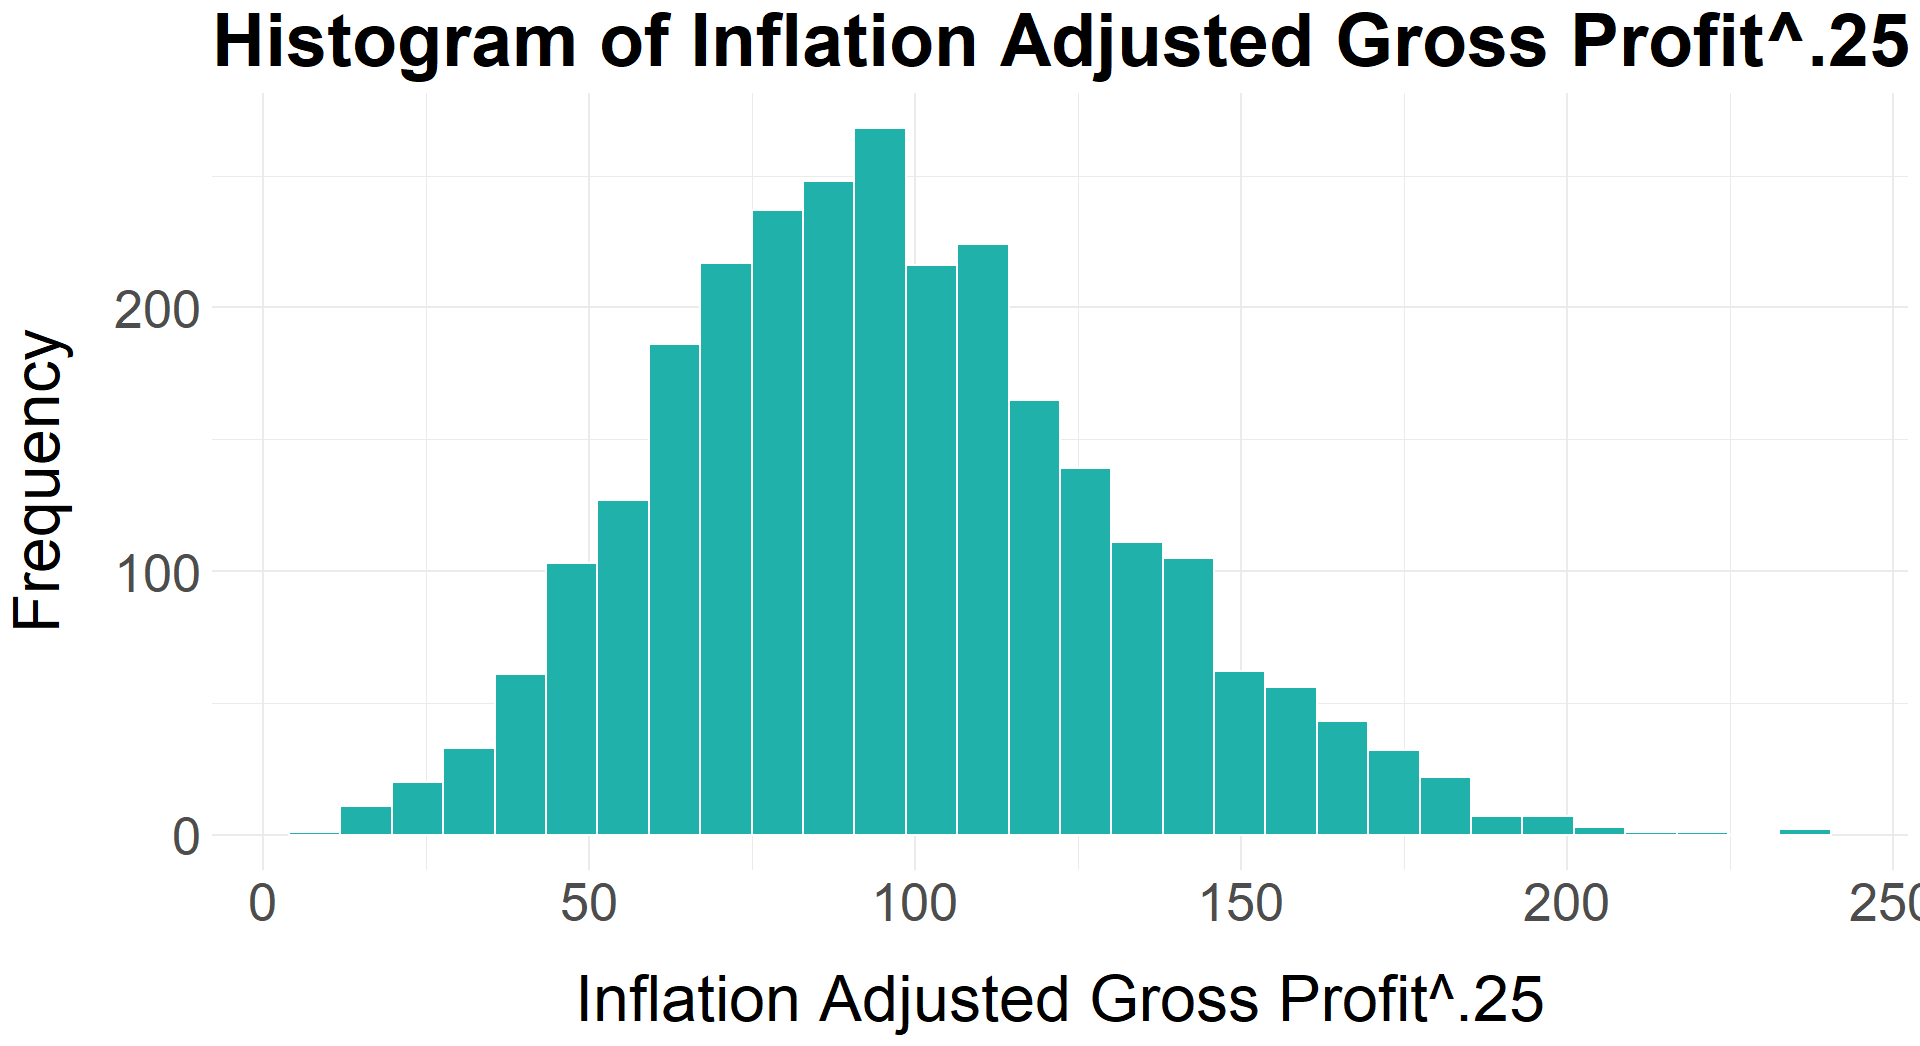
\includegraphics[width=8cm]{_assets/_eda/grossprofit_hist_t.png}
\end{center}

\subsection{Predictor Variables}

In selecting potential predictor variables, it is essential to note that we only examined variables that a movie producer can reasonably control. Our goal was not to determine which variables in our data set are the best predictors of our response variables, but to determine the most predictive variables that can be modified before a movie is made.

1 --- Runtime

The runtime variable was approximately normally distributed outside of a few outlier points. Given the size of our dataset we left the outlier points in the dataset. On average, Oscar-nominated movies had longer run times than movies that were not nominated for an Oscar. The runtime variable also showed clear signs of positive correlation with the inflation-adjusted gross profit variable.

\begin{center}
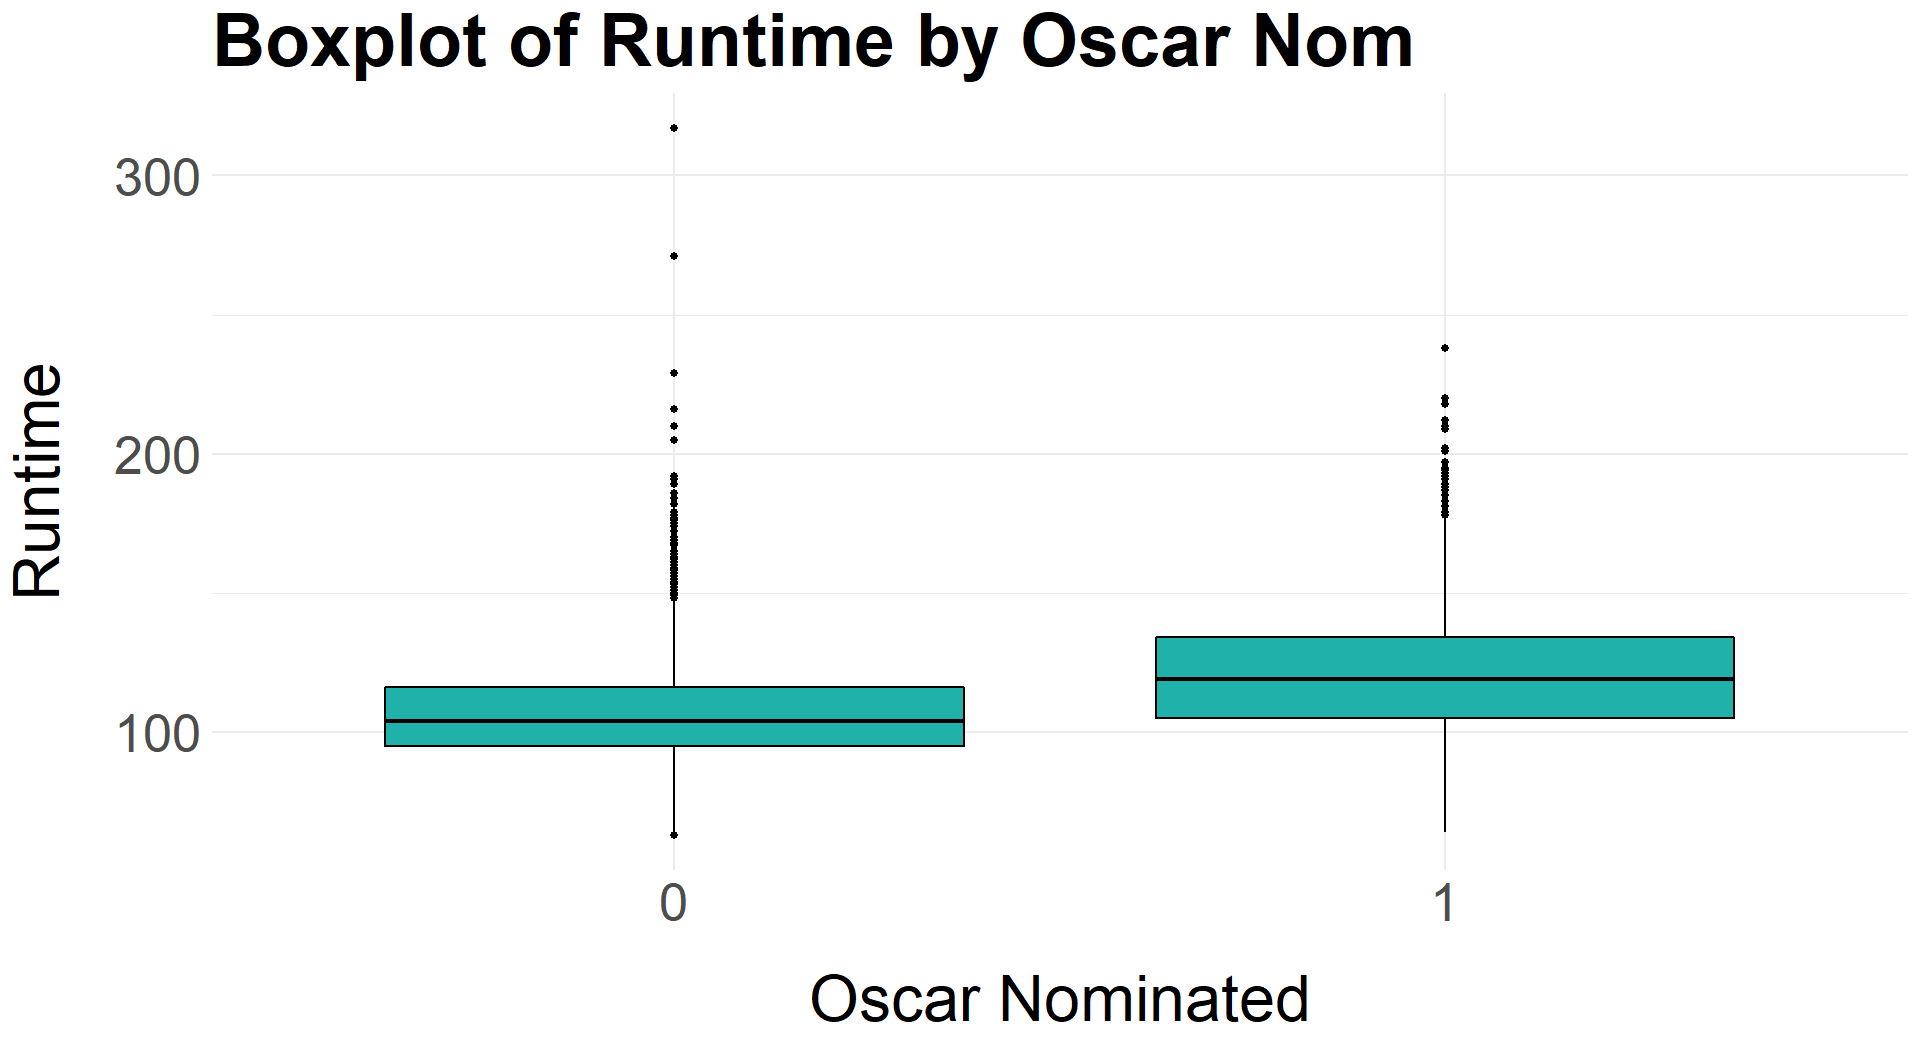
\includegraphics[width=8cm]{_assets/_eda/runtime_on.png}
\hspace{1cm}
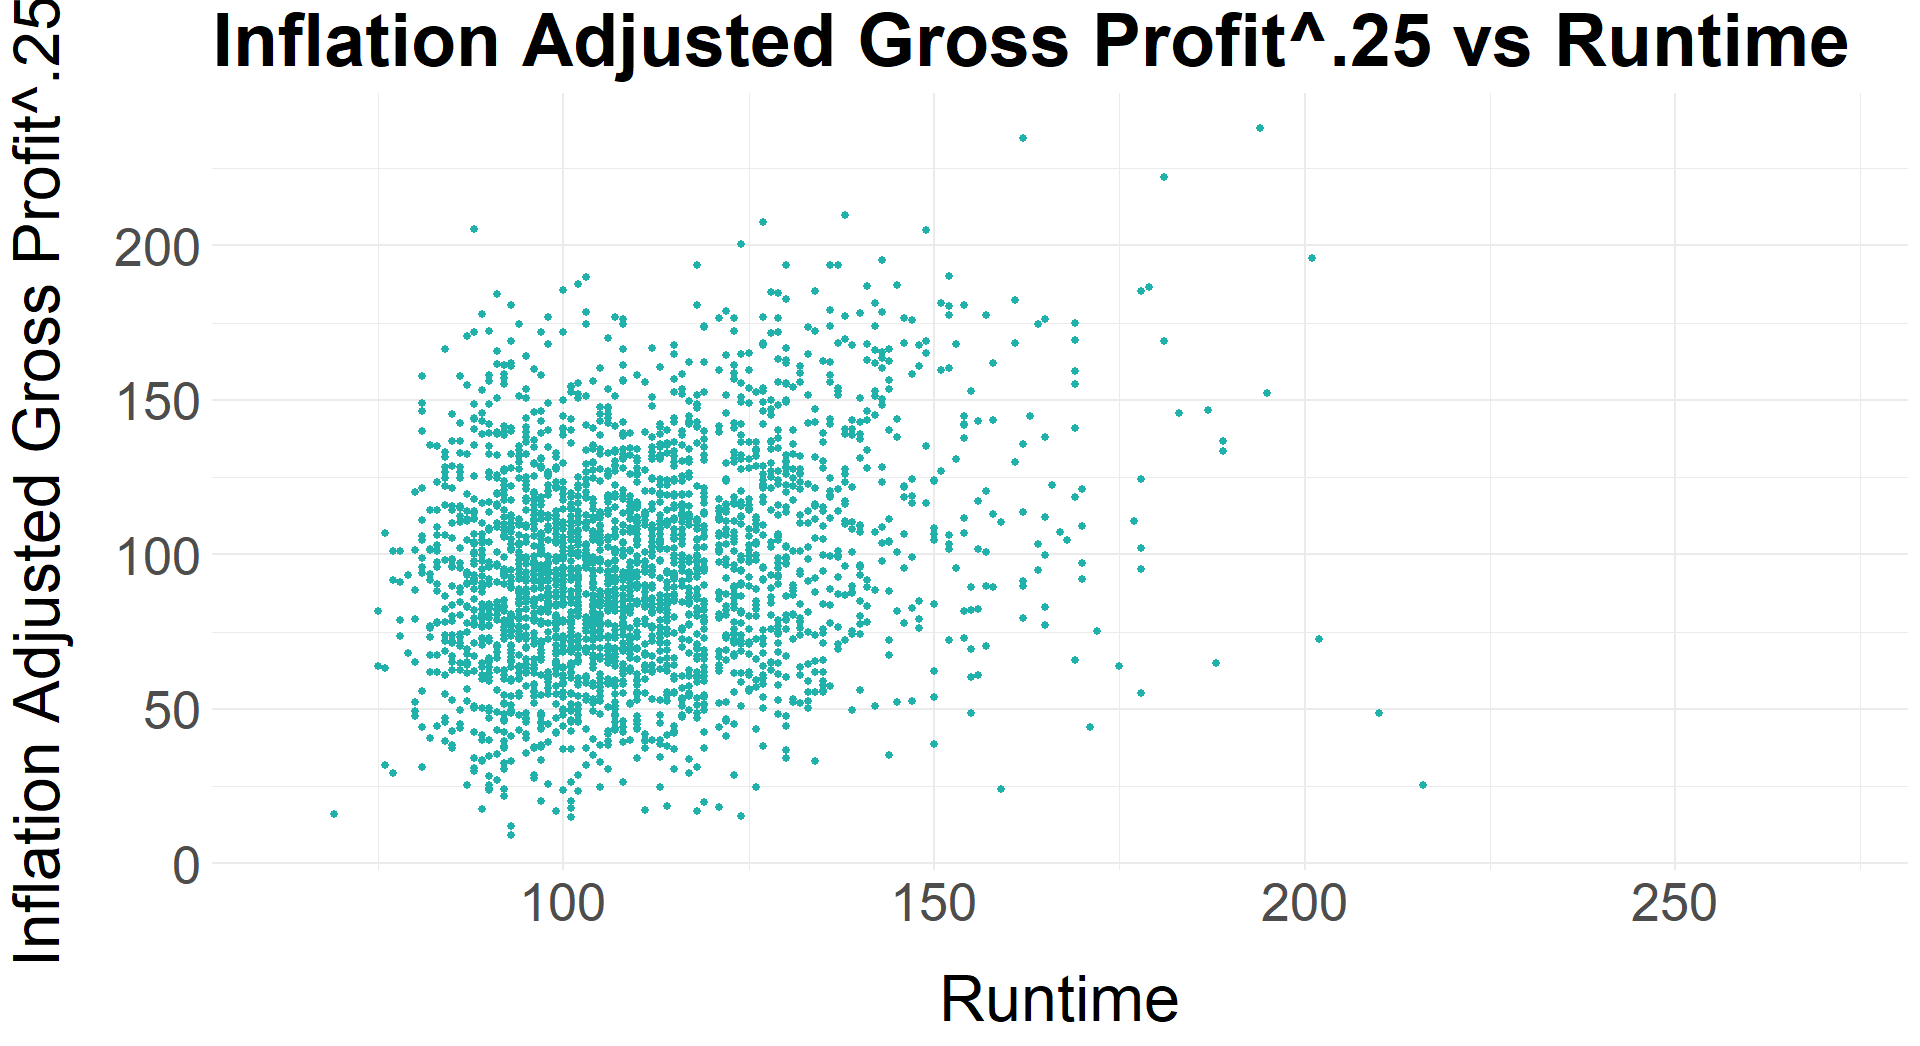
\includegraphics[width=8cm]{_assets/_eda/runtime_iagp.png}
\end{center}


2 --- Genre

We combined all genres with low frequency into a new genre called “Other” and ended up with 9 separate genre categories. The drama, other (uncommon), and adventure genres had the highest proportion of films that were nominated for an Oscar, while the horror genre had by far the lowest proportion, at just 5 percent. Interestingly enough, the drama genre actually had the lowest mean gross profit, while adventure and action had the two highest mean gross profits.

\begin{center}
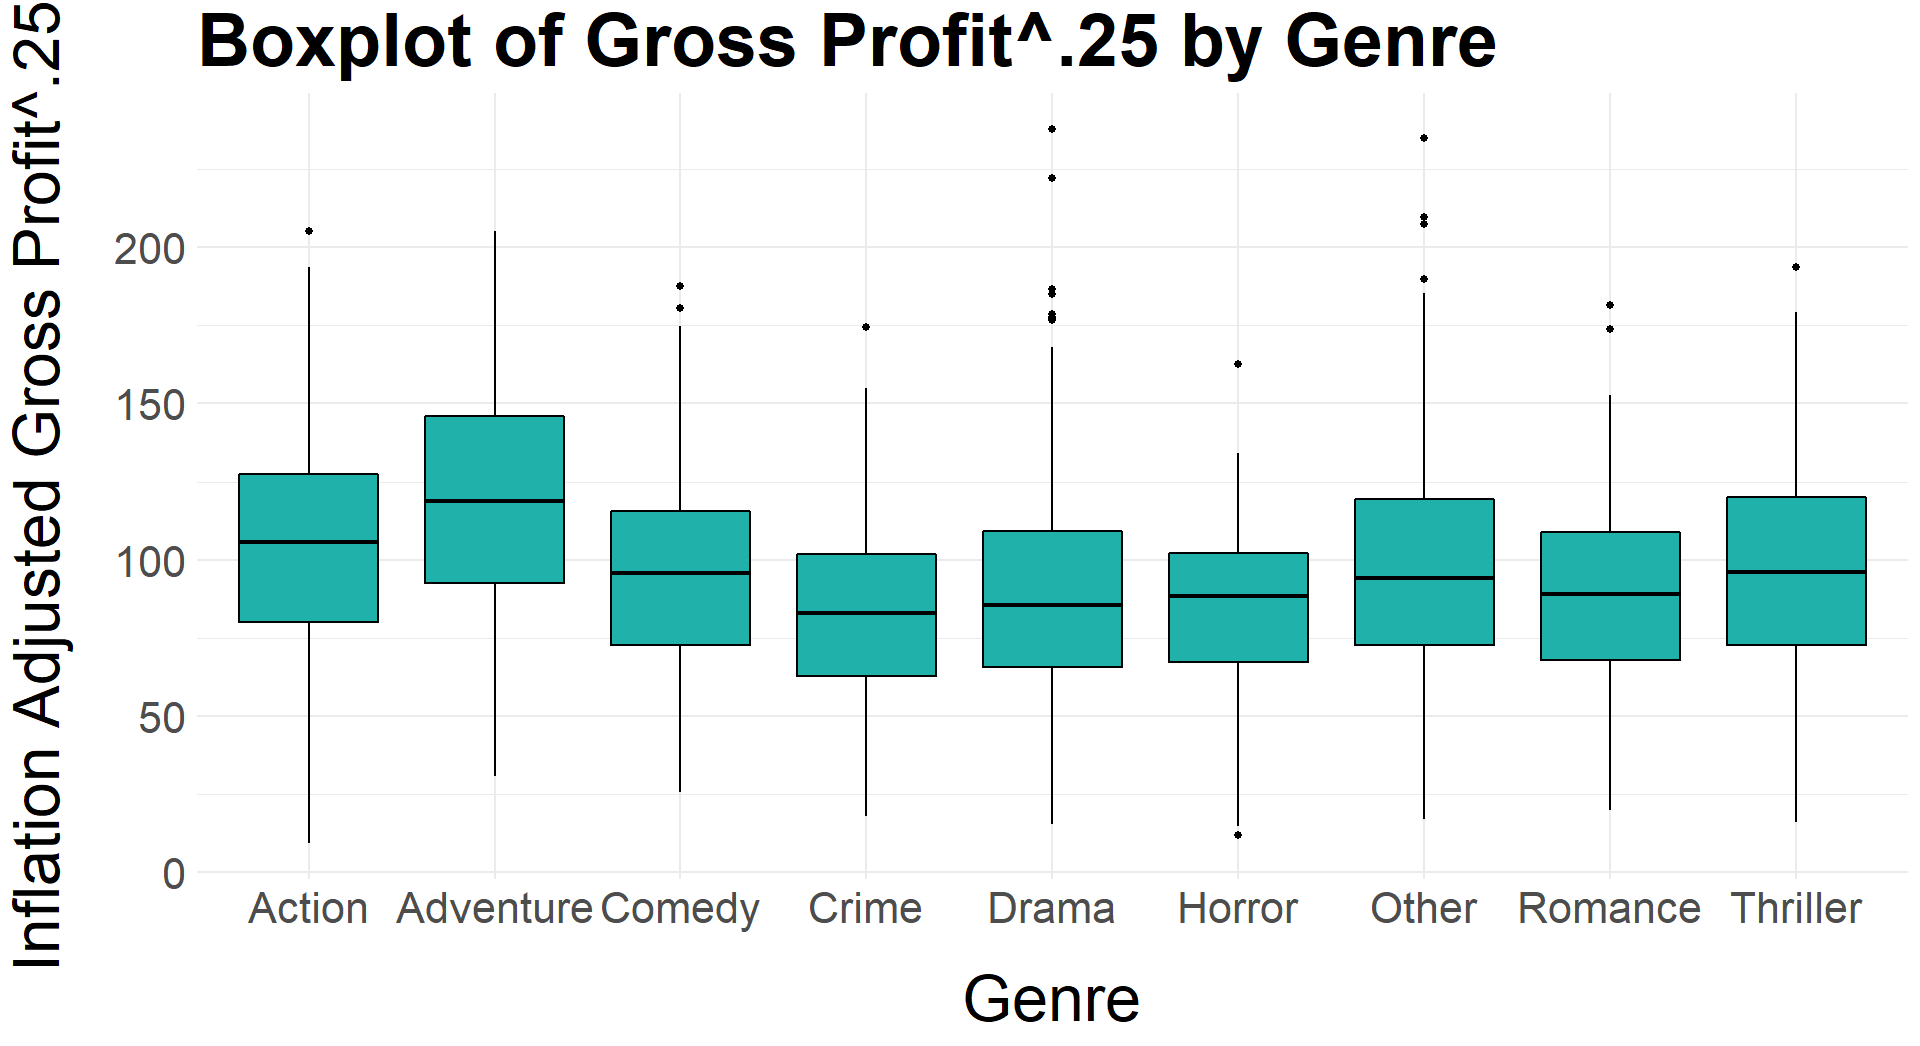
\includegraphics[width=8cm]{_assets/_eda/genre_iagp_bp.png}
\hspace{1cm}
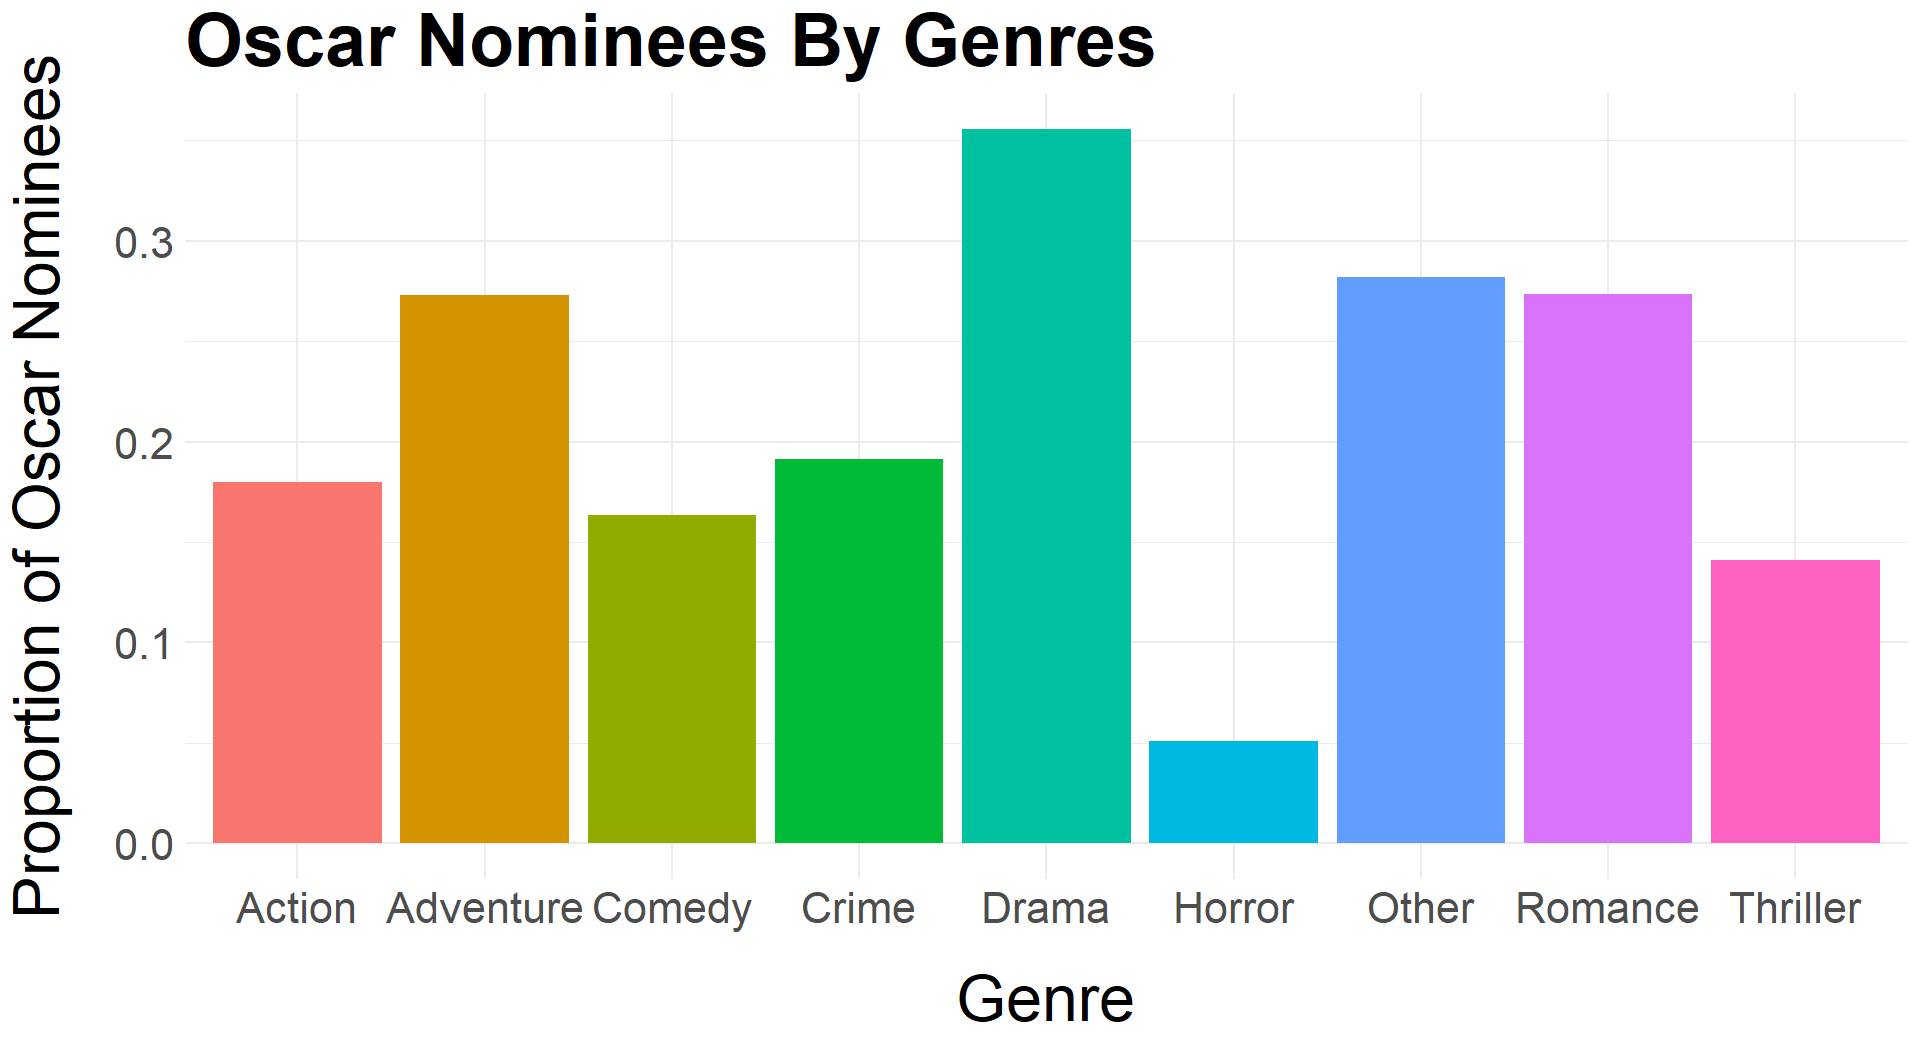
\includegraphics[width=8cm]{_assets/_eda/on_by_genre.png}
% latex table generated in R 4.1.1 by xtable 1.8-4 package
% Fri Jun  3 07:02:12 2022
\begin{table}[H]
\centering
\begin{tabular}{rrr}
  \hline
 & No Oscar Nom & Oscar Nom \\ 
  \hline
Action & 0.83 & 0.17 \\ 
  Adventure & 0.69 & 0.31 \\ 
  Comedy & 0.84 & 0.16 \\ 
  Crime & 0.82 & 0.18 \\ 
  Drama & 0.65 & 0.35 \\ 
  Horror & 0.95 & 0.05 \\ 
  Other & 0.72 & 0.28 \\ 
  Romance & 0.73 & 0.27 \\ 
  Thriller & 0.82 & 0.18 \\ 
   \hline
\end{tabular}
\caption{Genre Proportion by Oscar Nom} 
\label{tab:gnon}
\end{table}


\end{center}

3 --- Rating

Similar to genre, we reduced the levels of the parental guideline rating variable to the following four: PG, PG-13, R, Other. Surprisingly, movies rated PG had the highest proportion of Oscar nominations at 34 percent, with the other three categories all having nearly identical proportions of Oscar nominations at about 22 percent. Movies rated PG also had the highest mean gross profit, followed by PG-13 rated movies. 

\begin{center}
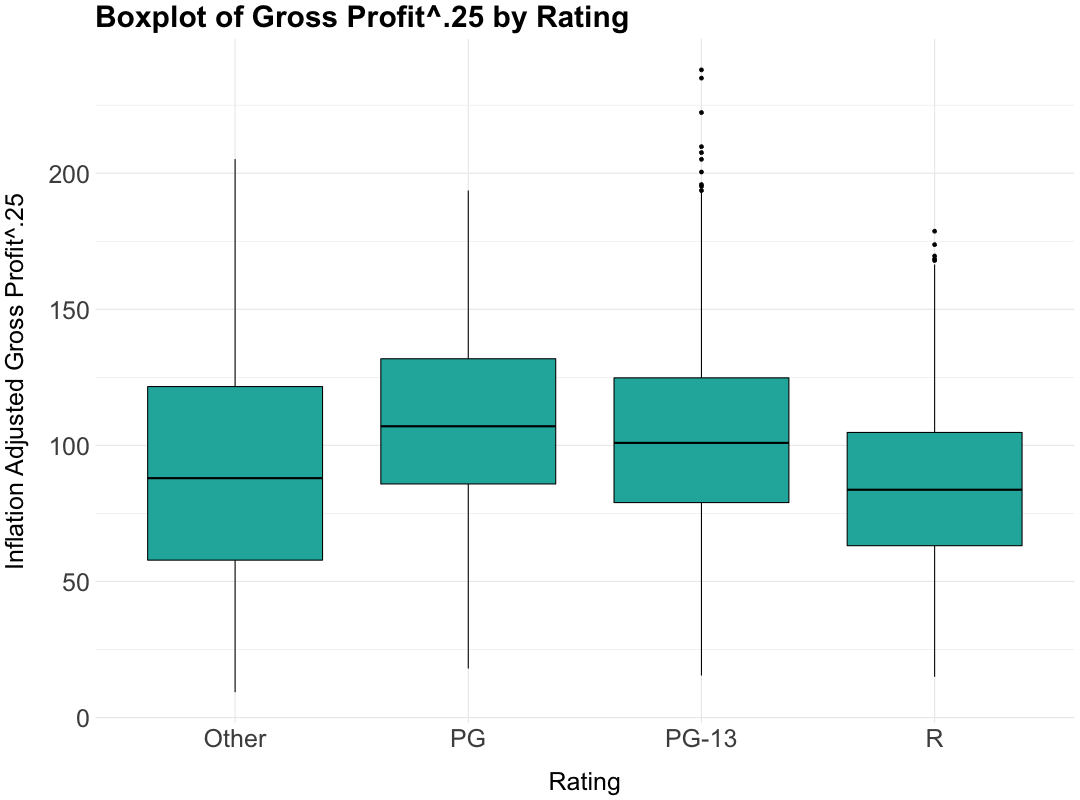
\includegraphics[width=8cm]{_assets/_eda/rating_iagp_bp.png}
% latex table generated in R 4.1.1 by xtable 1.8-4 package
% Fri Jun  3 06:58:11 2022
\begin{table}[H]
\centering
\begin{tabular}{rrr}
  \hline
 & No Oscar Nom & Oscar Nom \\ 
  \hline
Other & 0.77 & 0.23 \\ 
  PG & 0.66 & 0.34 \\ 
  PG-13 & 0.78 & 0.22 \\ 
  R & 0.78 & 0.22 \\ 
   \hline
\end{tabular}
\caption{Rating Proportion by Oscar Nom} 
\label{tab:ron}
\end{table}


\end{center}

4 --- Language

The language variable had over 100 unique values. We reduced the categories to “English” and “Multilingual / Foreign” where “English” means the movie can be watched in English only and “Multilingual / Foreign” means the movie can be watched in several languages or in a non-English language only.

% latex table generated in R 4.2.0 by xtable 1.8-4 package
% Mon Jun  6 19:10:52 2022
\begin{table}[H]
\centering
\begin{tabular}{rr}
  \hline
No Oscar Nom & Oscar Nom \\ 
  \hline
0.41 & 0.11 \\ 
  0.35 & 0.13 \\ 
   \hline
\end{tabular}
\caption{Language Proportion by Oscar Nom} 
\end{table}



5 --- Star Power

The star power variable was slightly skewed, but for the sake of interpretation, it is better to leave the variable as-is. Films nominated for Oscars generally had higher star power although the differences in means were not drastic. Plotting star power vs inflation-adjusted gross profit showed some signs of positive correlation, though the correlation was not nearly as strong as the runtime correlation.

\begin{center}
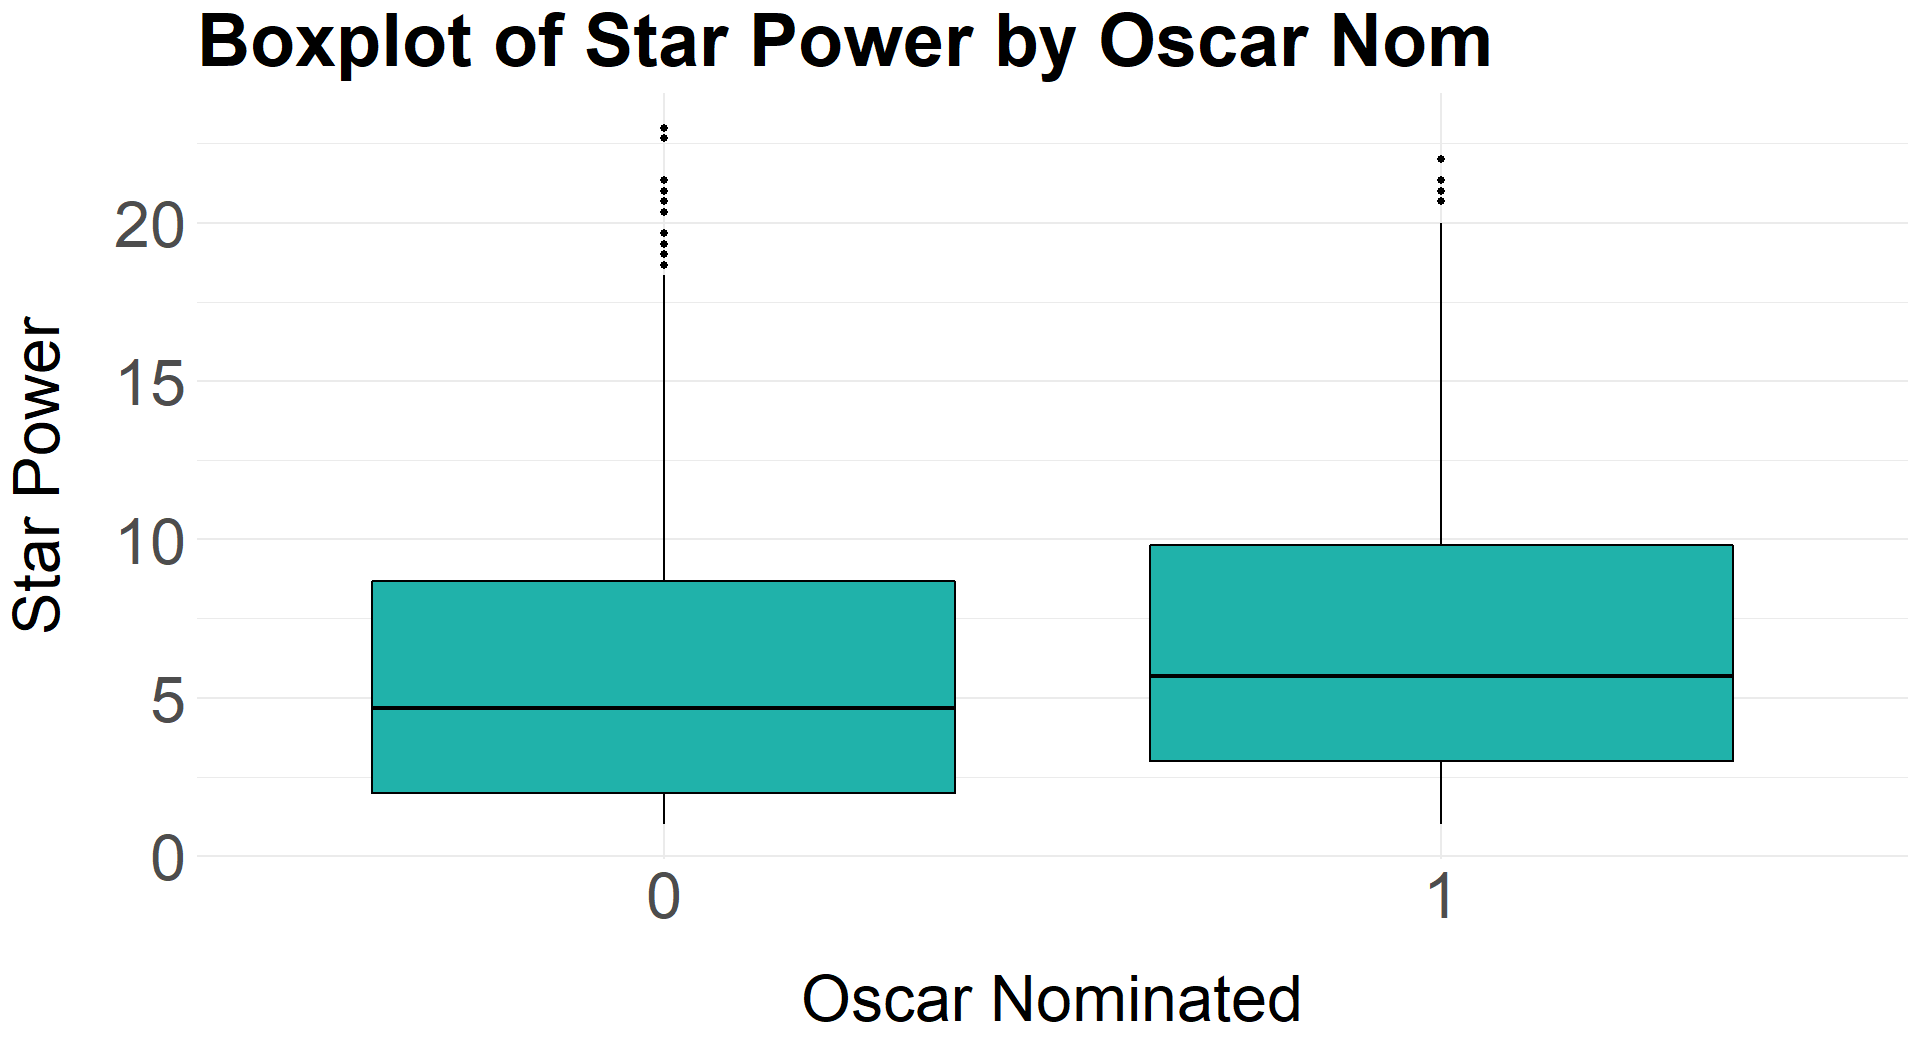
\includegraphics[width=8cm]{_assets/_eda/star_power_on.png}
\hspace{1cm}
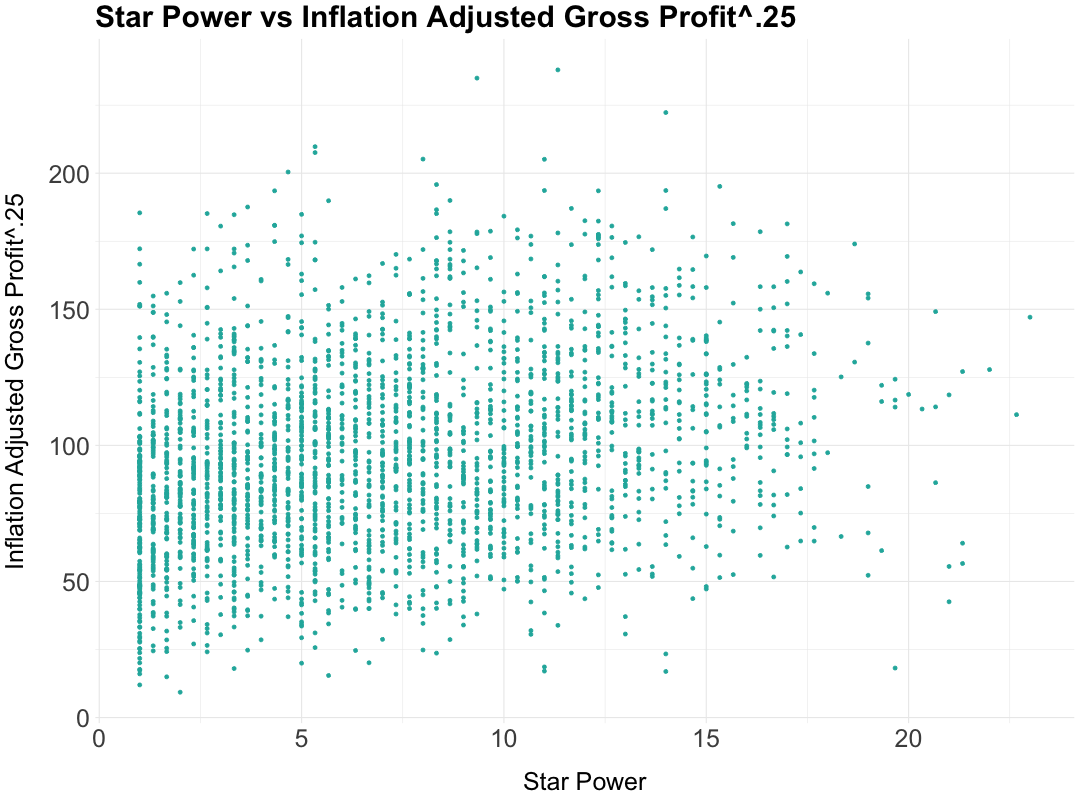
\includegraphics[width=8cm]{_assets/_eda/star_power_iagp.png}
\end{center}

6 --- Writer Popularity

The writer popularity variable was also slightly skewed, but for the sake of model interpretability, we chose to leave the variable as-is. While the mean writer popularity of Oscar-nominated films was nearly identical to the mean writer popularity of films not nominated, the variable did show signs of higher correlation with inflation-adjusted gross profit than the star power variable had. 

\begin{center}
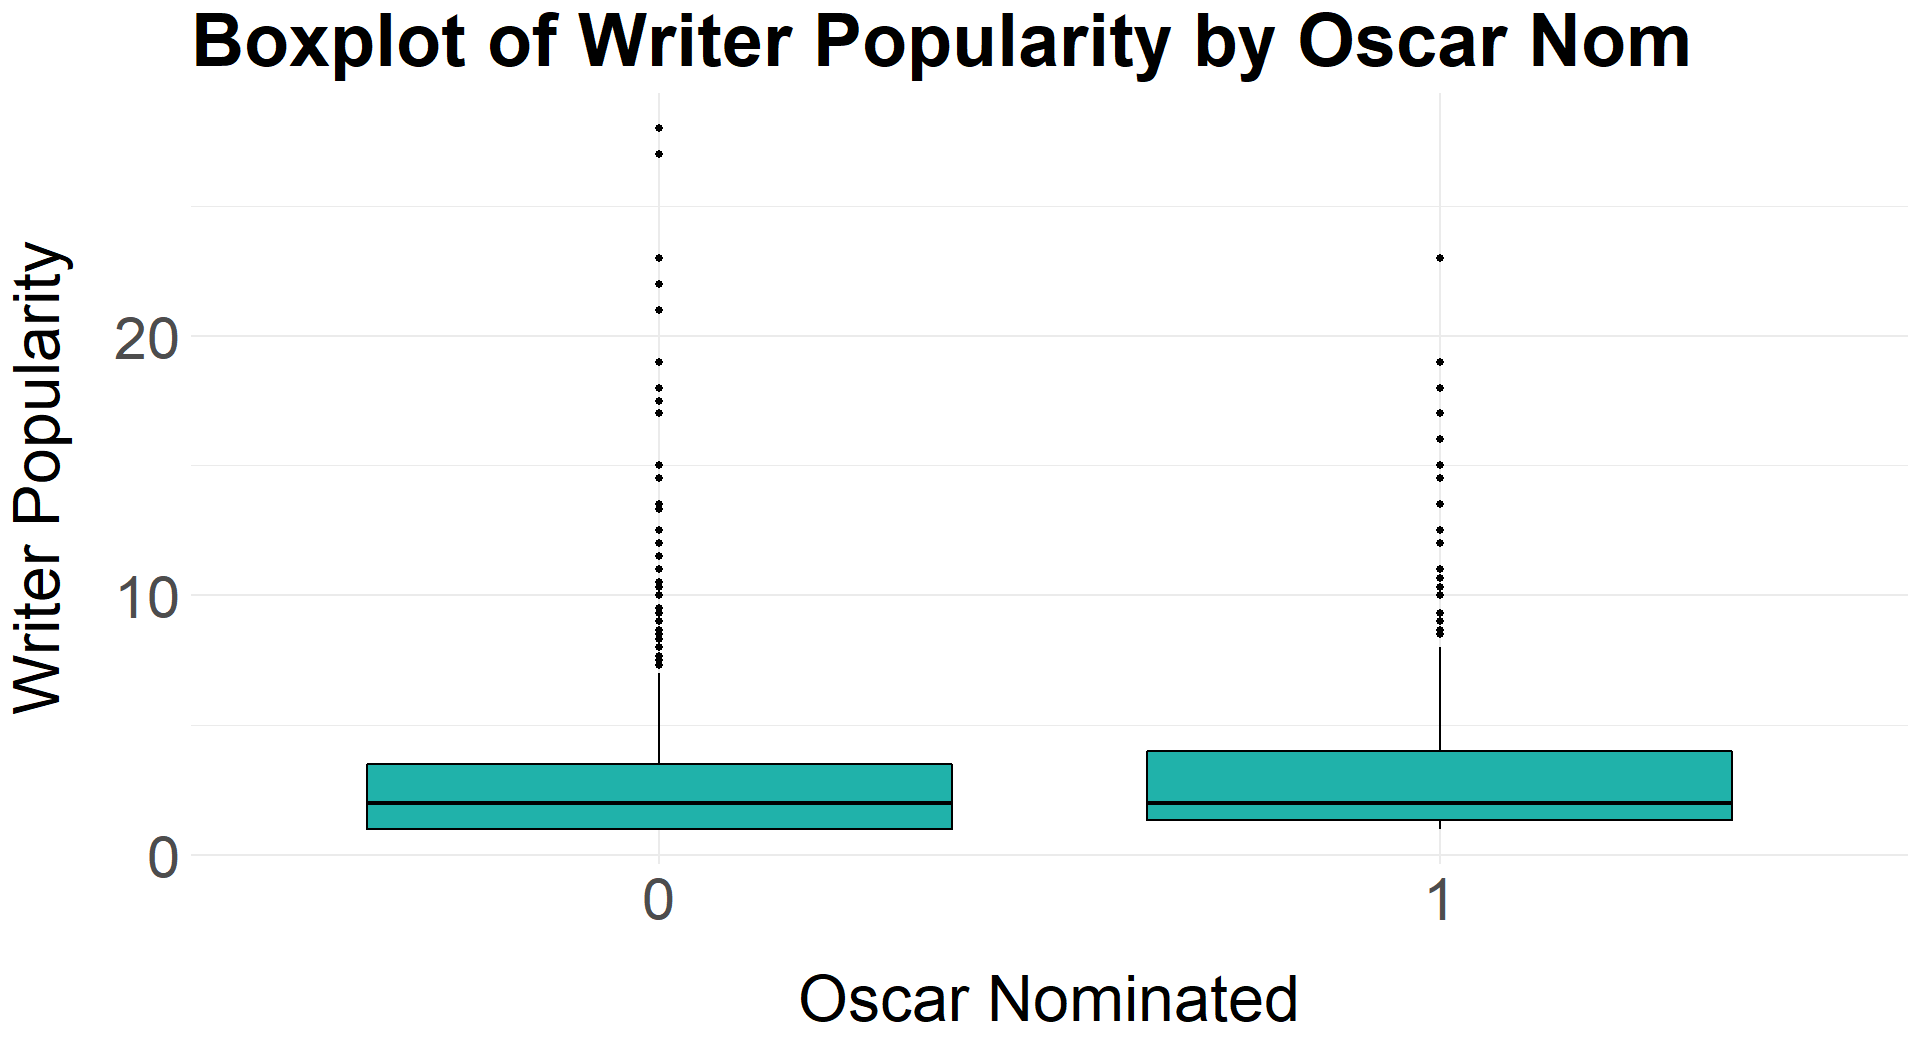
\includegraphics[width=8cm]{_assets/_eda/writer_pop_on.png}
\hspace{1cm}
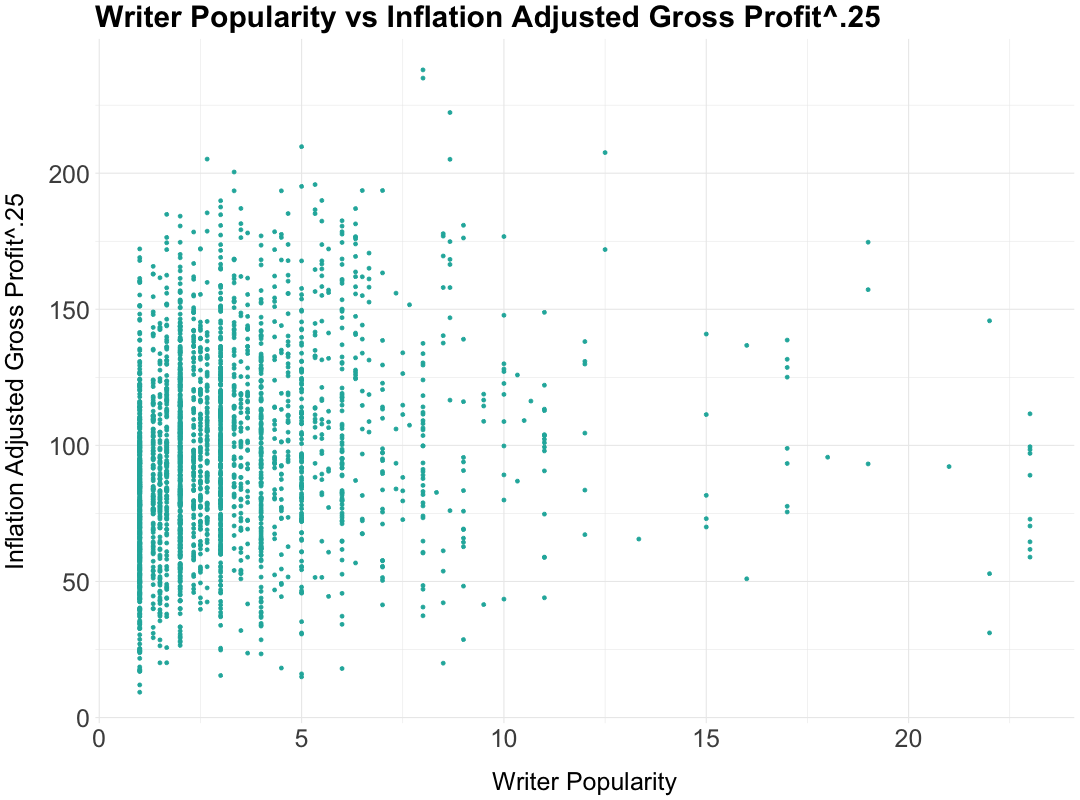
\includegraphics[width=8cm]{_assets/_eda/writer_pop_iagp.png}
\end{center}

7 --- Director Popularity

The director popularity variable was heavily right-skewed, which is unsurprising given the fact that we only used a single director’s popularity, versus average popularity of multiple stars in the star power variable. Despite transformation attempts, the variable distribution remained skewed. Therefore, we decided to transform it into a factor variable with 4 levels based on approximately equal frequencies. 

Directors that appeared the least amount of times in the data set were only nominated for an Oscar 12 percent of the time compared to directors that appeared the most amount of times in the data set who were nominated for an Oscar 35 percent of the time. Director popularity was also strongly correlated with inflation-adjusted gross profit, with each level showing an incremental increase in mean gross profit. 

\begin{center}
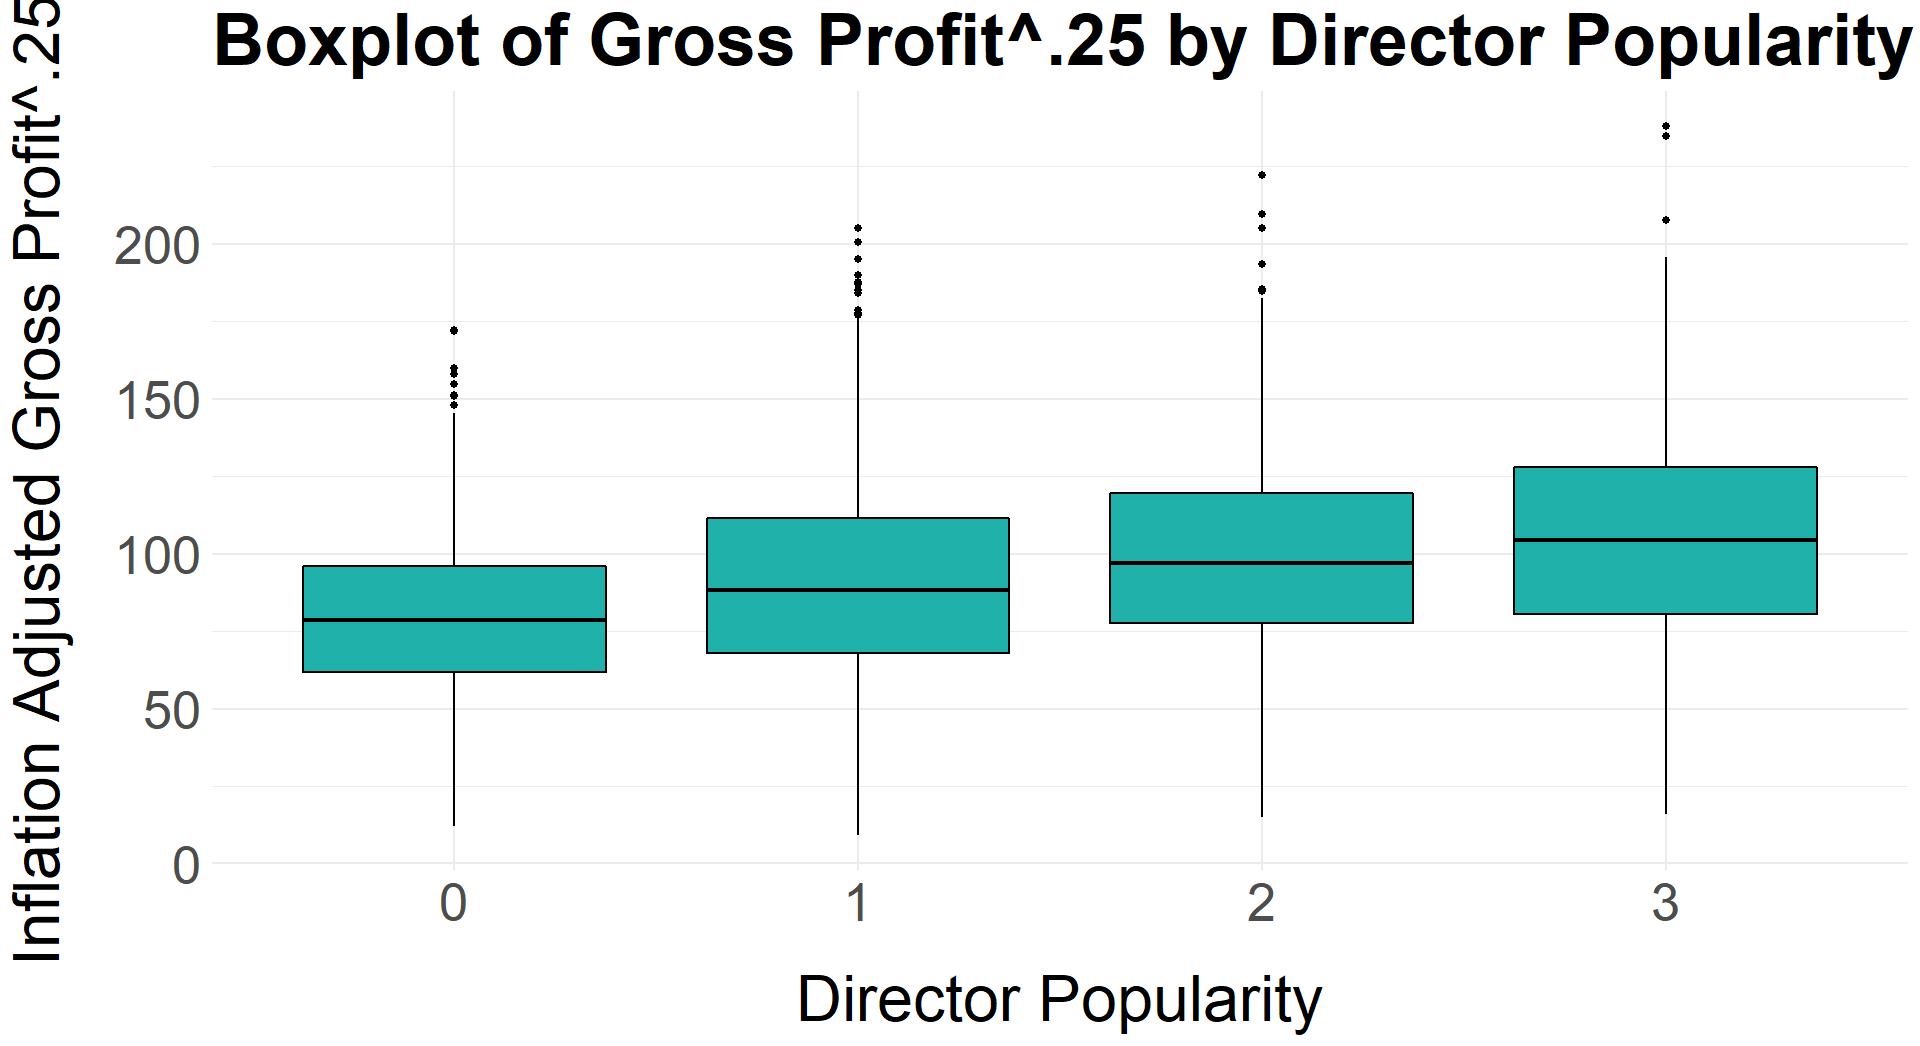
\includegraphics[width=8cm]{_assets/_eda/dir_pop_iagp_bp.png}
% latex table generated in R 4.1.1 by xtable 1.8-4 package
% Fri Jun  3 06:59:15 2022
\begin{table}[H]
\centering
\begin{tabular}{rrr}
  \hline
 & No Oscar Nom & Oscar Nom \\ 
  \hline
0 & 0.88 & 0.12 \\ 
  1 & 0.78 & 0.22 \\ 
  2 & 0.76 & 0.24 \\ 
  3 & 0.65 & 0.35 \\ 
   \hline
\end{tabular}
\caption{Director Popularity Proportion by Oscar Nom} 
\label{tab:don}
\end{table}


\end{center}

8 --- Production Company Size

Similar to the director variable, the company size variable was heavily skewed. Again, we decided to turn the numerical variable into a factor variable with 4 levels based on even quantiles. Larger companies generally had slightly higher proportions of Oscar-nominated films although the second-highest category actually had the largest proportion of nominations at 29 percent. Company size was more strongly correlated with inflation-adjusted gross profit, with clear steps up in mean gross profit between each level. 

\begin{center}
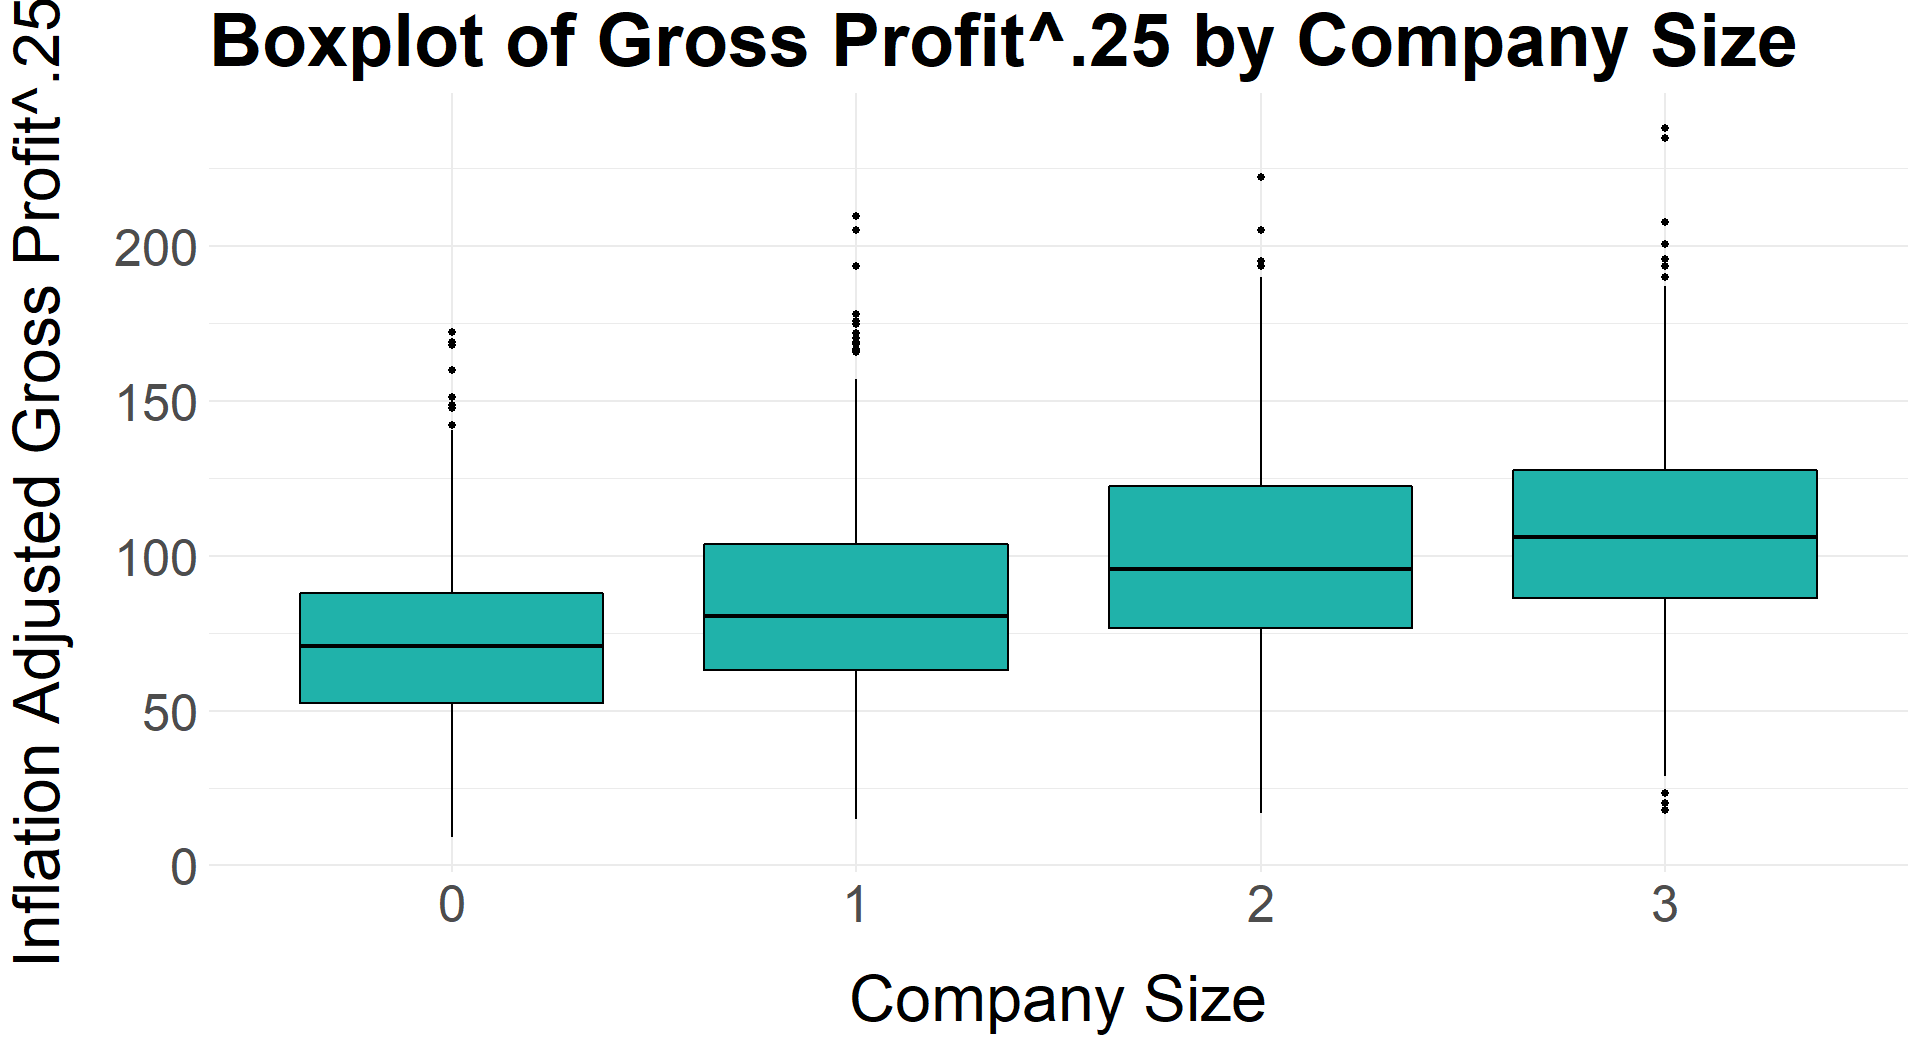
\includegraphics[width=8cm]{_assets/_eda/co_size_iagp_bp.png}
% latex table generated in R 4.1.1 by xtable 1.8-4 package
% Fri Jun  3 06:59:24 2022
\begin{table}[H]
\centering
\begin{tabular}{rrr}
  \hline
 & No Oscar Nom & Oscar Nom \\ 
  \hline
0 & 0.79 & 0.21 \\ 
  1 & 0.80 & 0.20 \\ 
  2 & 0.71 & 0.29 \\ 
  3 & 0.74 & 0.26 \\ 
   \hline
\end{tabular}
\caption{Company Size Proportion by Oscar Nom} 
\label{tab:con}
\end{table}


\end{center}

9 --- Release Period

Starting with release months, we wanted to reduce the levels of the categorical variable from 12 down to 4. We used the holiday season (November-January) as our starting point and grouped every 3 months sequentially. The period right before the Oscars (November-January) had the highest proportion of Oscar nominations at 36 percent, compared to the period right after the Oscars (February-April) which only had 17 percent of films nominated. In terms of gross profit, the beginning of summer (May-July) generally produced the largest amount of profit, with the holiday season (November-January) producing the second-largest profit. 

\begin{center}
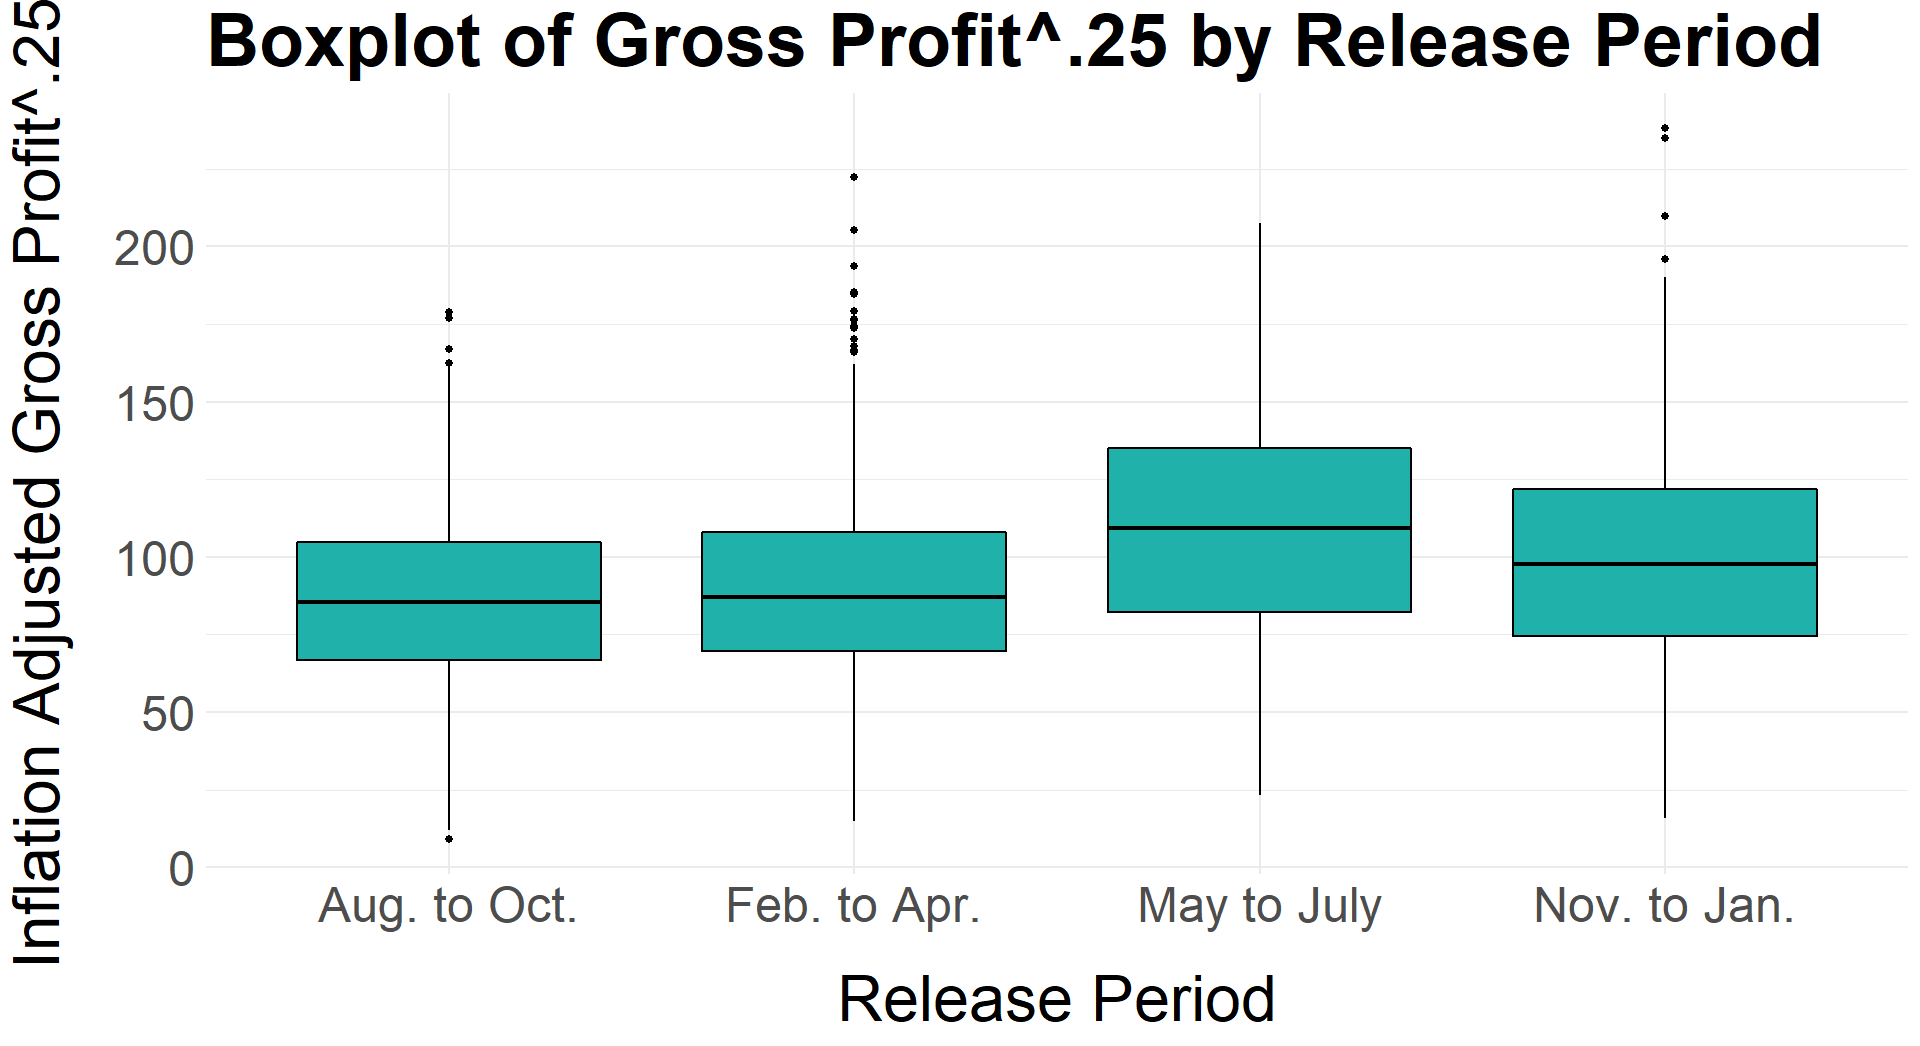
\includegraphics[width=8cm]{_assets/_eda/releaseperiod_iagp_bp.png}
\hspace{1cm}
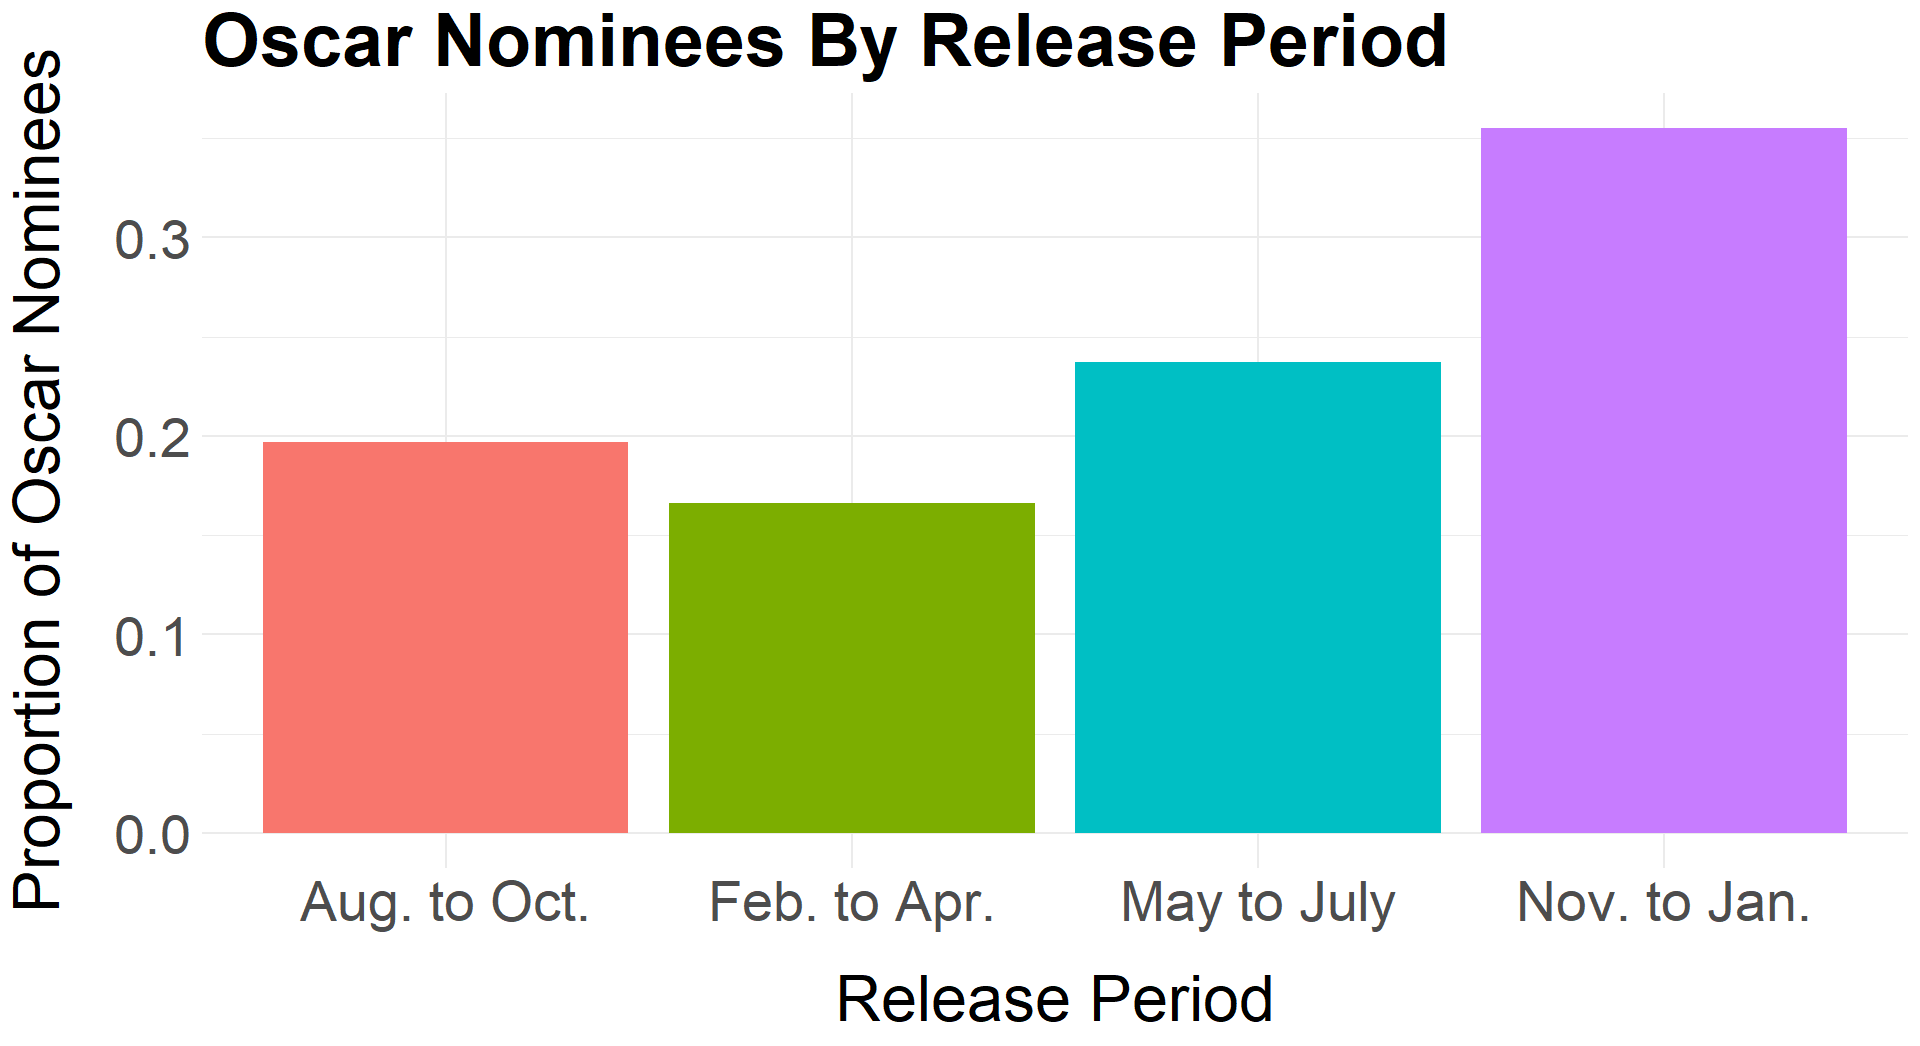
\includegraphics[width=8cm]{_assets/_eda/on_by_release_period.png}
% latex table generated in R 4.1.1 by xtable 1.8-4 package
% Fri Jun  3 06:59:36 2022
\begin{table}[H]
\centering
\begin{tabular}{rrr}
  \hline
 & No Oscar Nom & Oscar Nom \\ 
  \hline
aug\_to\_oct & 0.80 & 0.20 \\ 
  feb\_to\_apr & 0.83 & 0.17 \\ 
  may\_to\_jul & 0.76 & 0.24 \\ 
  nov\_to\_jan & 0.64 & 0.36 \\ 
   \hline
\end{tabular}
\caption{Release Period Proportion by Oscar Nom} 
\label{tab:rpon}
\end{table}


\end{center}
	
10 --- Inflation-Adjusted Budget

The inflation-adjusted budget variable was also skewed but again for interpretability, we decided against transforming the variable. Oscar-nominated films generally had higher budgets although the difference in means did not appear to be very significant. However, the inflation-adjusted budget certainly demonstrated signs of positive correlation with the transformed gross profit.

\begin{center}
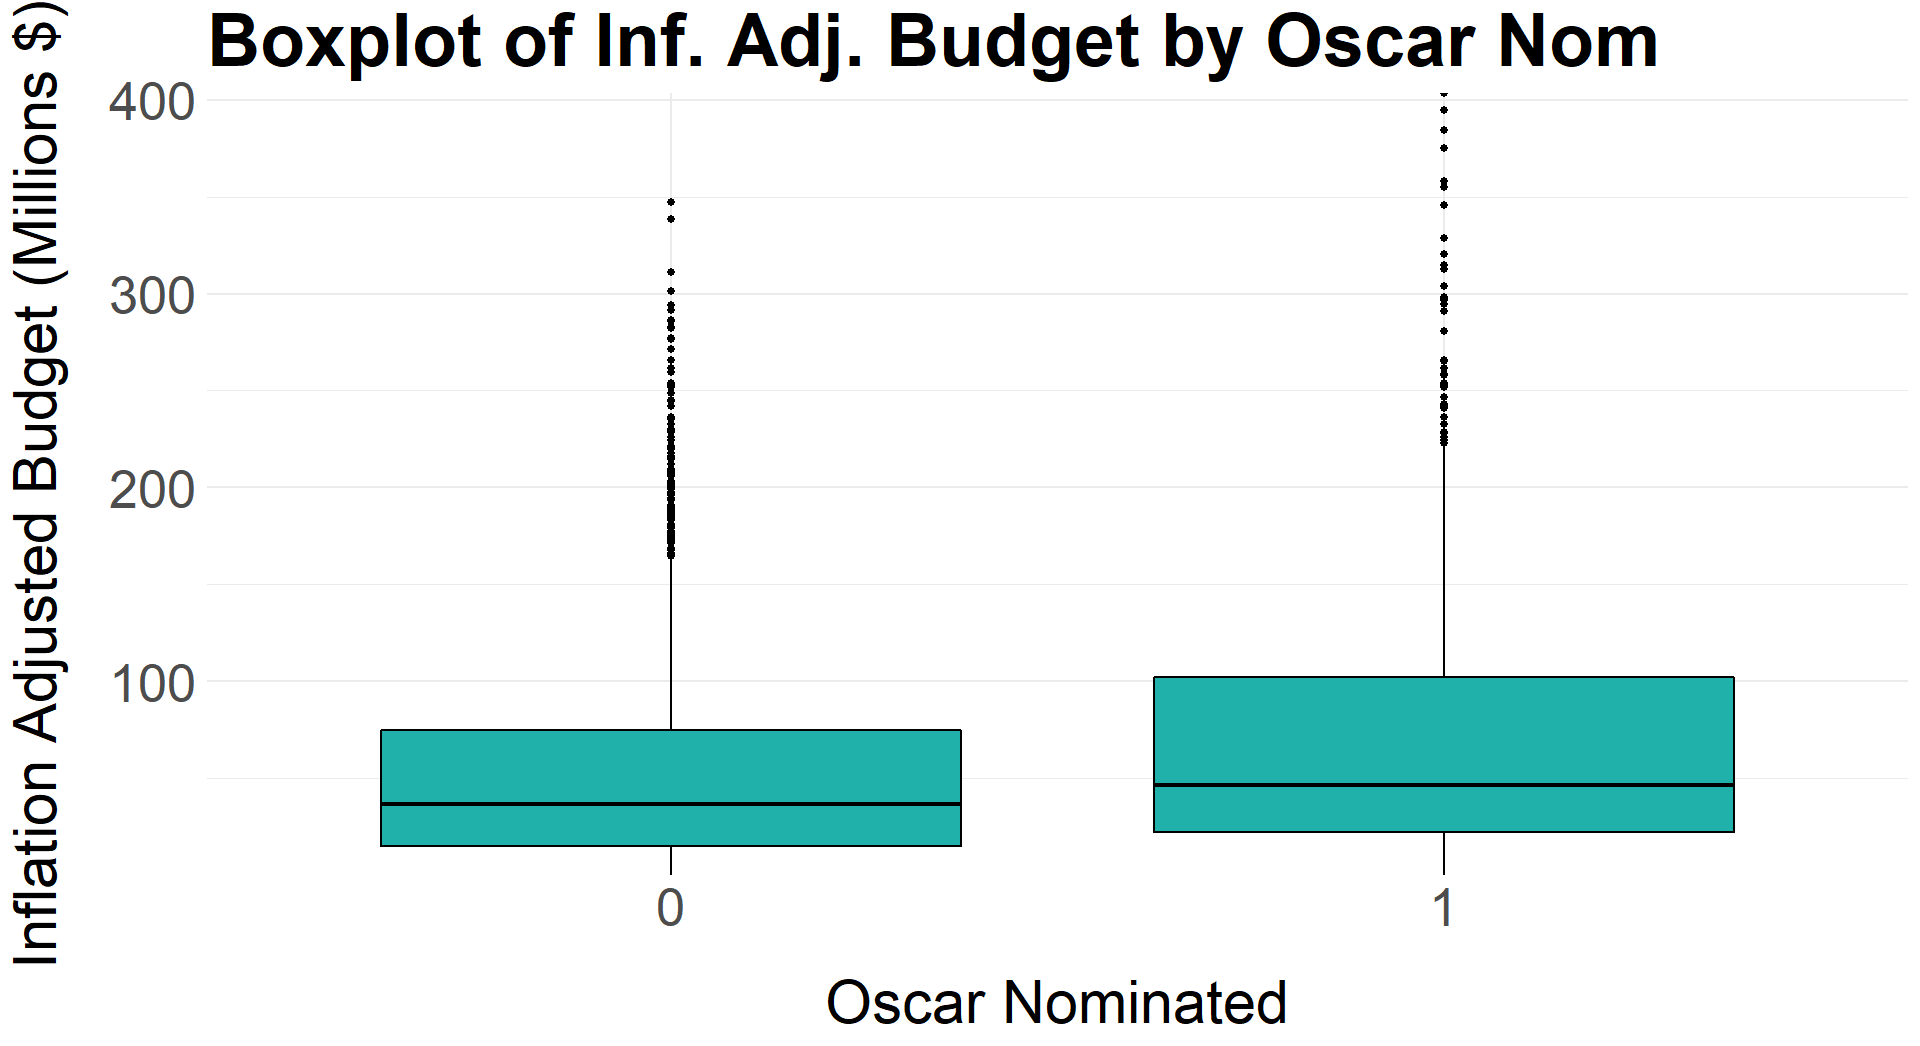
\includegraphics[width=8cm]{_assets/_eda/budget_on.png}
\hspace{1cm}
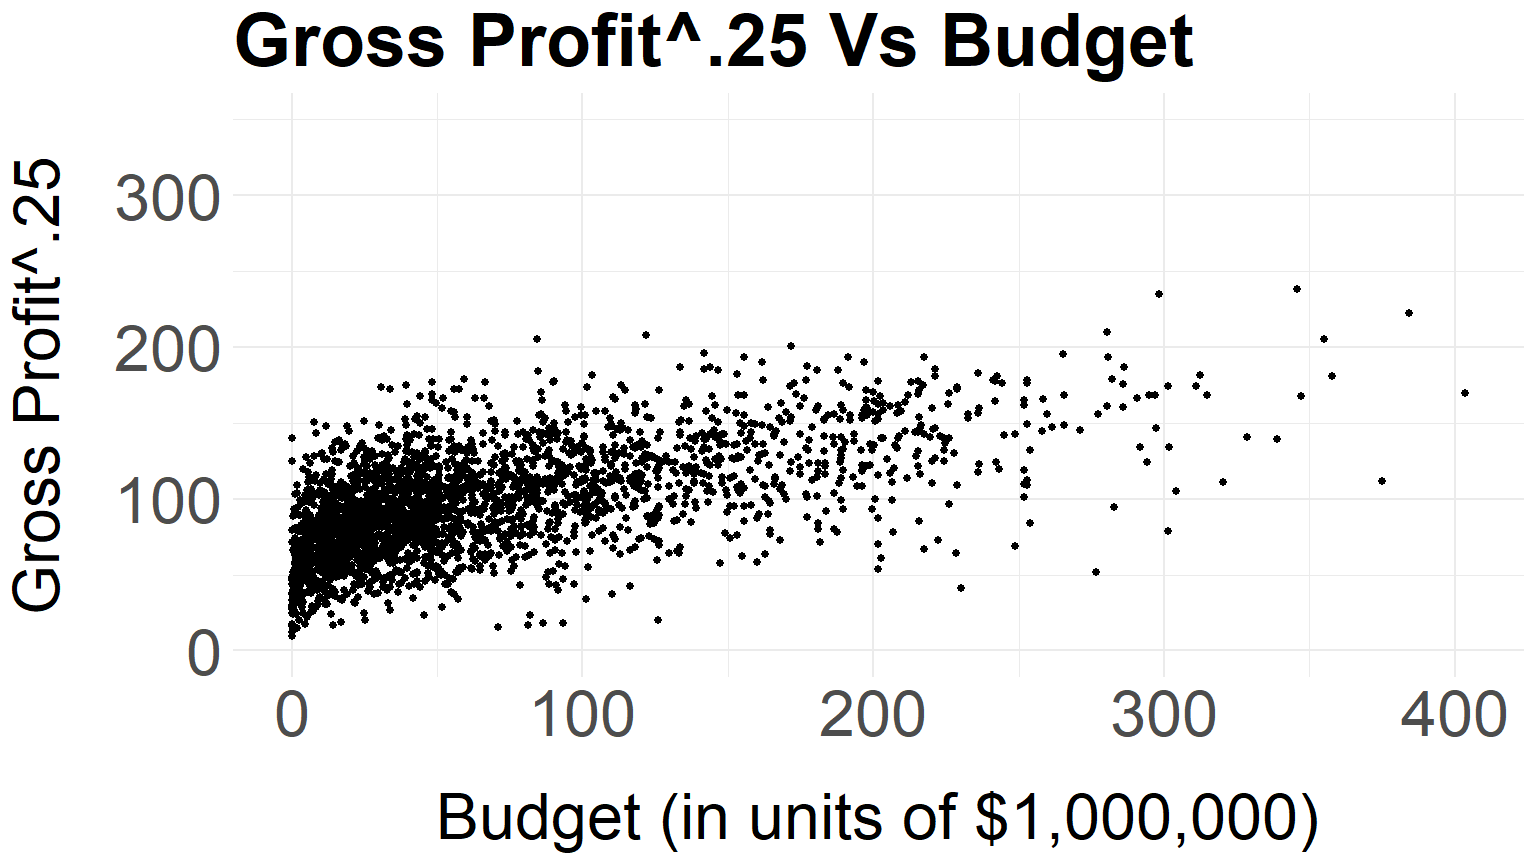
\includegraphics[width=8cm]{_assets/_eda/budget_v_profit25_corr_plot.png}
\end{center}

\section{Methodology}

\subsection{Model and Maximize Box Office Profits}

In this section, we will discuss how we developed our models. Not only can these models be used to estimate our expected box office profit based on a few production choices, but many features of these models may be used to provide insights into which variables are more influential in predicting box office profit. This information can then be leveraged by producers to maximize their expected returns.

The model development process for box office profits was quite iterative, with each iteration involving important additions to improve interpretability, increase accuracy, and reduce error. Since our dataset contains a variety of categorical and numeric variables, we initially decided to use a highly interpretable regression tree model to predict box office profits. The regression tree used variables from the dataset to partition the data into smaller chunks. At each partition, the tree used one explanatory variable to form a binary split on that variable and, in this case, it chose the split that minimized the Residual Sum of Squares (RSS) for our box office profit data. To decrease the chance of overfitting, we pruned the tree using a complexity parameter that prevented any unnecessary splits. 

This first iteration of our model had excellent interpretability, however, its predictive performance could be improved upon. Although a linear regression model may seem like a great alternative, one concern we had is that the encoded categorical variables (such as the encodings for genre or rating) could produce severe multicollinearity, which would lower our model’s accuracy. Therefore, we continued to use a tree based model, but to increase performance, we leveraged bootstrap resampling techniques. In order to prevent generating overly correlated regression trees when resampling, we restricted each regression tree to only use a random selection of the variables in our dataset so that they do not end up partitioning the data in exactly the same manner. This way, we can use the aggregate of highly diverse trees for our resulting model. This method of resampling is known as a \textit{Random Forest} model. Thus, to increase predictive performance we decided to fit our data with a random forest instead of with the single pruned regression tree. 

In order to optimize the random forest for our dataset, we tuned the following two hyper-parameters:

\begin{enumerate}
\item The total number of trees to generate (bootstrap resamples) 
\item The number of randomly selected variables to sample from our variable set when generating each regression tree
\end{enumerate}

While one appeal to random forests is their robustness to overfitting, a random forest can overfit its training data if too many variables are randomly selected. For this reason, we used 10-fold cross validation and collected the Root-Mean-Square Error (RMSE) and R-Squared metrics from each fold while tuning both hyper-parameters. We plotted the average RMSE and the R-Squared for each combination of parameters, and chose the pair of parameters that provided a low average RMSE while maintaining a high average R-Squared (averaged over the folds). 

At this stage, we optimized our random forest model as much as possible. However, we do not only need powerful predictive capabilities from our model. We would also like to be able to interpret our model. Knowing which features are most predictive of box office profit tells us which features a producer should prioritize, or value over others. Furthermore, we calculated variable importance from our trained random forest using the \textit{Permutation Importance} method. The Permutation Importance method records a baseline R-Squared score with our trained random forest, permutes the observation values of a single predictor variable, recomputes the R-Squared with the trained random forest, and then compares the new R-Squared score to the baseline R-Squared score. Iteratively performing this process for each predictor variable in the training data provides a measure of feature importance by looking at how much the R-Squared decreases when a feature is effectively unavailable. Variables with higher permutation importance demonstrate greater ability to predict box office profit, so we plotted each variable’s “importance” value in descending order to emphasize each feature’s relative value. 

We concluded our box office profit analysis by comparing our newly established random forest model to a standard linear model using only the numeric variables in our dataset (to prevent any negative effects from multicollinearity). We compared the RMSE and R-Squared metrics between the two models to determine the relative predictive power for each model. Recall that coefficients in a linear regression model are commonly interpreted as a form of feature importance, assuming all predictor variables are on the same scale. That is, in general, the larger the coefficient in a linear model, the greater the “importance” of the corresponding predictor variable. Therefore, we compare the coefficients of the linear model to the permutation importance values reported from our random forest. In this case, we would expect that the coefficients in the linear model support our permutation importance values from our random forest (i.e. variables corresponding to higher coefficients in the linear model also correspond to higher permutation importance values in the random forest).  

\subsection{Model and Maximize Chances of an Academy Award Nomination}

Although a large box office return may be considered a financial success, if our goal is to receive critical acclaim, financial metrics may not be as relevant to a producer as, say, the chances of receiving an Academy Award. In this section, we review the statistical methods we used to estimate the probability of receiving an Academy Award (Oscar) nomination. 

The primary difference between the Oscar nomination model and the box office profit model from the last section is that Oscar nominations is a \textit{binary response variable} and box office profit is a \textit{continuous response variable}. That is, our model should predict whether or not a given movie is nominated for an Oscar based on specific attributes of the movie. This is known as a \textit{binary classification} model. A binary classification model predicts the binary class label, while regression models predict the continuous quantity.

Since we are using a similar set of variables from the dataset we used in the previous section, we began modeling Oscar nominations using a random forest. In this case, our random forest model will output probabilities associated with being nominated for an Oscar or not. Similar to the random forest model developed for the box office predictions, this model leverages bootstrap resampling techniques to generate many trees. The trees, however, are now called \textit{classification trees}, since each tree is attempting to classify movies as Oscar nominees or not. The primary difference between classification trees and regression trees is that instead of partitioning the data to minimize the RSS, the data is partitioned by minimizing the Gini impurity index. Generally speaking, the Gini index is a measure of estimated probability of misclassification, and is determined by subtracting the sum of squared proportions of each class from one. That is, the Gini impurity index for part $m$ of a partition is calculated as:

$$G_{m} = 1-\sum_{i=0}^{K} \hat{p}_{m i}^{2}$$

where $\hat{p}_{m i}$ is the proportion of observations in the $m$th part of the partition that belongs to the $i$th class. Since we are developing a binary classification model, the $i$th class here should be either a 1 or 0, representing a predicted Oscar nominee or not. That is, $K=1$ in the above equation. 

Since we are training our model with a slightly different set of variables, we again needed to optimize this new random forest. Similar to the box office profit model from the previous section, we tuned the total number of trees to generate (bootstrap resamples) and the number of variables randomly sampled as candidates for each split. To ensure that every observation from the original dataset has a chance of appearing in the training set and the test set, we split our training data up for 10-fold cross validation. From each fold, we collected the area under the Receiver Operating Characteristic (ROC) curve and obtained accuracy metrics while tuning both hyper-parameters. Note, that we used the area under the ROC curve as one of the primary measures of performance for our binary classification model. The ROC curve itself describes the trade-off between the True Positive Rate (TPR) and the False Positive Rate (FPR) along many different thresholds, and the area under the curve provides a summarized measure of separability. Essentially, the area under the ROC curve is a useful metric that tells us how well the model distinguishes between the two classes. Using this information, we plotted the average area under the ROC curve and the average accuracy for each combination of parameters, and chose the pair of parameters that provided both a high average area under the ROC curve and a high average accuracy (averaged over the folds). 

After we tuned our model’s parameters, we began inspecting the model’s most important features. The most important features helped us understand which variables are most predictive of Oscar nominations and which variables a producer should prioritize, or value, over others in order to generate a movie with critical acclaim. Again, we calculated feature importance from our trained random forest using the \textit{Permutation Importance} method. Although the general method remained the same, since our Oscar nomination model is a binary classifier, the permutation importance in this case does not use any R-Squared metrics to calculate importance values. Instead, the method records a baseline \textit{accuracy} score with the trained random forest, permutes the observation values of a single predictor variable, recomputes the accuracy with the trained random forest, and then compares the new accuracy score to the baseline accuracy score. This process continues iteratively for each predictor variable in the training data, and ultimately provides a measure of feature importance by looking at how much the accuracy decreases when a feature is effectively unavailable. Therefore, variables with higher permutation importance demonstrated greater ability to classify a given movie as an Oscar nominee or not. As we did in the last section, we plotted each variable’s “importance” value in descending order to emphasize each feature’s relative value. 

Although our random forest model may produce excellent performance metrics, we decided to supplement this model with a logistic regression model for a variety of reasons. When there are more explanatory variables in our dataset than there are external noise variables, the logistic regression model might perform better than the random forest. Additionally, if our dataset is linearly separable (which is certainly possible), then the logistic regression model will more than likely classify a movie’s Oscar nomination status with higher accuracy. Most importantly, however, the logistic regression model has higher interpretability than a random forest. Not only can we interpret the logistic regression model’s coefficients as indicators of feature importance (using the magnitude of the coefficient), but we can also interpret the direction of association (using the sign of the coefficient). For these reasons, we also fit a logistic regression model to predict whether or not a movie will be nominated for an Oscar. 

The logistic regression model requires very little tuning. In fact, the only parameters we tuned were the thresholds of class labels and the penalty term, which would penalize our model if it had too many input variables and shrink the coefficients closer to 0 if it did not contribute to the predictive power of the model - a process also known as regularization. Again, using the ROC curve, we chose the threshold that maximized area under the ROC curve. 

\begin{center}
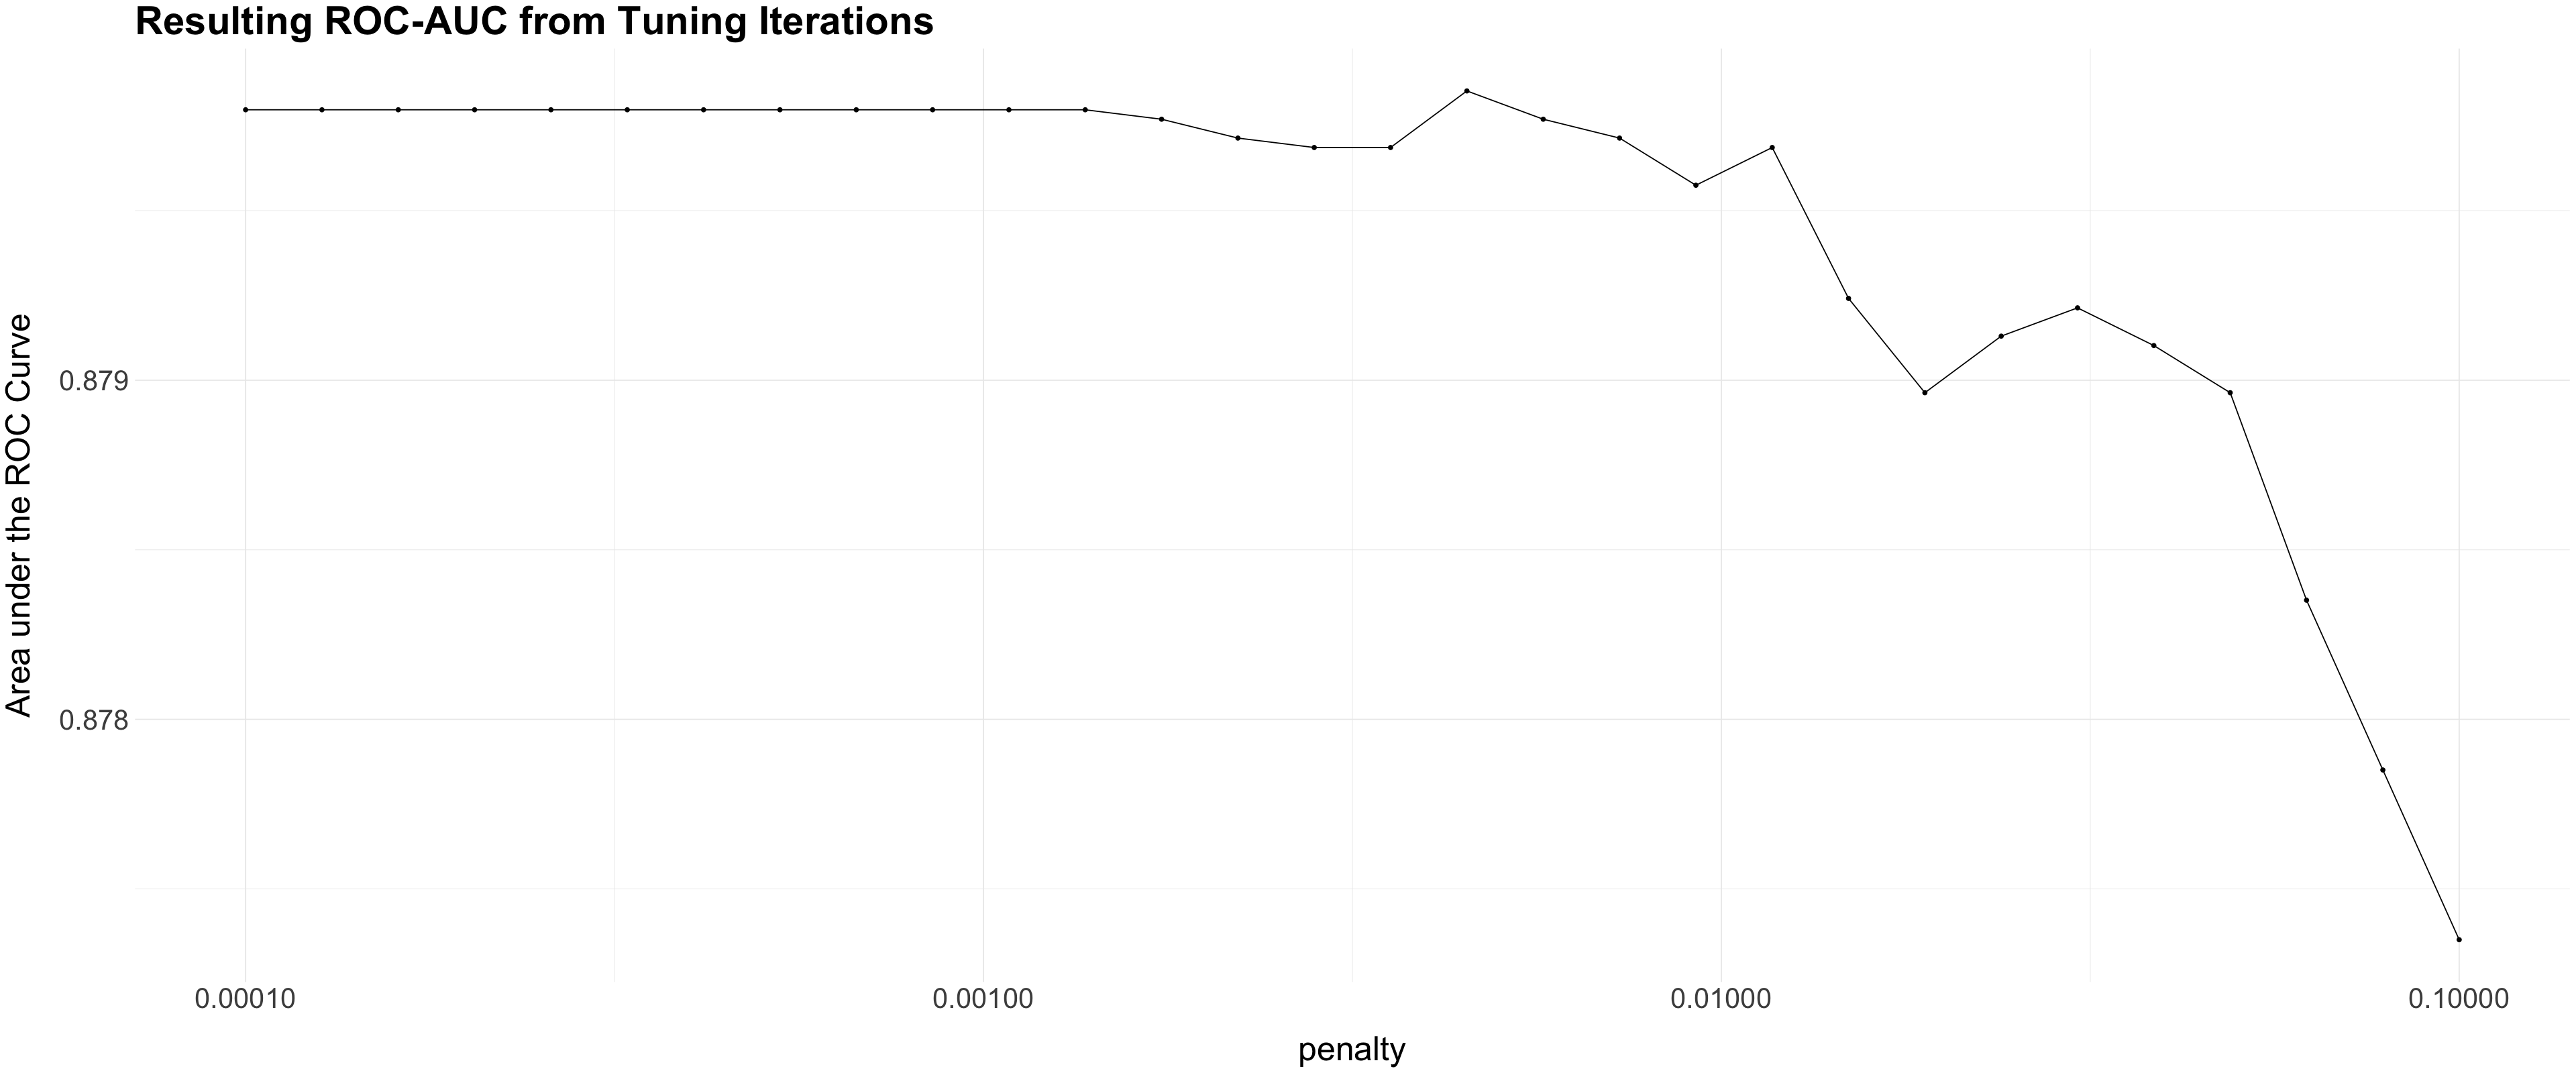
\includegraphics[width=8cm]{_assets/log-reg-plots/log_reg__tuning-plot-roc-curve-1.png}
\end{center}

For our logistic regression model, we also tested an iteration of the model that trained on a randomly oversampled test set, using the methodology set out by ROSE (random oversampling examples), which is a bootstrap method used to generate synthetic samples. In the case of a binary classification of a rare event, oversampling can help to train the model to identify the rare cases more often. Given that an Oscar nominee is only approximately 25 percent of our dataset, we tested ROSE as a potential improvement to the model. However, after testing we found that training on our existing dataset resulted in a higher performing model.

Next, we compared the logistic regression model’s insights to that of our trained random forest, and commented on any similar findings between the two. Insights from both the random forest model and the logistic regression model will be deemed useful to a producer looking to achieve critical acclaim. Therefore, we conclude this methodology section with a brief overview of the methods we used to compare the similarities and differences between our two classification models. Although we do not hypothesize drastic differences in predictive power, we did evaluate and compare the overall performance of each model before examining any key insights. We compared a variety of performance metrics to evaluate the relative predictive power for both models. The performance metrics we used for these two binary classifiers were:

\begin{enumerate}
\item Overall classification accuracy
\item Area under the ROC and Precision/Recall curve 
\item Precision
\item Recall 
\end{enumerate}

In our case, precision is the proportion of predicted Oscar nominees that are actually Oscar nominees. Recall, on the other hand, refers to the proportion of Oscar nominees correctly classified by the model. That is, 

$$\text{precision} = \frac{\text{true Oscar nominees}}{\text{predicted Oscar nominees}}$$
and 
$$\text{recall} = \frac{\text{true Oscar nominees}}{\text{actual Oscar nominees}}$$

In general, higher precision implies that the model returns more relevant results, while higher recall implies that the model returns more correctly classified relevant results. Since one comes at the cost of another, it is impossible to maximize both these metrics at the same time. However, we looked to find an acceptable balance point. 

Lastly, while we looked at all four metrics as an indication of our model performance, accuracy should be viewed with caution, as Oscar nominations are a relatively rare event. If, for example, our model simply classified every observation as not an Oscar nominee, we would obtain approximately 75-80\% accuracy because Oscar nominees are limited to about 20-25\% of the dataset. Therefore, we chose to also focus on precision and recall in order to better understand whether our model was accurately capturing trends and patterns among Oscar nominees.

Once we evaluated the relative performance metrics, we compared the feature importance values obtained from the random forest to the variable coefficients in our logistic regression model. Recall that a logistic regression coefficient (associated with a given feature) represents the expected change in the log odds of being classified as an Oscar nominee per unit change in its corresponding feature. Therefore, if a logistic regression coefficient for a given predictor is $\beta_k$ , increasing that predictor by one unit will multiply the odds of being classified as an Oscar nominee by $e^{\beta_k}$. Note, this means that negative coefficients imply that an increase in the corresponding feature will decrease the odds of being classified as an Oscar nominee. Due to its highly interpretable nature, we will gain slightly more insight from the logistic regression model. However, we still compared the coefficients of the logistic regression model to the permutation importance values reported from our random forest classifier. We expect that the coefficients of the logistic regression model support our permutation importance values from our random forest (i.e. variables corresponding to higher coefficients in the logistic regression model also correspond to higher permutation importance values in the random forest).  

\subsection{Finding Movies that are Similar to an Existing Film}

Rather than try to maximize box office profits or maximize the chance for an Oscar, a movie producer’s idea for a movie might be to simply mimic one or more movies that have already been made. If the executive has a movie in mind, a list of several similar movies could go a long way in understanding key plot points, themes, motifs, cinematography styles, etc. for making a new movie. Instead of a movie executive analyzing countless films with few similarities, we created a system to help executives save time. So, given a particular movie, we produced a list of 9 similar movies based on the release year, runtime, IMDb rating, Metacritic rating, budget, gross in the USA, gross worldwide, whether or not the movie was nominated for an Oscar, whether or not the movie won an Oscar, star power, release month, languages, parental guideline rating, genre, director popularity, and company size using a K-Nearest Neighbors algorithm.

K-Nearest Neighbors is a non-parametric supervised training algorithm used to find the K-nearest observations to the one given. In our case, we started with one movie title and calculated the euclidean distance to all other movies in our dataset. The 9 most similar movies had the smallest euclidean distance based on the features above. Typically, a K-Nearest Neighbors algorithm only works with numeric variables, but by dummy coding our categorical variables, we included extra information in the algorithm. Lastly, we replaced missing values in the numeric variables with the variable’s mean. 

\section{Results and Discussion}
\subsection{Model and Maximize Box Office Profits}

Using budget, runtime, genres, content rating, director popularity, movie release period, runtime, company size, star power, and writer popularity as predictor variables, we trained our random forest algorithm. After tuning our hyper-parameters, we found that 1100 trees (bootstrap resamples) with 7 variables randomly sampled as candidates for each split were optimal for our model. Using these parameters in our model achieved the lowest average RMSE and maintained the highest average R-Squared values (averaged over the 10 folds in our cross validation data set). Then, we trained our random forest model with the entirety of our training set using 1100 trees with 7 variables randomly sampled as candidates for each split and attempted to predict the box office profit of the movies in our test data set. The predictions had an RMSE of about 429,496.70 U.S. dollars and an R-Squared of about 0.457. This relatively large R-Squared value indicates that a large proportion of the variation in the box office profit data is explained very well by the predictor variables in our dataset. And given that the standard deviation of the box office profit in our data is about 229,317,065 U.S. dollars, our model’s reported RMSE is relatively low. In fact, the reported RMSE is less than 0.2\% of the standard deviation in our box office profit data.

Since our random forest has demonstrated strong predictive power, we move on to discuss the key insights it provides, and how these insights can be leveraged by a movie producer. We calculated and plotted the feature importances using the Permutation Importance method described in the \textit{Methodology} section. Below is the plot of the ordered importance values we found. 

\begin{center}
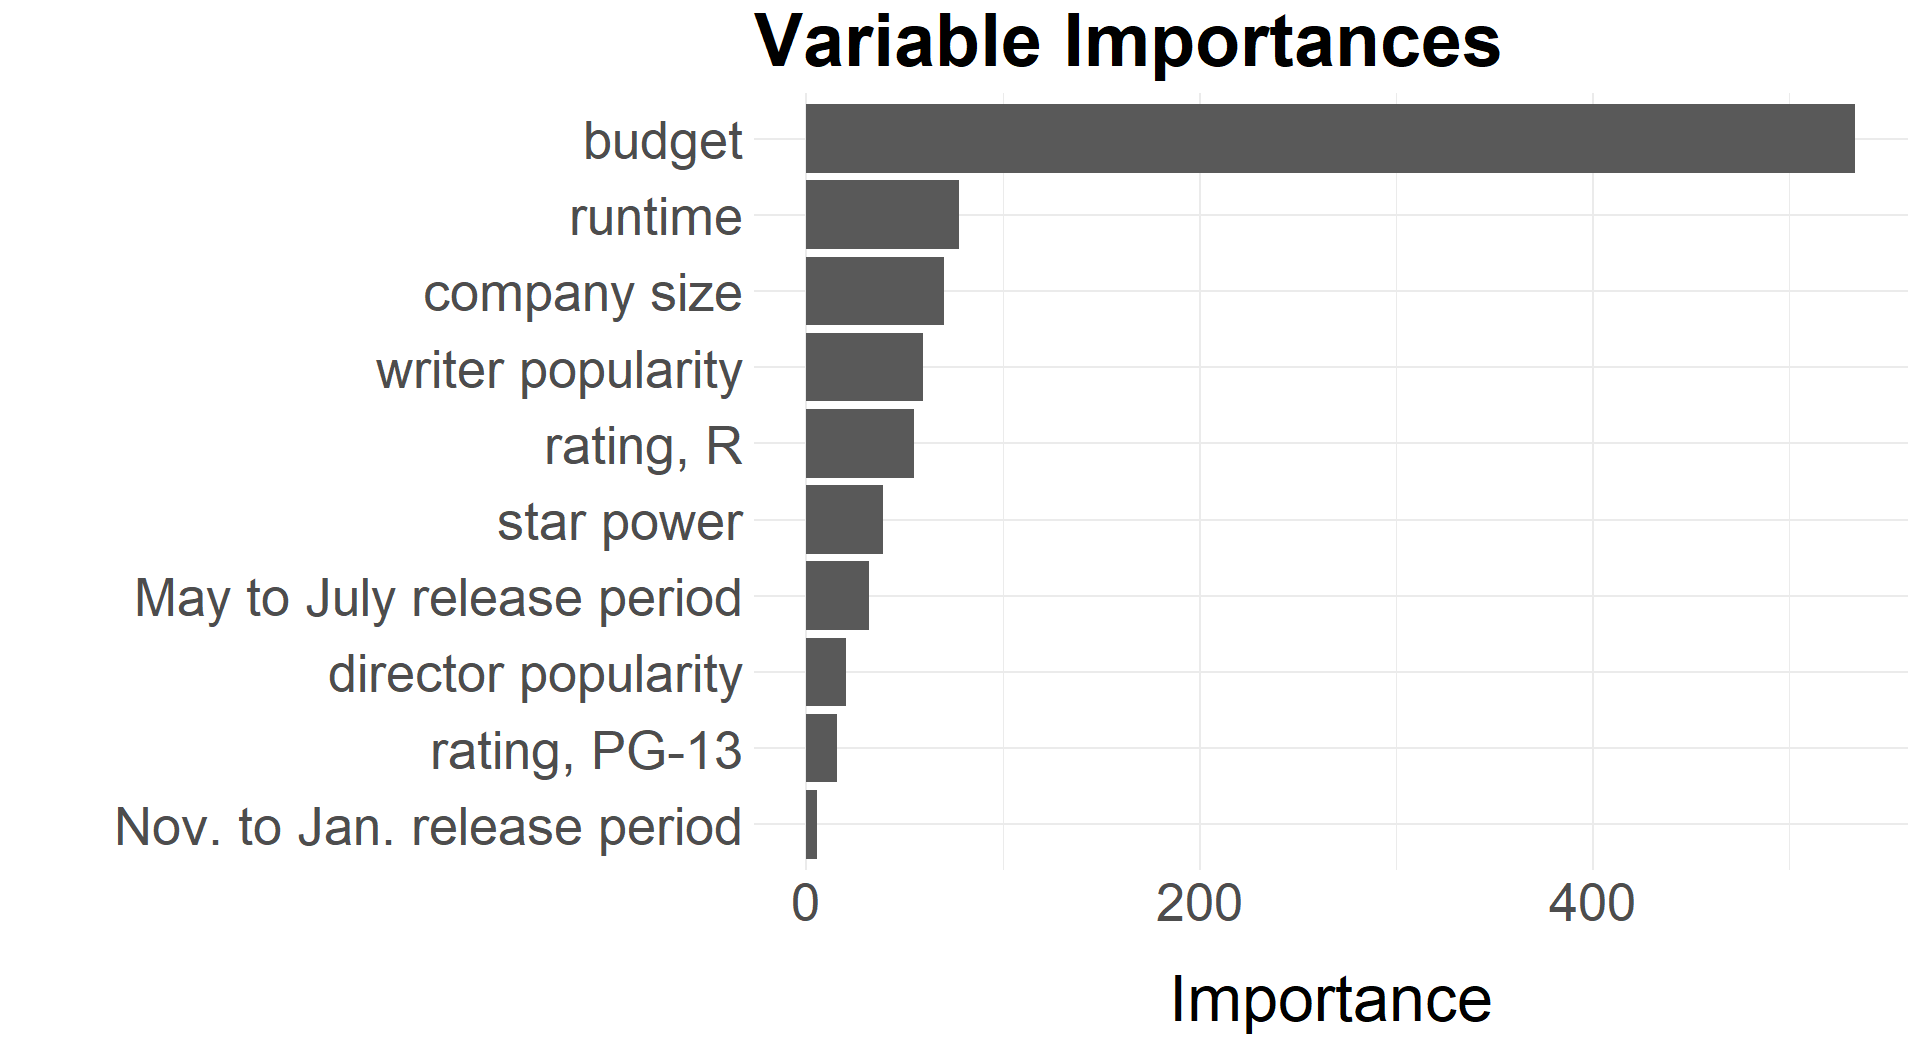
\includegraphics[width=8cm]{_assets/predictive_analysis/variable_importance_rf_bop.png}
\end{center}

Not only can we see that budget has the highest reported feature importance, it is substantially higher than any other predictor variable in our training set. Therefore, our model indicates that budget demonstrates greater ability to predict box office profit than all other variables in the training set. Additionally, we can see above that runtime, company size, writer popularity, and R ratings, demonstrate relatively strong predictive power over the other variables. Earlier, we saw that budget, runtime, and company size are positively correlated with box office profits, thus supporting the feature importance scores from our random forest model. 

We now compare the results of our random forest to that of a standard linear regression model. Using a similar set of predictor variables from the training data we used for the random forest model, we generated our linear regression model. We applied this model to the test data and observed an RMSE of about 549,498.70 U.S. dollars and an R-Squared of about 0.365. Although these values are not as strong as they were with the random forest, they still indicate that our linear model is a good fit, and can provide additional insights. We provide a tabled summary of our linear model here:

\begin{table}[ht]
\centering
\begin{tabular}{llr}
  \hline
Coefficients & Estimate & Std. Error & P-Value \\ 
  \hline
(Intercept) & 93.9317 & 1.2583 & 2e-16 \\
budget_adj & 16.7476 & 0.7439 & 2e-16 \\
runtime & 2.3632 & 0.6835 & 0.000557 \\
dir_pop_fac & -0.1901 & 0.6980 & 0.785423 \\  
release_periodfeb_to_apr & -0.5301 & 1.7848 & 0.766505 \\  
release_periodmay_to_jul & 8.4182 & 1.7899 & 2.74e-06 \\
release_periodnov_to_jan & 4.4887 & 1.7222 & 0.009221 \\
co_size & 4.1257 & 0.6689 & 8.42e-10 \\ 
star_power & 0.1404 & 0.6969 & 0.840306 \\   
wr_pop & 3.2517 & 0.6485 & 5.80e-07 \\
   \hline
\end{tabular}
\caption{Summary of Box-Office Profit Linear Model} 
\label{tab:lm_sum}
\end{table}



Note that before we actually fit our linear model, we normalized the numeric data to have a mean of 0 and a standard deviation of 1, so we can interpret the regression coefficients of the \textit{numeric} predictors with ease. Clearly, the largest regression coefficient from the numeric variables in the linear model is budget. The budget feature coefficient is approximately 4 times larger than the next largest coefficient in our model, and its extremely low p-value indicates that it is highly significant. Once again, this emphasizes the importance of the budget predictor, and supports our findings from the feature importances of the random forest. Additionally, since we know this coefficient is positive, we can expect that an increase in budget corresponds to an increase in box office profit. From the table above, we can also see that the next two largest regression coefficients from the numeric variables are company size and writer popularity. While the coefficient for company size is slightly larger than the coefficient for writer popularity, both have very low p-values, indicating that each of them are certainly significant. Given that company size and writer popularity ranked 3rd and 4th on the feature importance list from our random forest model, their large coefficients and low p-values support the findings from our random forest. Since both of these coefficients are positive, we can expect that an increase in company size and writer popularity leads to an increase in box office profits. 

A major difference in the insights from the linear regression model and the random forest model is the level of importance placed on the runtime predictor variable. As we can see from our above tables and plots, the linear model does not place as much importance on the runtime variable as the random forest model does. Conversely, the random forest seems to place less importance on the May-July release period, but the variable’s relatively low p-value in the linear model seems to indicate a high importance on this variable. Given that the random forest model has slightly better predictive power than the linear model (comparing the RMSE and R-Squared), we believe that runtime should remain as one of the more important features, and the May-July release period should remain as a less valued predictor variable. 

In conclusion, our two box office profit models certainly agree that budget is the most important predictor variable in our dataset, and that both company size and writer popularity are useful features when predicting box office profit. In addition, our random forest model places an emphasis on the importance of runtime in determining box office profits. Not only did our models provide us with the magnitude of importance, but we also saw from both the plots and the signs of the linear regression coefficients that if we increase the budget, company size, writer popularity, or runtime of a movie, we would expect an increase in box office profit. Therefore, these are the variables a producer should place extra emphasis on when developing a new movie. 

\subsection{Model and Maximize Chances of an Academy Award Nomination}

Using budget, runtime, genres, content rating, director popularity, movie release period, runtime, company size, star power, and writer popularity as predictor variables, we trained our random forest binary classification model. For this model, we found that 1250 trees (bootstrap resamples) with 7 variables randomly sampled as candidates for each split were optimal for our model. Using these parameters in our binary classification model achieved the highest accuracy and maintained a relatively large average area under the ROC curve. Then, we trained our random forest model with the entirety of our training set using 1250 trees with 7 variables randomly sampled as candidates for each split and attempted to predict the movies that were Oscar nominees in our test data set. Approximately 80.4\% of the predictions were found to be correct, and the area under the ROC curve was at 0.80. 

Using the same predictor variables, we then trained our logistic regression model as well. After tuning our threshold and penalty terms, we attempted to predict the movies that were Oscar nominees in the test data set. This time, we observed an accuracy of about 87.6\%, and an area under the ROC curve of about 0.88.

The accuracy and ROC curve metrics from both the random forest and the logistic regression model indicate that our logistic regression model has substantial predictive power. However, note that only about 25\% of films in our dataset were Oscar nominated. Since the proportion of Oscar nominated movies is not very high, we compare the relative predictive power of our two models using their precision and recall. 

\begin{table}[ht]
\centering
\begin{tabular}{llr}
  \hline
Model Type & Precision & Recall \\ 
  \hline
Random Forest & 0.685 & 0.420 \\
Logistic Regression & 0.702 & 0.431 \\
   \hline
\end{tabular}
\caption{Summary of Box-Office Profit Linear Model} 
\label{tab:lm_sum}
\end{table}



We can see above that both models have fairly similar precision and recall values. Even though our recall is only about 42-43\%, approximately 70\% of predicted Oscar nominees are actually Oscar nominees for both models. These metrics, including the overall accuracy and area of the ROC curve, indicate that the random forest and the logistic regression model both fit the data well and demonstrate relatively strong predictive power. From the random forest model, we find that runtime and budget are among the most important variables.

\begin{center}
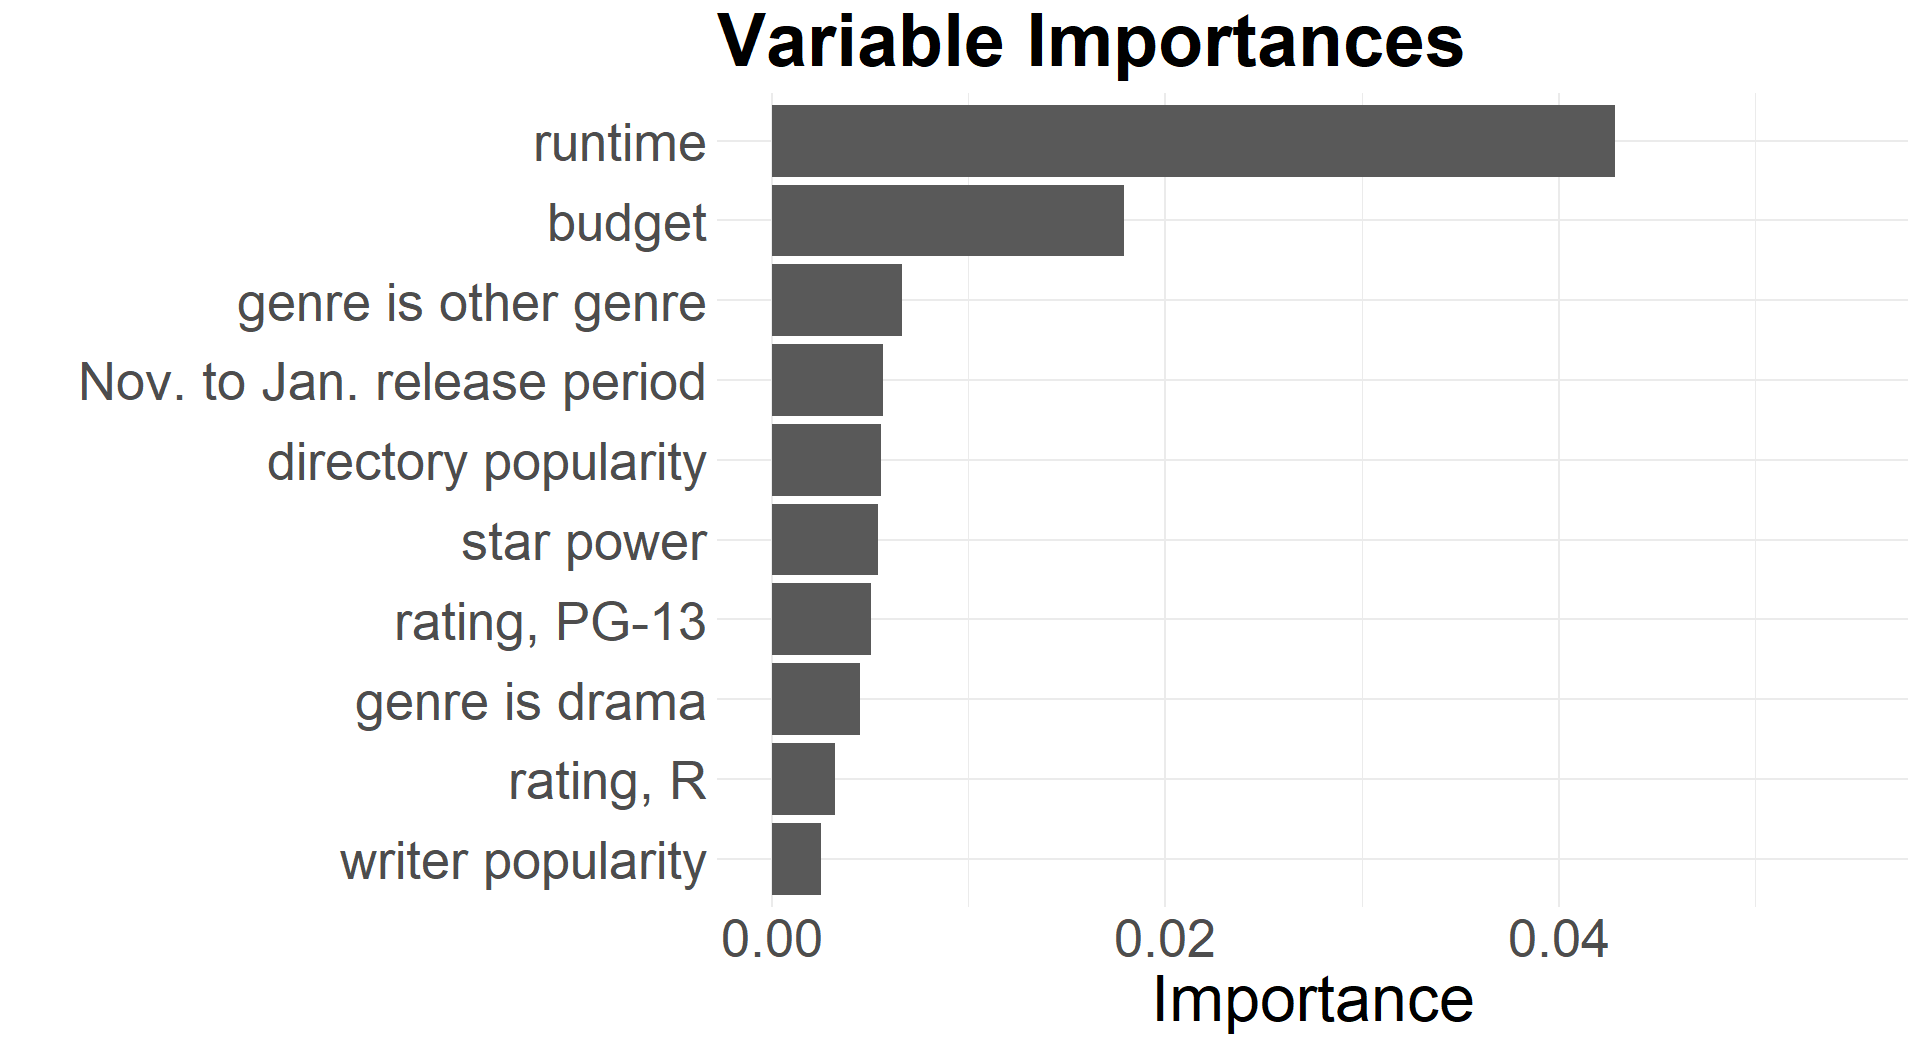
\includegraphics[width=8cm]{_assets/predictive_analysis/variable_importance_rf_osc_nom.png}
\hspace{1cm}
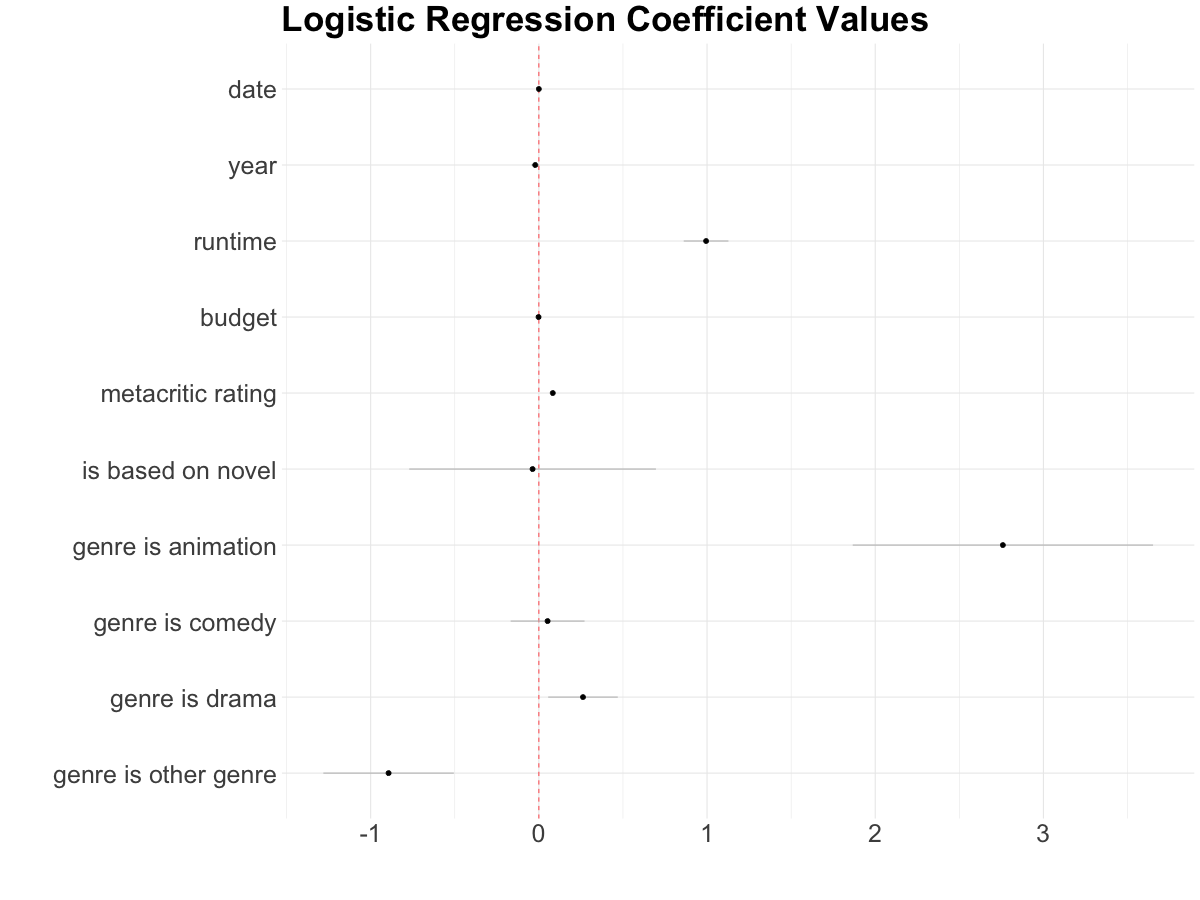
\includegraphics[width=8cm]{_assets/log-reg-plots/dwplot.png}
\end{center}

However, we also see from our importance plot that the uncommon genres and Nov. to Jan. release period demonstrate relatively strong predictive importance as well. Earlier we saw that runtime, budget, and the November-to-January release period are all positively correlated with Oscar nomination status, thus supporting their feature importance scores from our random forest classifier. Similarly, the Oscar Nominees by Genres figure demonstrates support for our random forest’s feature importance scores as well. We can see that drama films, and non-standard genre films have a noticeably higher Oscar nominee proportion, indicating positive correlation with Oscar nomination status. 

Using the logistic regression to further corroborate these correlative findings, we see that both runtime and budget are also among the most highly correlated variables in regards to increasing the chances of an Oscar nomination, with every 60 minutes correlating with a 4\% increase in the odds of an Oscar nomination. 

While the random forest shows budget to be the second most important variable from all inputs feeding into the model, the logistic regression found budget to be of very little impact, with an odds ratio of close to 1 indicating that a unit increase in budget had neither a large negative nor positive effect. This may be due to the fact that a random forest can deal with non-linear variables better than a logistic regression can. When comparing budget to Metacritic ratings (which we can assume to be highly correlated with an Oscar nomination), we find that there is a non-linear relationship between budget and Metacritic rating. 

\begin{center}
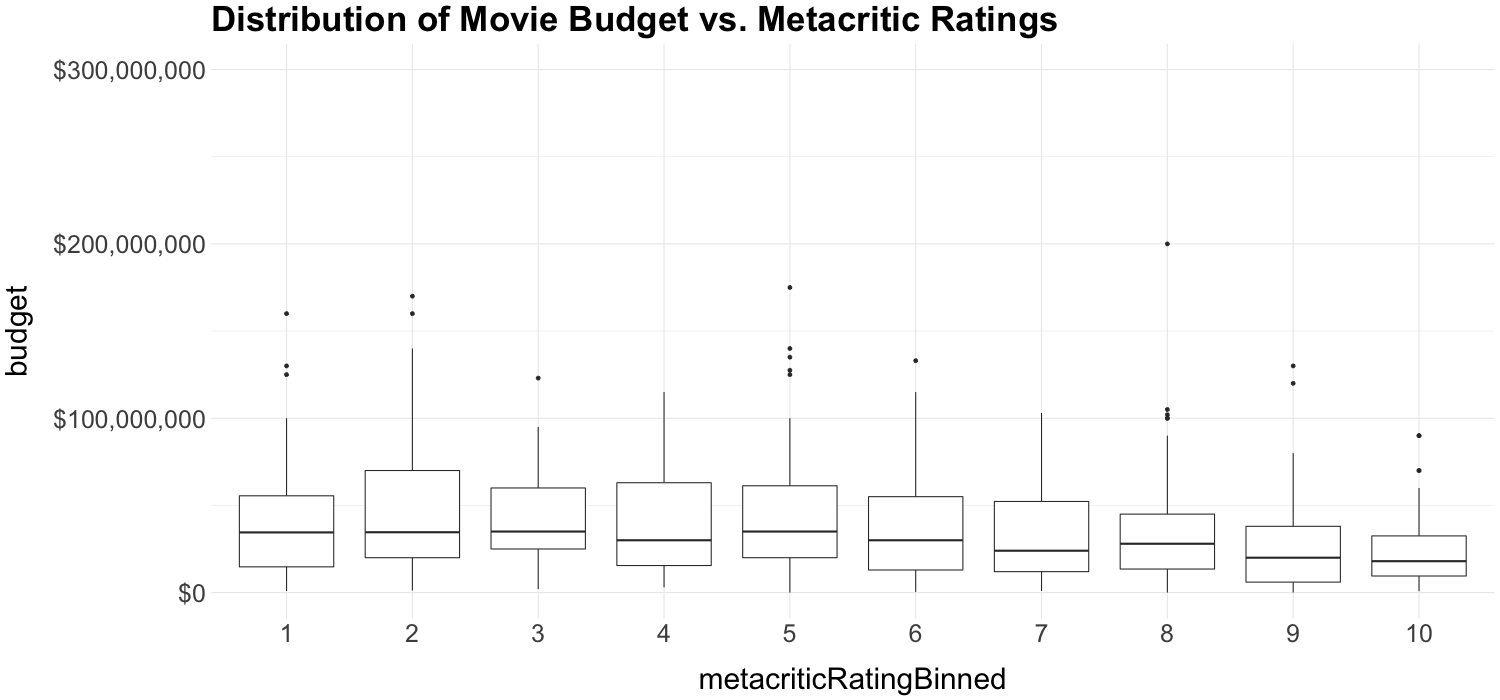
\includegraphics[width=8cm]{_assets/_eda/eda__boxplot_budget_vs_metacritic_binned.png}
\end{center}

Some hypotheses as to why this occurs may be due to large blockbuster films such as Marvel movies having a large budget and no intention of winning Oscars while smaller, art house films, may limit themselves to a smaller budget with more of a focus on the artistry of film making that attracts the Oscar nominating committee. The random forest was better suited to identifying this non-linear, correlative relationship than the logistic regression model.

Additionally, we looked at genres that were more likely to be correlated with an Oscar nomination. Both the random forest and the logistic regression found that Drama films were among the most influential (from the variable importance derived from the random forest) and positively correlated (derived from the coefficients from the logistic regression) with an Oscar nomination when compared to other genres. In fact, if comparing two movies with similar budgets and Metacritic ratings, we found that a Drama film was approximately 1.6 times more likely to be nominated for an Oscar than a Comedy film.

\subsection{Finding Movies that are Similar to an Existing Film}

Lastly, we are going to provide a few examples showcasing our movie recommendation algorithm and the insights we gain from a movie’s nearest neighbors.  

Let’s say a producer wants to mimic any high grossing movie. Star Wars: Episode VII - The Force Awakens (2015) has the highest US Gross among all movies in our dataset. We recommend the producer work with Disney as other Disney movies are the most similar to Star Wars: Episode VII - The Force Awakens (2015). Among its 50 nearest movies, the most common word from the plot summary is “world”. This makes sense because the Star Wars movies and Marvel movies focus on a group of heroes trying to save the world from an evil being. Thus, it also makes sense that the most common keyword from these movies is superhero. If a movie producer is trying to mimic Star Wars, we recommend the executive make a superhero action or adventure movie. 

\begin{center}
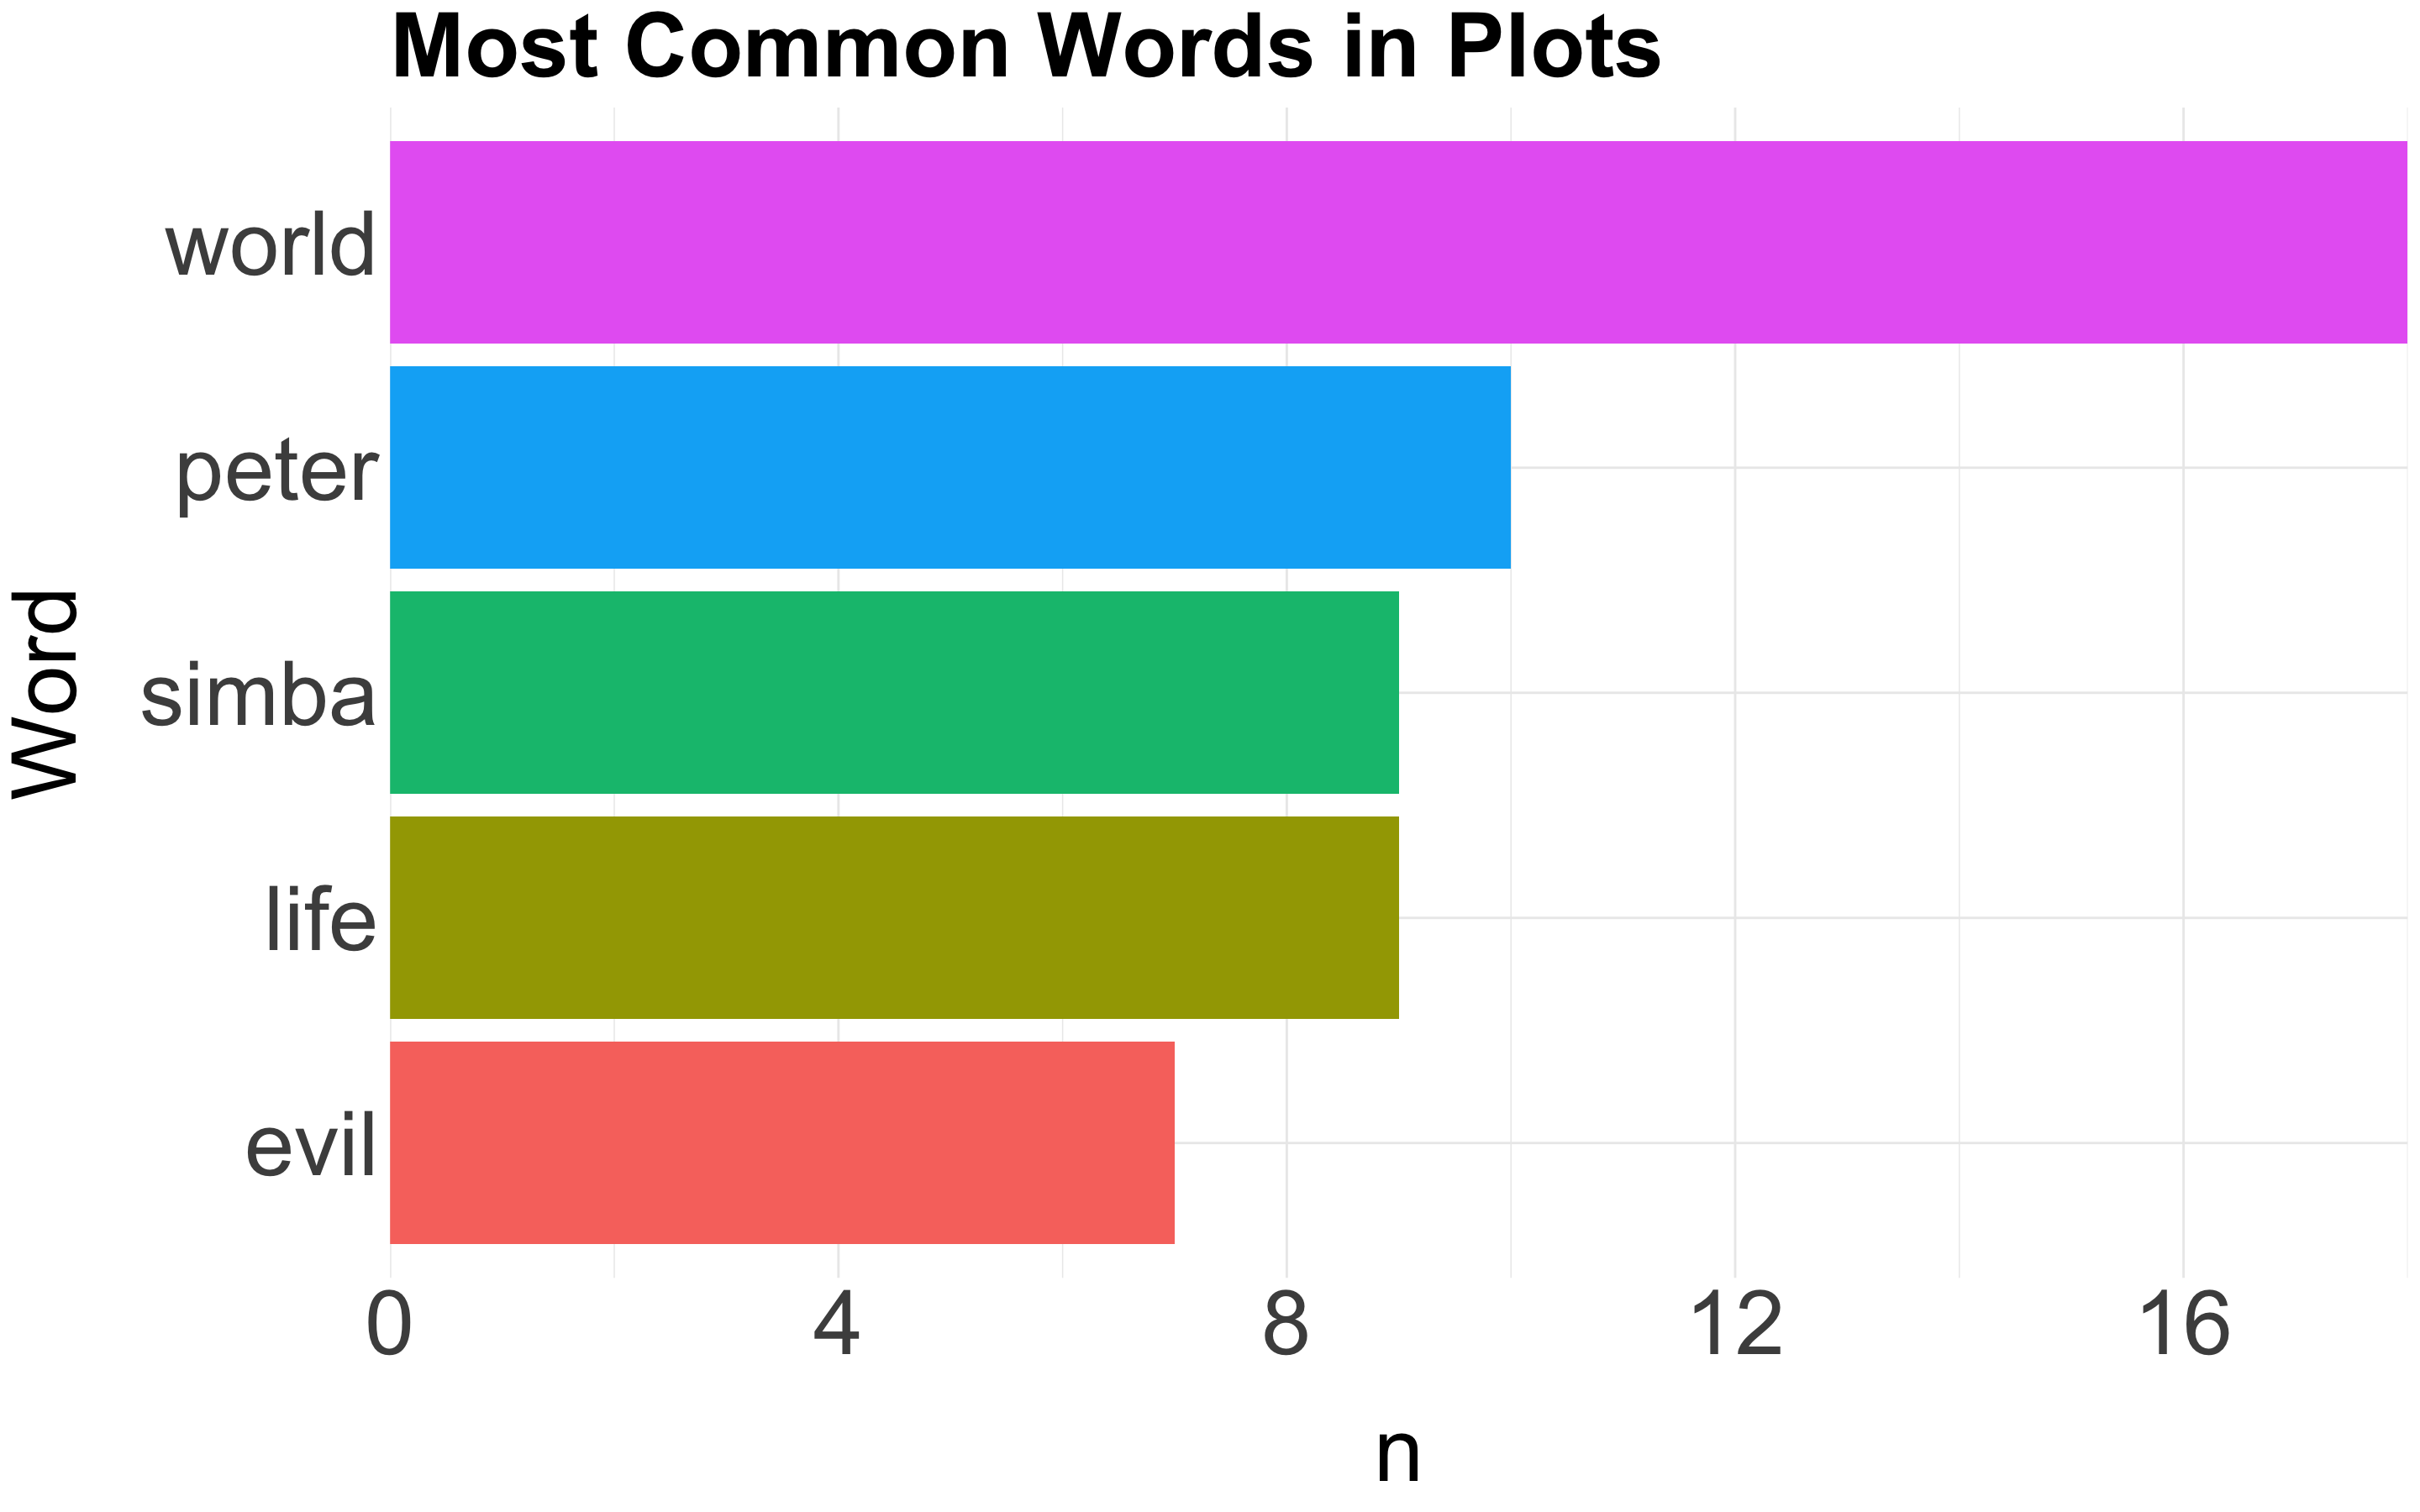
\includegraphics[width=8cm]{_assets/_assets_knn/star_wars_common_words.png}
\hspace{1cm}
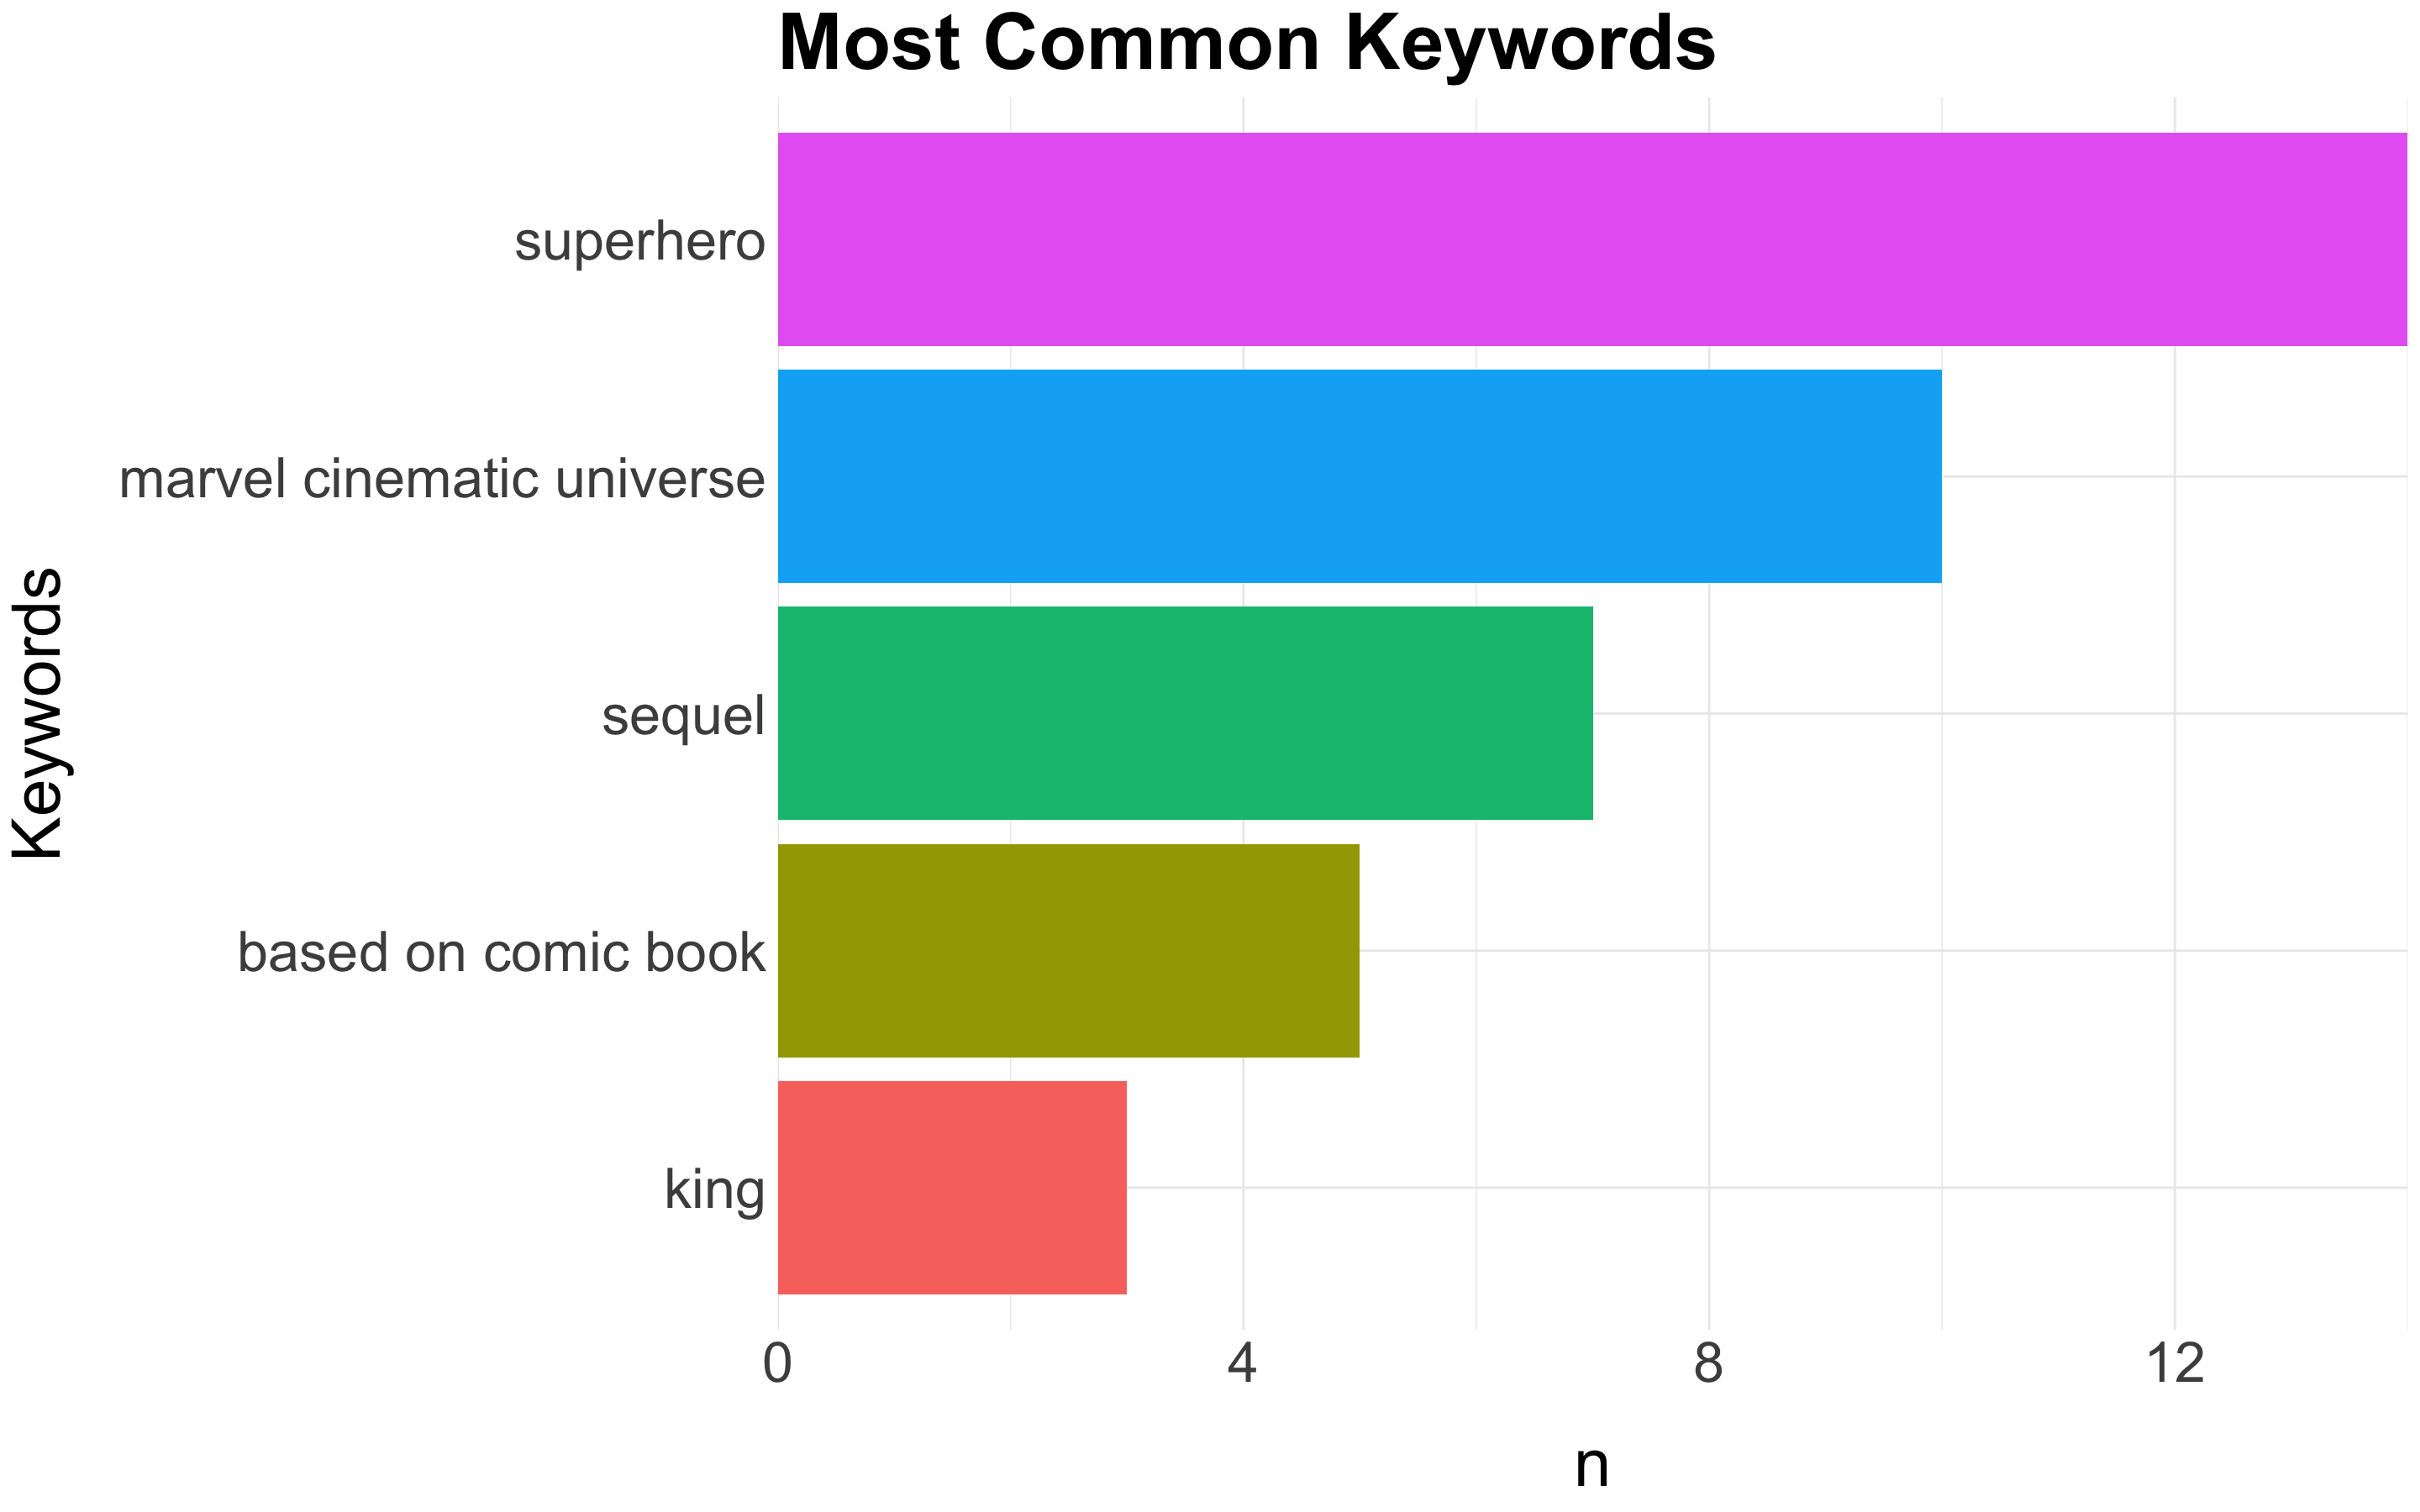
\includegraphics[width=8cm]{_assets/_assets_knn/star_wars_common_keywords.png}
% latex table generated in R 4.2.0 by xtable 1.8-4 package
% Sat Jun  4 12:47:09 2022
\begin{table}[H]
\centering
\begin{tabular}{llr}
  \hline
Full Title & Gross USA \$ & Oscar Won \\ 
  \hline
Star Wars: Episode VII - The Force Awakens (2015) & 936,662,225 &   0 \\ 
  Spider-Man: No Way Home (2021) & 804,617,772 &   0 \\ 
  Avengers: Infinity War (2018) & 678,815,482 &   0 \\ 
  Avengers: Endgame (2019) & 858,373,000 &   0 \\ 
  Incredibles 2 (2018) & 608,581,744 &   0 \\ 
  Star Wars: Episode VIII - The Last Jedi (2017) & 620,181,382 &   0 \\ 
  Black Panther (2018) & 700,426,566 &   1 \\ 
  The Lion King (2019) & 543,638,043 &   0 \\ 
  Jurassic World (2015) & 653,406,625 &   0 \\ 
  Avatar (2009) & 760,507,625 &   1 \\ 
   \hline
\end{tabular}
\caption{The Nearest Movies to Star Wars: Episode VII - The Force Awakens (2015)} 
\end{table}


\end{center}

Instead of a producer focusing on high grossing action and adventure movies, let’s say a producer wants to mimic an Oscar winning film such as “The Godfather (1972)”. The Godfather (1972) has the highest Metacritic and IMDb rating among movies that won an Oscar. We suggest the producer analyze other 1970s crime films such as The Godfather: Part II (1974), Midnight Express (1978), Taxi Driver (1976), and Chinatown (1974) because these films are included in the Godfather’s 9 nearest movies. Additionally, these four movies all won an Oscar and three out of the four had a Metacritic rating of at least 90. Since the majority of the nearest neighbors are drama and crime films, we also suggest the new movie include murder, revenge, and organized crime.

\begin{center}
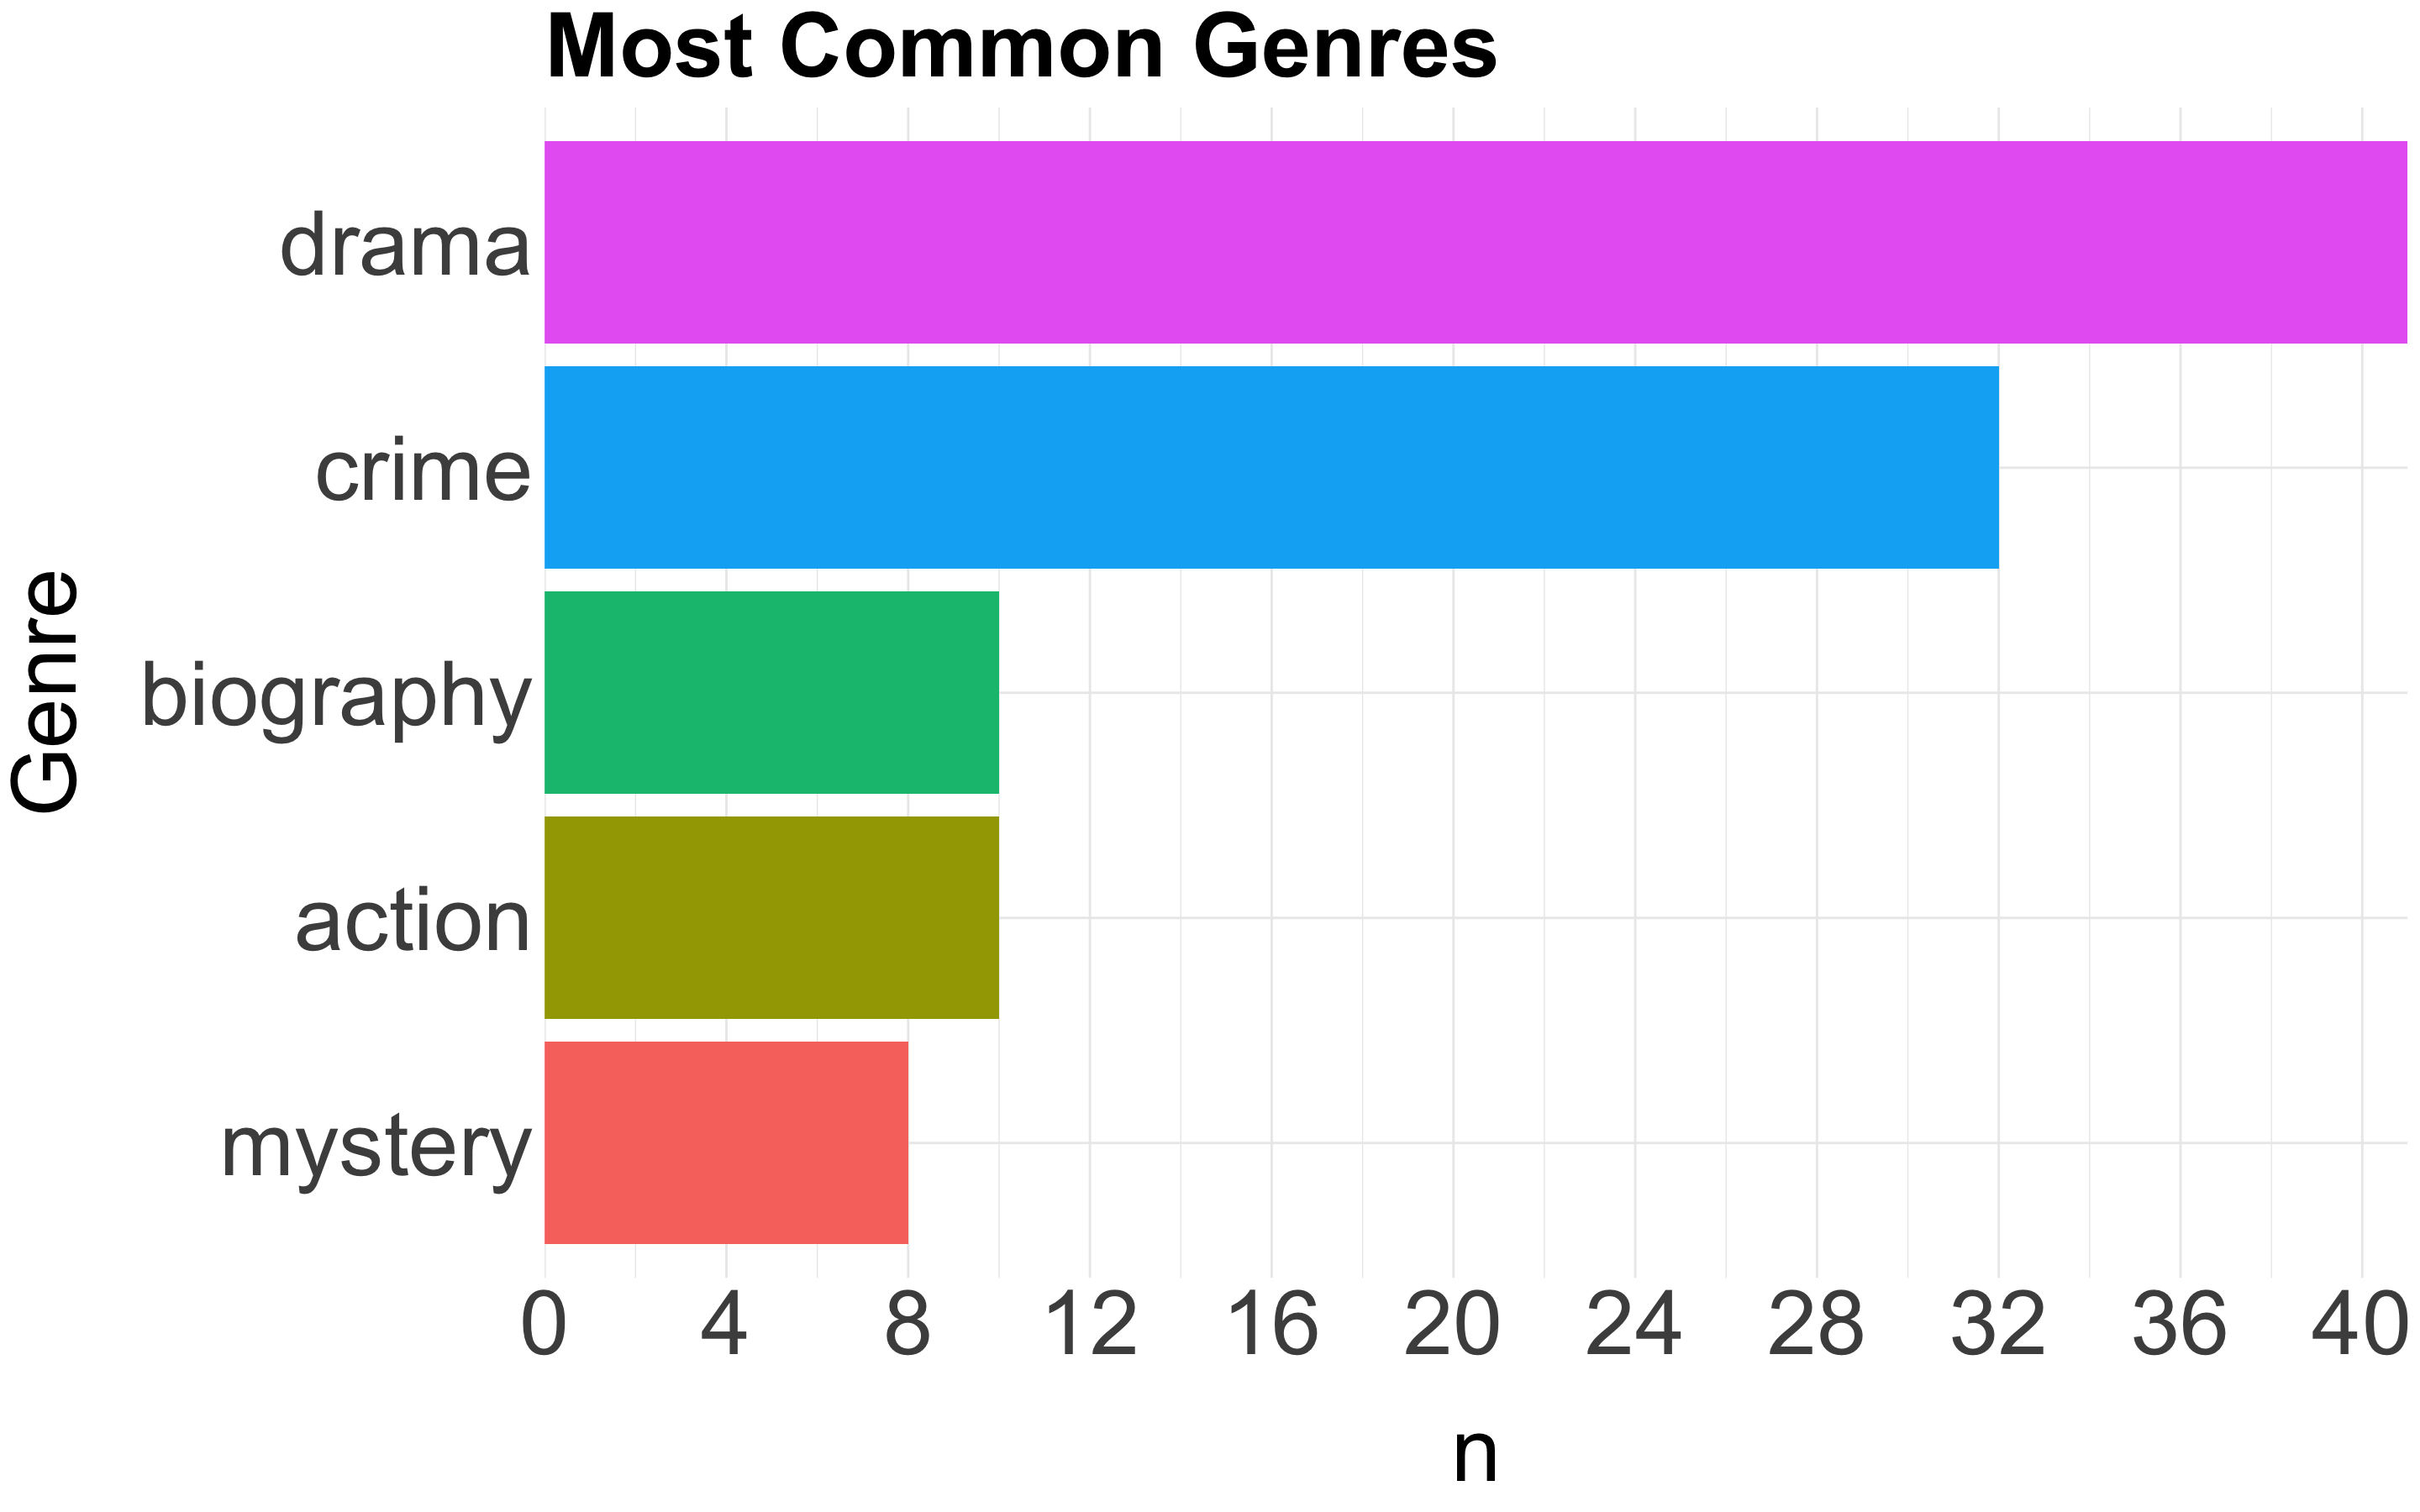
\includegraphics[width=8cm]{_assets/_assets_knn/godfather_common_genres.png}
\hspace{1cm}
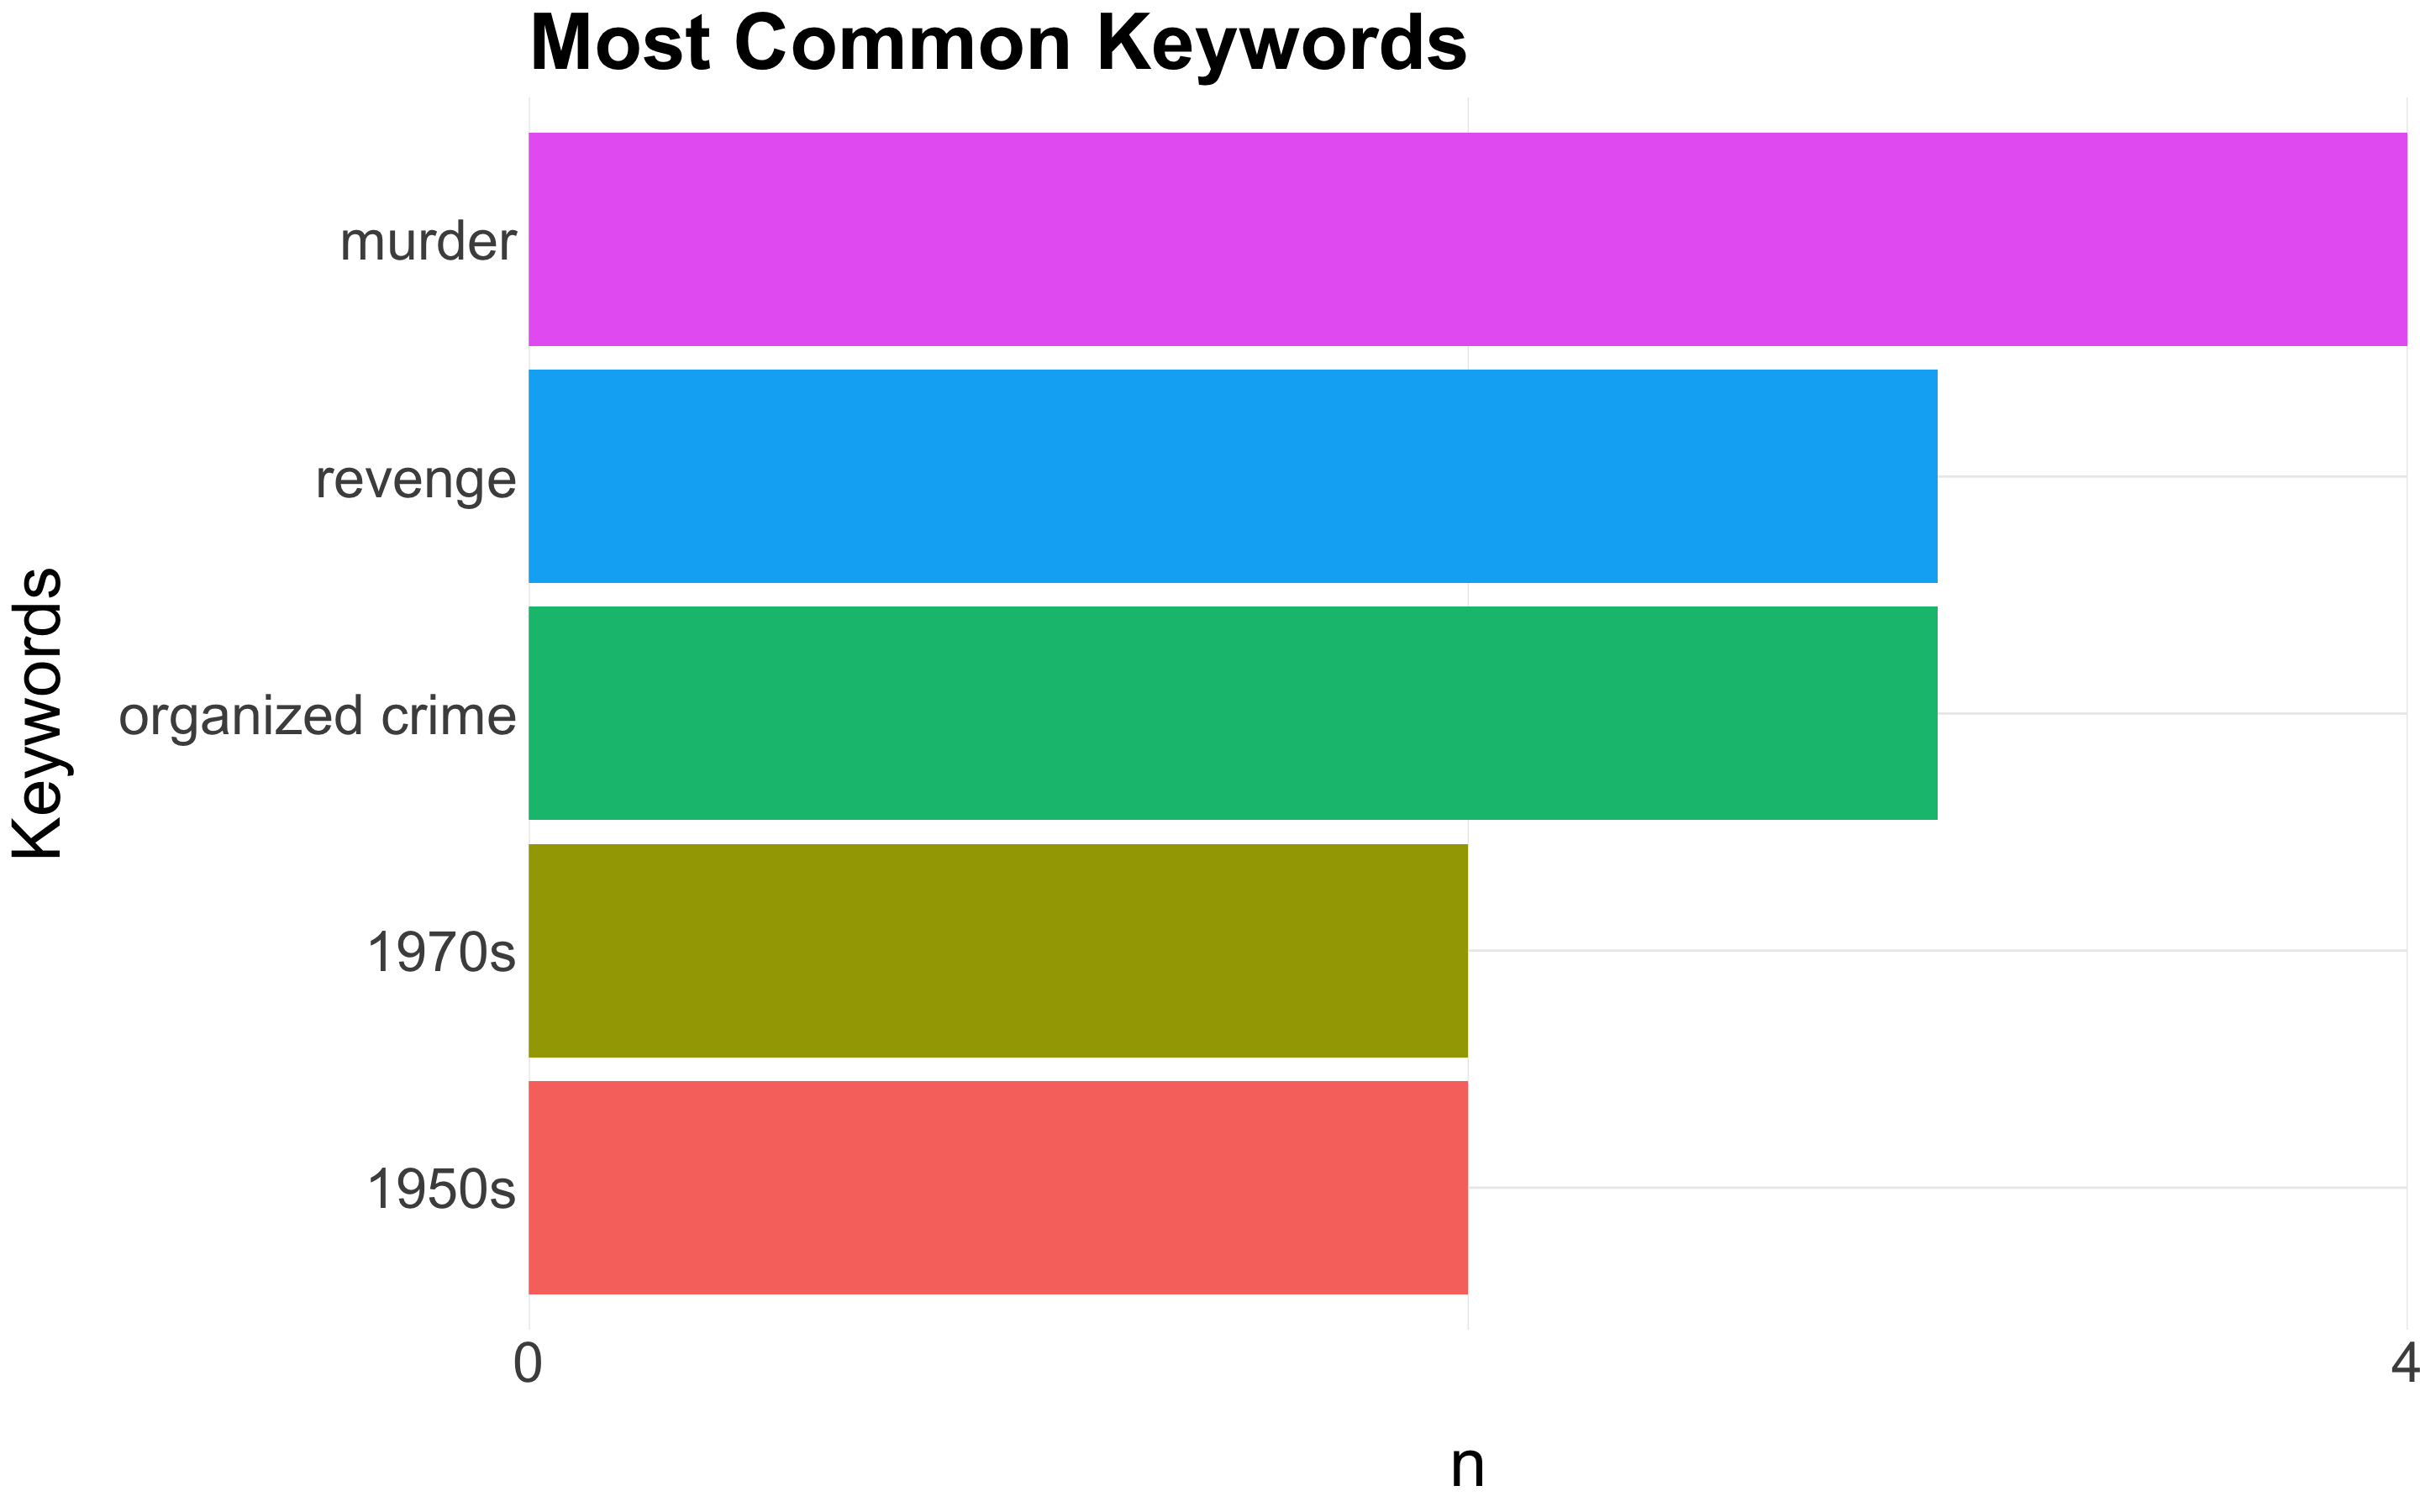
\includegraphics[width=8cm]{_assets/_assets_knn/godfather_common_keywords.png}
% latex table generated in R 4.2.0 by xtable 1.8-4 package
% Sat Jun  4 12:47:33 2022
\begin{table}[H]
\centering
\begin{tabular}{lrrr}
  \hline
Full Title & Metacritic Rating & IMDb Rating & Oscar Won \\ 
  \hline
The Godfather (1972) & 100.00 & 9.20 &   1 \\ 
  Goodfellas (1990) & 90.00 & 8.70 &   1 \\ 
  The Godfather: Part II (1974) & 90.00 & 9.00 &   1 \\ 
  The Girl with the Dragon Tattoo (2011) & 71.00 & 7.80 &   1 \\ 
  Midnight Express (1978) & 59.00 & 7.50 &   1 \\ 
  Pulp Fiction (1994) & 94.00 & 8.90 &   1 \\ 
  Taxi Driver (1976) & 94.00 & 8.30 &   0 \\ 
  Schindlers List (1993) & 94.00 & 9.00 &   1 \\ 
  Chinatown (1974) & 92.00 & 8.20 &   1 \\ 
  Scarface (1983) & 65.00 & 8.30 &   0 \\ 
   \hline
\end{tabular}
\caption{The Nearest Movies to The Godfather (1972)} 
\end{table}


\end{center}

Forrest Gump (1994) is widely considered a classic American film starring Tom Hanks. Let’s say a producer hopes to mimic this movie and wants Tom Hanks to star as the main character. For the sake of argument, let’s also say Tom Hanks is not available for this role, so the producer needs to find a different actor. We suggest the producer look to “The Great Gatsby (2013)”, “A Beautiful Mind (2001)”, or “Cinderella Man (2005)” for inspiration. The movie producer can cast another star actor such as Leonardo DiCaprio or Russell Crowe because they are featured in these films. With these particular actors, we suggest the new movie be a drama or romance film with themes related to life, time, and love.

\begin{center}
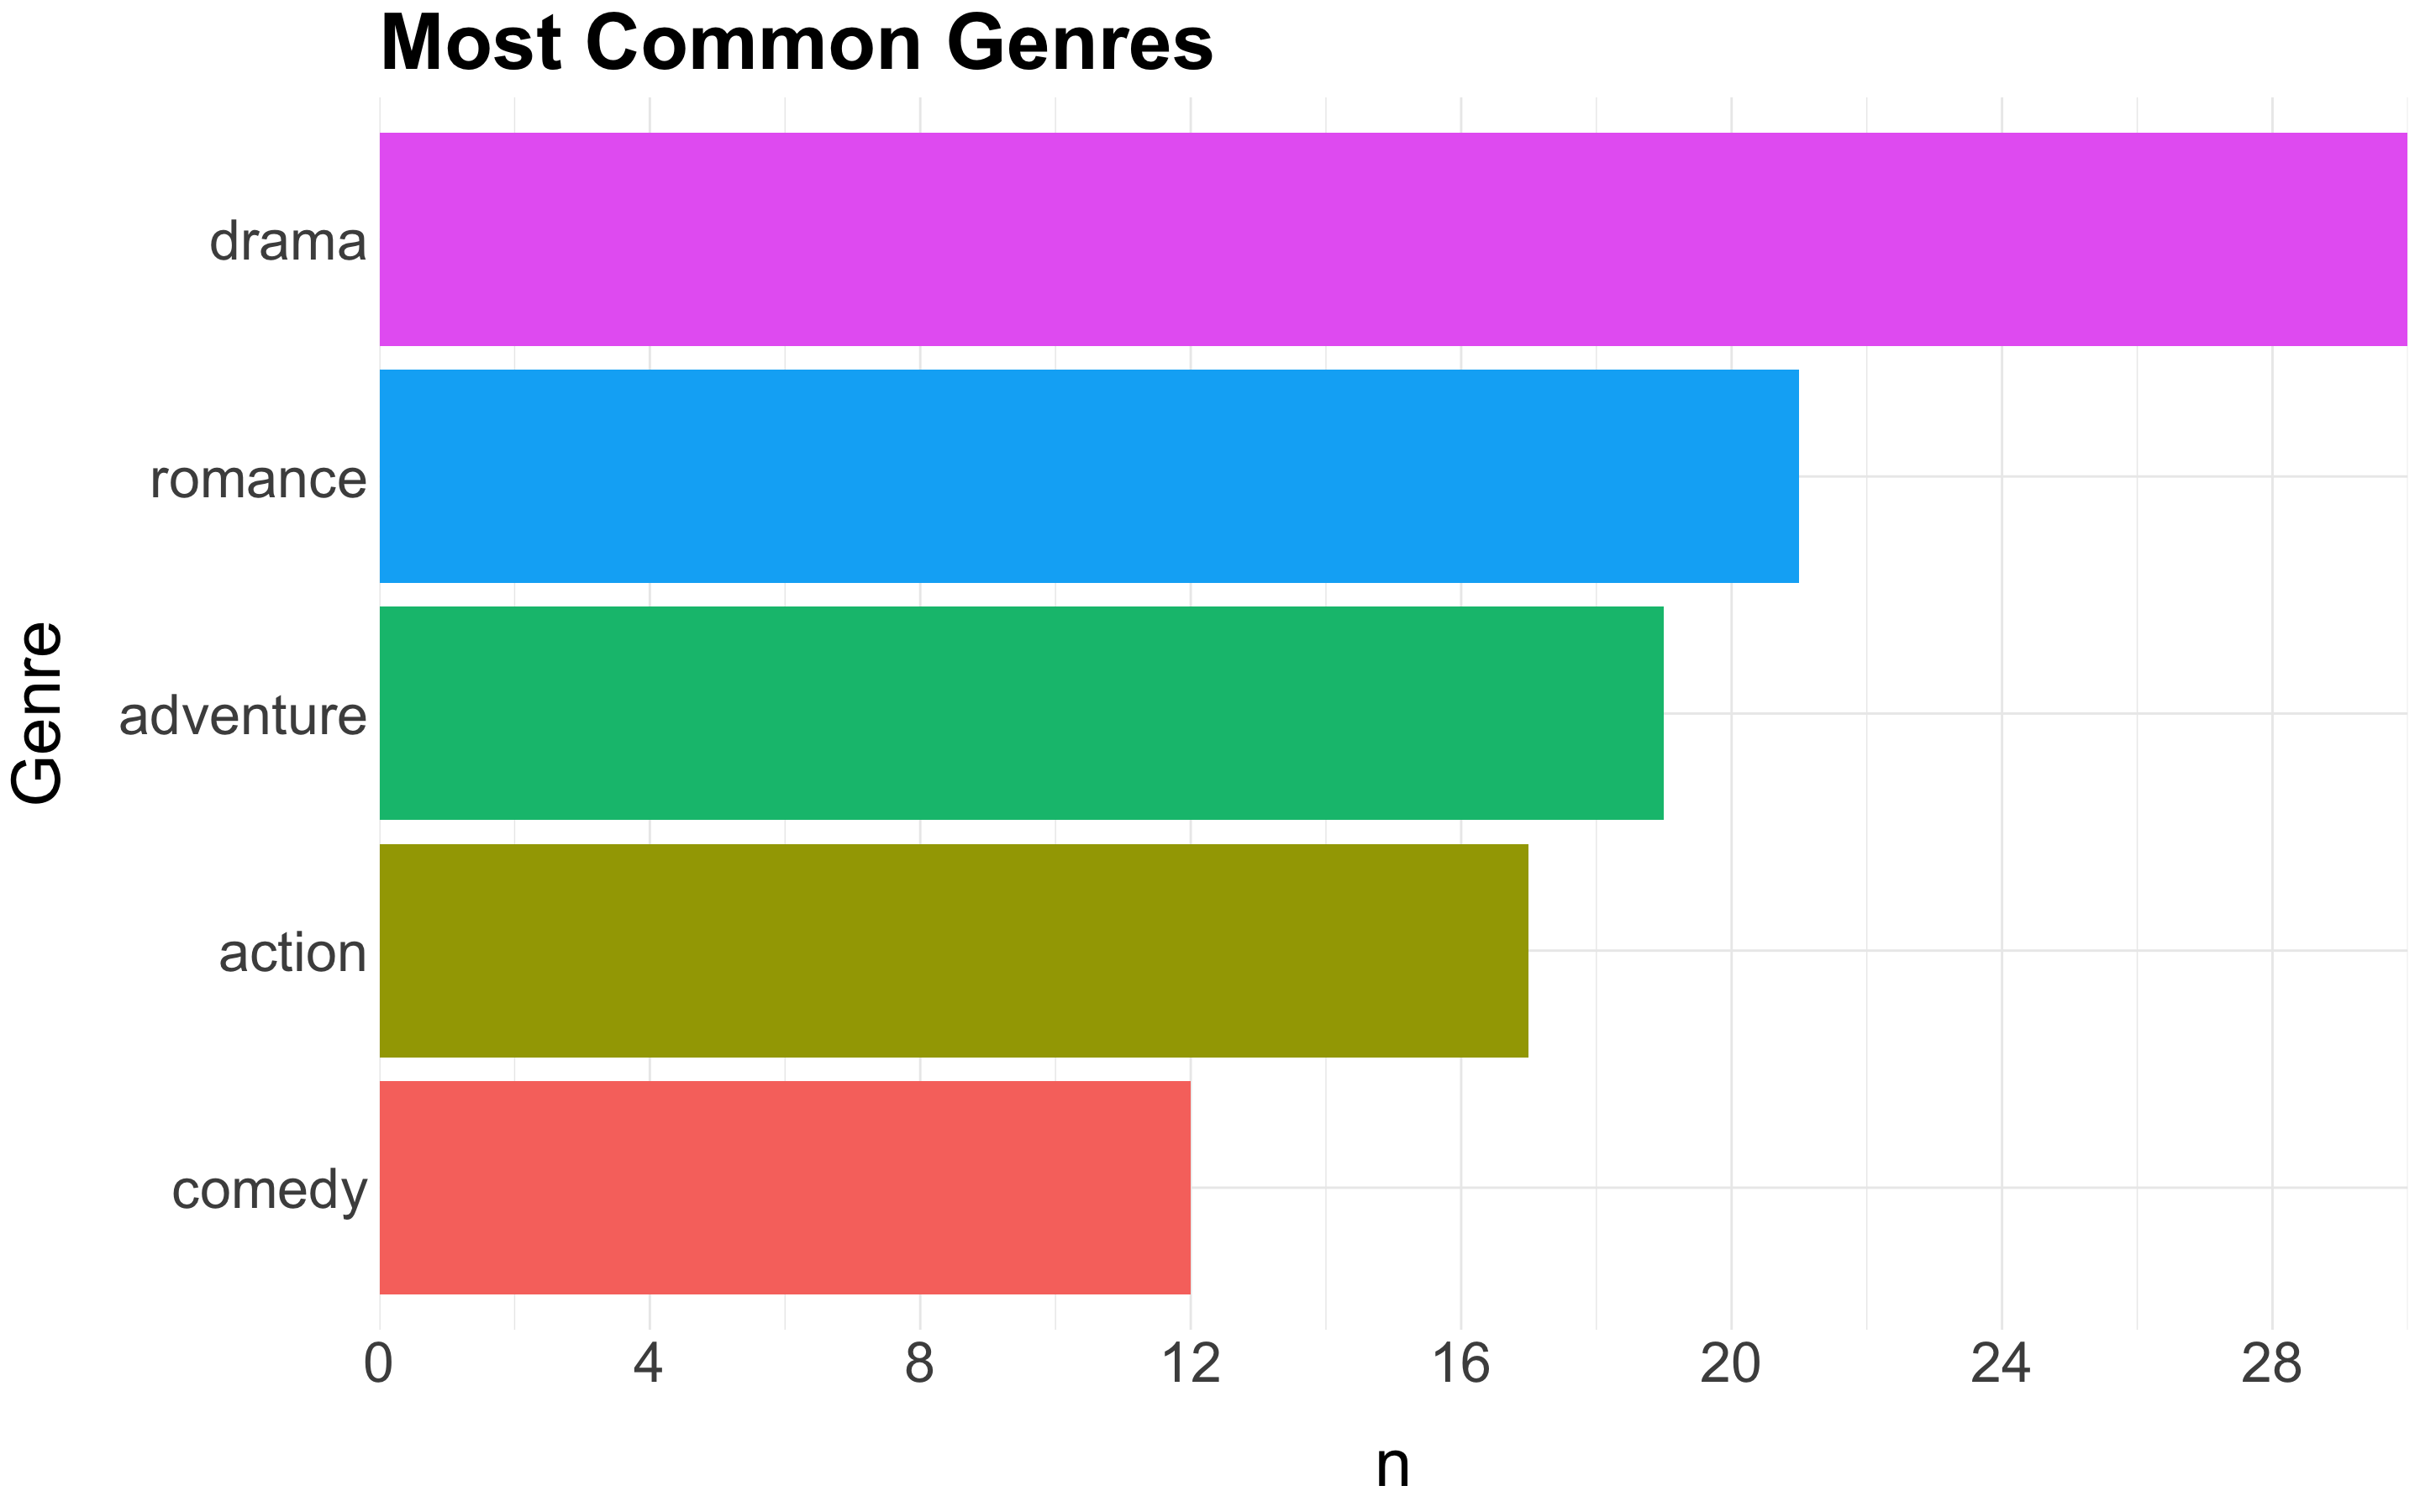
\includegraphics[width=8cm]{_assets/_assets_knn/forrest_gump_common_genres.png}
\hspace{1cm}
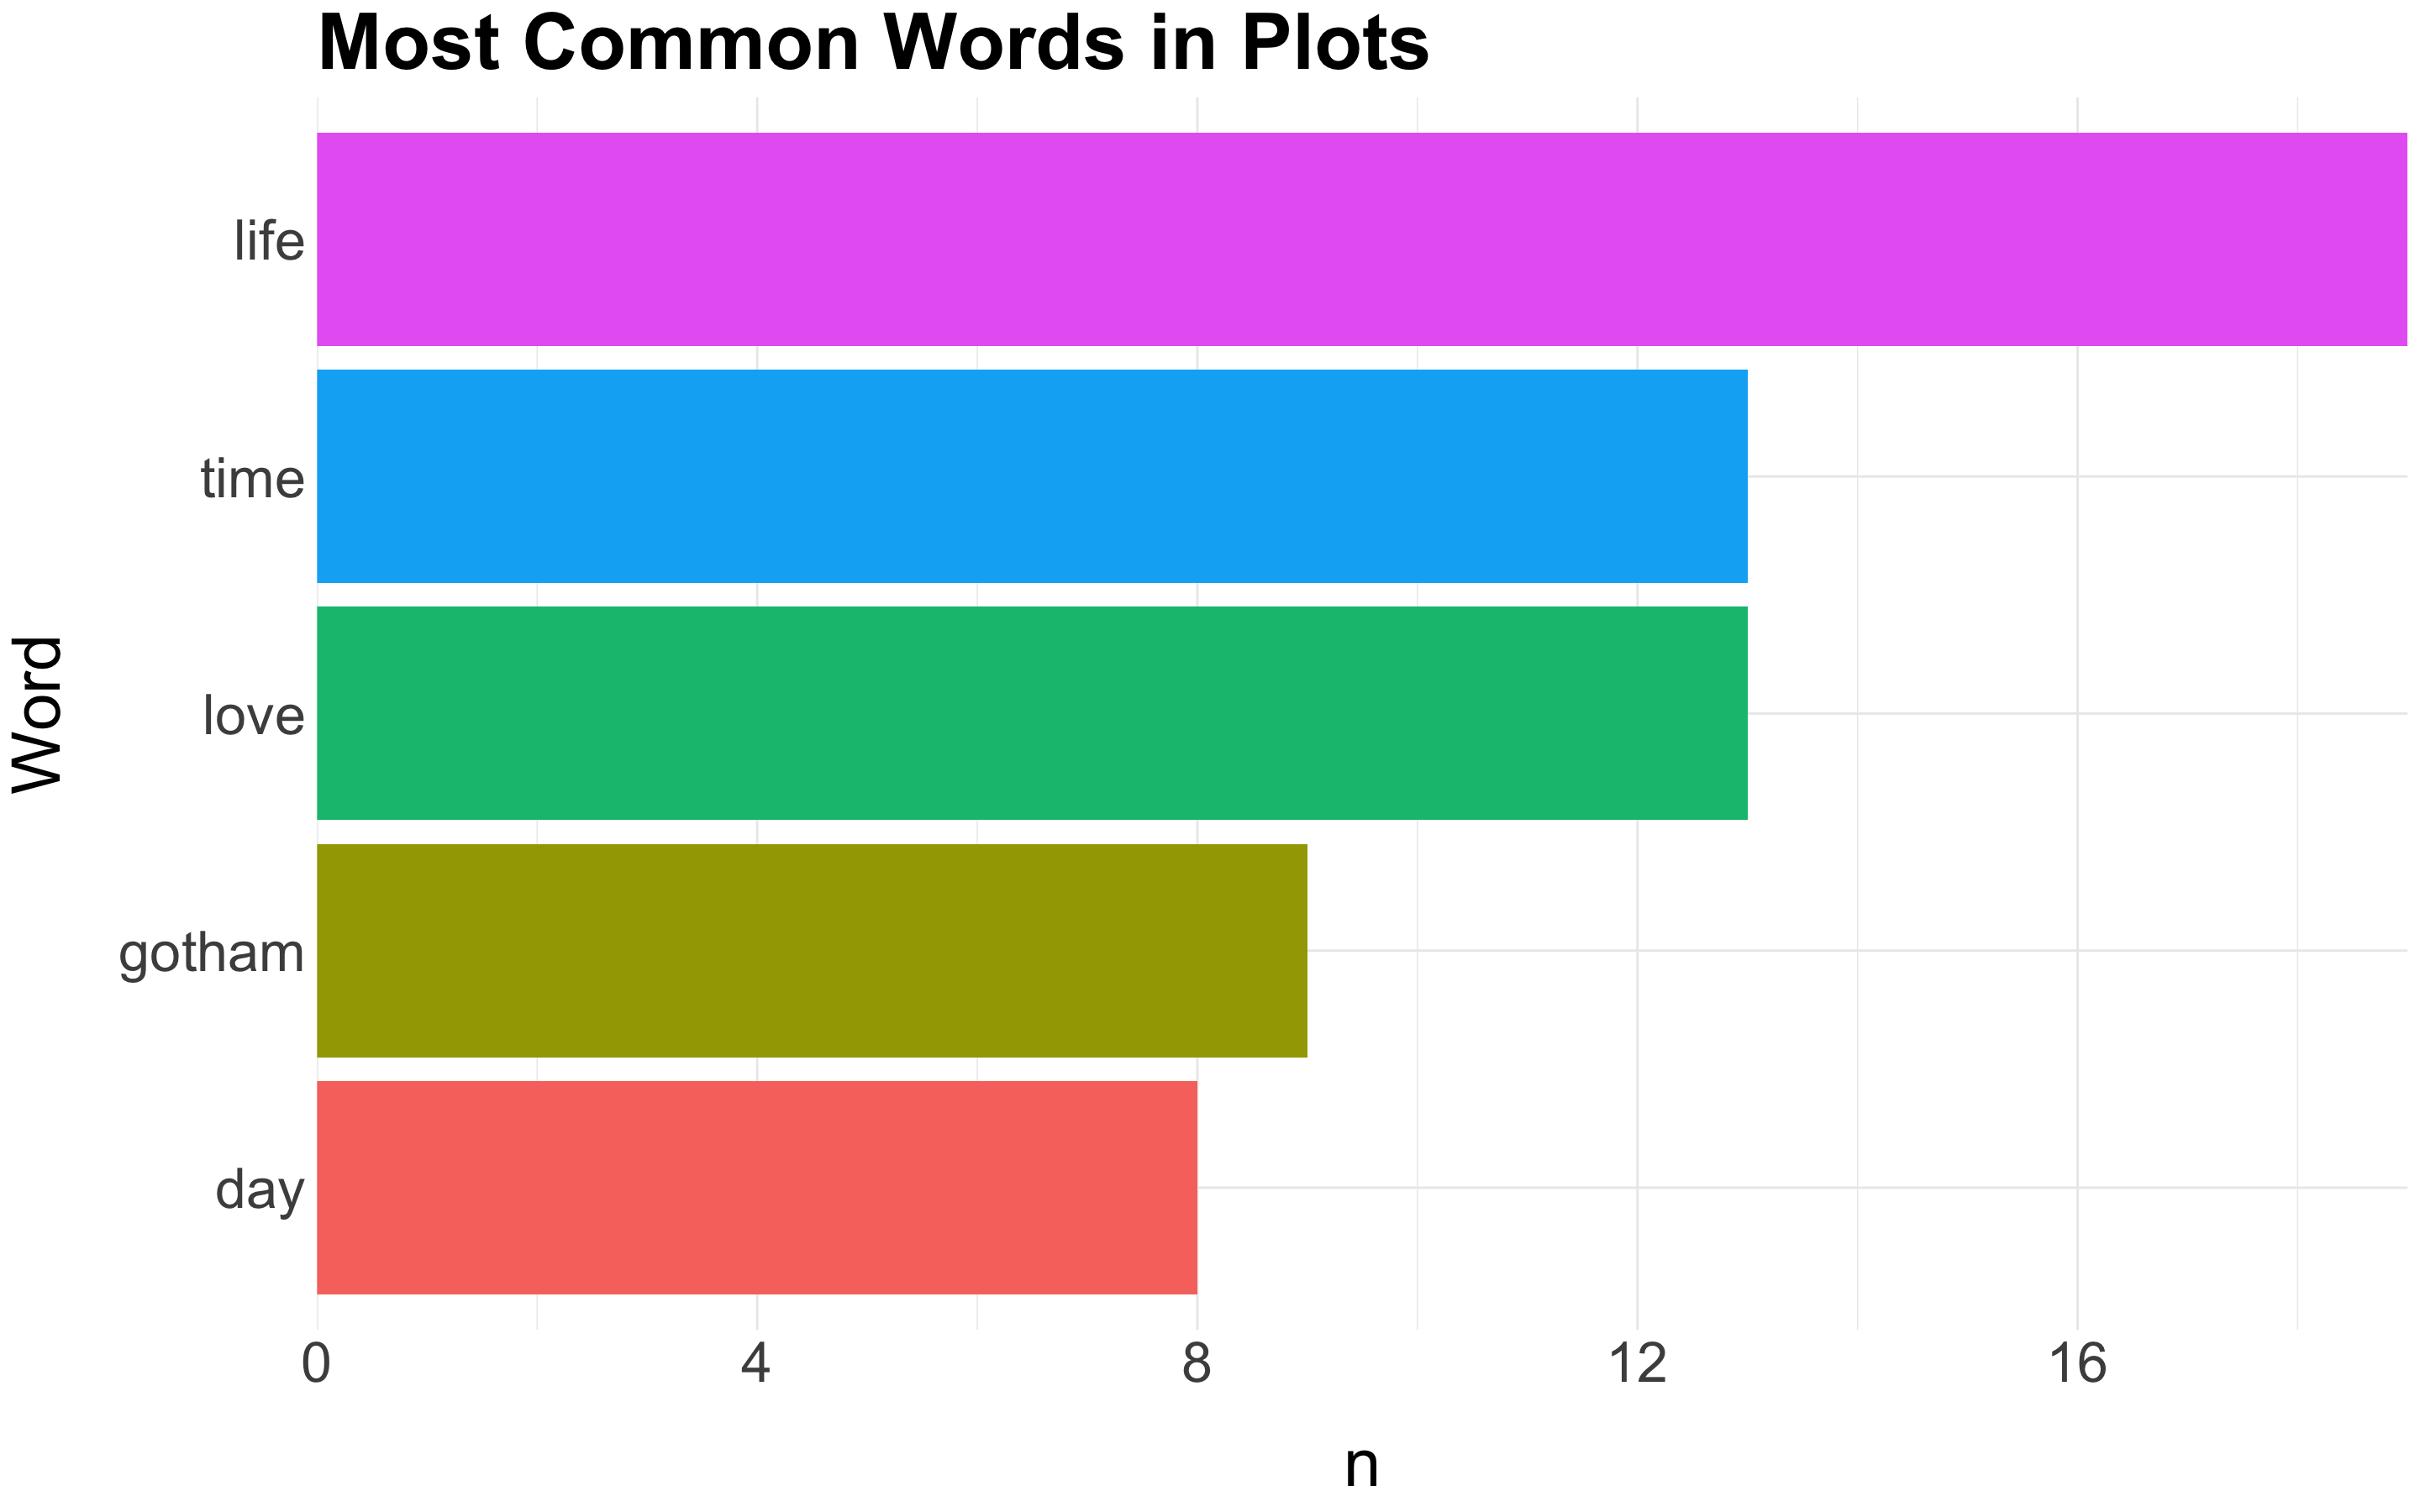
\includegraphics[width=8cm]{_assets/_assets_knn/forrest_gump_common_words.png}
% latex table generated in R 4.2.0 by xtable 1.8-4 package
% Sat Jun  4 12:48:24 2022
\begin{table}[H]
\centering
\begin{tabular}{llr}
  \hline
Full Title & Gross USA \$ & Oscar Won \\ 
  \hline
Forrest Gump (1994) & 330,455,270 &   1 \\ 
  Cast Away (2000) & 233,632,142 &   0 \\ 
  The Great Gatsby (2013) & 144,857,996 &   1 \\ 
  Tootsie (1982) & 177,200,000 &   1 \\ 
  A Beautiful Mind (2001) & 170,742,341 &   1 \\ 
  Independence Day (1996) & 306,169,268 &   1 \\ 
  Mrs. Doubtfire (1993) & 219,195,243 &   1 \\ 
  Cinderella Man (2005) & 61,649,911 &   0 \\ 
  Interstellar (2014) & 188,020,017 &   1 \\ 
  The Matrix (1999) & 172,076,928 &   1 \\ 
   \hline
\end{tabular}
\caption{The Nearest Movies to Forrest Gump (1994)} 
\end{table}


\end{center}

\section{Conclusions, Limitations, Shortcomings}
Overall, we are satisfied with the results of both our gross-profit model as well as our two Oscar-nomination prediction models. In the case of gross profit, our model achieved RMSE and R-squared values that a hypothetical producer would surely find valuable, and we also identified the most important variables to optimize in order to achieve the highest expected gross profit possible. In the case of maximizing Oscar-nomination odds, both the random forest and logistic regression models showed high accuracy and precision, with each offering insights into which variables are most important in earning an Oscar nomination. We believe these insights would prove to be highly valuable to any producer whose primary goal is to produce an Oscar-nominated film.

In addition to our predictive analyses we also achieved our goal of providing a recommendation system to producers to help them generate ideas for a movie they want to create based on films that have been made in the past. We envision producers being able to use any combination of the models and recommendations we generated to achieve their ultimate goals in creating a new film, knowing that these goals will vary between different producers. 

In terms of model limitations, the movies in the data set were still generally well known, so collecting more relatively unknown movies may provide additional insights. Additionally, the overall percent chance of any movie in our dataset receiving an Oscar nomination is less than 25\%, which may have been the reason for lower recall values in both our binary classifiers. Lastly, many variables we created based on frequency in the dataset are not completely accurate representations of how popular the stars, writers, or directors actually are or how large the production companies actually are, but we felt they worked as decent proxies given the correlations we saw with our response variables.


 \end{document}





